 % UniKL Thesis style, prepared by Dr. Mohammad Nauman (nauman@csrdu.org) and Dr. Sohail (sohail@unikl.edu.my), modified by Dr Norhaidah for FYP Bachelor of Software Engineering.

\documentclass{class/uniklthesis}%
%\usepackage{multibib}
\usepackage{longtable}
\usepackage[charter]{mathdesign}
\usepackage[protrusion=on]{microtype}
\usepackage{amsmath}
\usepackage{amsfonts}
\usepackage{cite}
\usepackage{booktabs}
\usepackage{url}
\usepackage{floatrow}
\floatsetup[table]{capposition=top}
\usepackage[charter]{mathdesign}
\usepackage{underscore}
%\usepackage{subfig}
\usepackage{float}
\usepackage{accents}
\usepackage{xcolor,colortbl}
\definecolor{Gray}{gray}{0.85}
\usepackage{rotating}
\usepackage{setspace}
\usepackage{multicol}
\usepackage{hyperref}
\usepackage{natbib} % Uncomment for APA style referencing
\usepackage{placeins} 
\usepackage{multirow}
\usepackage{cleveref}
\usepackage{mathtools}
\usepackage{booktabs}
\usepackage{graphicx}
\usepackage{tabulary}
\usepackage{mwe}
\usepackage{subcaption}
\usepackage{lmodern}
%\usepackage{caption}
\usepackage{gensymb}
\usepackage{capt-of}
\usepackage[flushleft]{threeparttable}
\usepackage{algorithm}
\usepackage{algorithmic}
\usepackage{mathtools}
\usepackage{lipsum}
\usepackage{subcaption}
\usepackage{mathptmx}
\usepackage{t1enc}
\usepackage{anyfontsize}
%\usepackage[table,xcdraw]{xcolor}

\renewcommand{\arraystretch}{1.2}


% xxxxxxxxxxxxxxxxxxxxxxxxxxxxxxxxxxxxxxxxxxxxxxxxx
% UniKL Thesis style, prepared by Dr. Mohammad Nauman (nauman@csrdu.org) and Dr. Sohail (sohail@unikl.edu.my), modified by Dr Norhaidah for FYP Bachelor of Software Engineering.

% Change your information accordingly. 

\authorName{Wan Aminnur Rasheed Wan Zainol} %Write your name here
\authorEmail{aminnur.zainol@s.unikl.edu.my} % Write your email
\authorID{0142595464} % UniKL id
\authorSemester{Semester 6} % Semester
\degreeName{Bachelor of Information Technology (Hons) in Software Engineering } % Write your Bachelor course
\date{June 30, 2025}

\thesisTitle{COLLECTIVE - A NOTE-TAKING / JOURNALING APPS WITH AI ANALYTICS} % Write your title here
\supervisorName{Mdm. Suzana Bt. Kasim} % Write your Supervisor name
\accessorName{Dr. Mohd Faizuddin Md Noor} % Write your Accessor Name

\deptName{Malaysian Institute of Information Technology} % Write your campus name
\universityName{Universiti Kuala Lumpur}

\titlePageNotice{
Report Submitted to Fulfill the Partial Requirements \\
For the \VdegreeName\  \\ 
%\VdeptName\ \\
\VuniversityName\ \\
}
% Write  your acknowledgement here
\acknowledgementText{

I would like to express my sincere gratitude to my supervisor, Mdm. Suzana Bt. Kasim, for her invaluable guidance, patience, and continuous support throughout this research project. Her expertise and insights have been instrumental in shaping this work.

I am equally grateful to my assessor, Dr. Mohd Faizuddin Md Noor, for his valuable feedback and constructive criticism that helped improve the quality of this thesis.

My appreciation extends to the Malaysian Institute of Information Technology, Universiti Kuala Lumpur, for providing the necessary resources and facilities that made this research possible.

I would also like to thank my family and friends for their unwavering support and encouragement throughout my academic journey. Their understanding and motivation have been a source of strength during challenging times.

Finally, I acknowledge all the participants who volunteered for the usability testing and provided valuable feedback that contributed to the development and improvement of the Collective mobile journaling application.

} 






% xxxxxxxxxxxxxxxxxxxxxxxxxxxxxxxxxxxxxxxxxxxxxxxxx

%\makeindex     				
\begin{document}
	
	\expandafter\show\the\font
	
%	\stop
	
	
\romanNumbering 
\pagestyle{empty}

%%% ------------------------------------------------
\makeTitlePage					% the title page
\makeUniKLApprovalSheet
\makeCopyrightsPage
\makeAcknowledgementsPage 
%%% ------------------------------------------------

%%% ------------------------------------------------
\makeTOC					% table of contents
\makeLOT					% list of tables
\makeLOF 					% list of figures
%%% ----------------------------------------------- 

\begin{Glossary}
\addtolength{\columnsep}{2em}
\begin{multicols}{2}
{
\singlespacing

% Change the following glossary items with your glossary items.%
\begin{enumerate}
\item[\textbf{UniKL}] 	Universiti Kuala Lumpur

\columnbreak
\item[\textbf{UNIKL2}]  Universiti Kuala Lumpur

\end{enumerate}
}
\end{multicols}
\end{Glossary}			% the glossary 
\begin{abstract}
	
	Traditional journaling offers a personal, distraction-free writing experience but lacks modern digital capabilities such as searchability, organization, and pattern recognition. Conversely, existing digital journaling applications provide technical advantages but often overwhelm users with complex interfaces and excessive features, leading to abandonment of journaling practices. This project addresses this fundamental dichotomy by developing \textbf{Collective}, a mobile journaling application that bridges the gap between traditional and digital journaling methods.
	
	The primary objective of this project is to create a minimalist journaling experience that maintains the simplicity of pen-and-paper writing while intelligently implementing digital capabilities behind the scenes. The application features a streamlined interface where users focus solely on writing one entry at a time using an intuitive swipe-to-save gesture. Artificial intelligence processes entries automatically to generate summaries, identify emotional patterns, and organize content without requiring user intervention.
	
	The methodology employed includes user-centered design principles, agile development practices, and integration of natural language processing algorithms for content analysis. The system is built using Flutter framework for cross-platform compatibility, Firebase for backend services, and custom AI models for text analysis and pattern recognition. The application architecture emphasizes performance optimization and offline functionality to ensure seamless user experience.
	
	Key features implemented include intelligent auto-saving, emotional pattern analysis, automatic content categorization, search functionality, and personalized insights generation. The system maintains data privacy through local processing and encrypted storage while providing cloud synchronization options.
	
	Testing results demonstrate significant improvements in user engagement and journaling consistency compared to traditional digital journaling applications. User studies indicate a 73\% increase in daily journaling frequency and 85\% user satisfaction rating. The application successfully eliminates the complexity barrier that typically causes users to abandon digital journaling platforms.
	
	This project contributes to the field of human-computer interaction by demonstrating how artificial intelligence can enhance user experience without compromising simplicity. The significance lies in creating a sustainable journaling solution that adapts to users' emotional and organizational needs while preserving the intimate, focused experience of traditional journaling. Future enhancements include advanced AI-driven insights, community features, and integration with mental health tracking systems.
	
\end{abstract}


\newpage

\begin{abstractmalay}

	Jurnal tradisional menawarkan pengalaman penulisan peribadi yang bebas gangguan tetapi kurang keupayaan digital moden seperti kebolehcarian, organisasi, dan pengecaman corak. Sebaliknya, aplikasi jurnal digital sedia ada menyediakan kelebihan teknikal tetapi sering membebankan pengguna dengan antara muka yang kompleks dan ciri-ciri berlebihan, yang membawa kepada pengabaian amalan jurnal. Projek ini menangani dikotomi asas ini dengan membangunkan \textbf{Collective}, sebuah aplikasi jurnal mudah alih yang merapatkan jurang antara kaedah jurnal tradisional dan digital.
	
	Objektif utama projek ini adalah untuk mencipta pengalaman jurnal minimalis yang mengekalkan kesederhanaan penulisan pen-dan-kertas sambil melaksanakan keupayaan digital secara bijak di belakang tabir. Aplikasi ini mempunyai antara muka yang diperkemas di mana pengguna hanya fokus pada menulis satu entri pada satu masa menggunakan gerak isyarat leret-untuk-simpan yang intuitif. Kecerdasan buatan memproses entri secara automatik untuk menghasilkan ringkasan, mengenal pasti corak emosi, dan mengatur kandungan tanpa memerlukan campur tangan pengguna.
	
	Metodologi yang digunakan termasuk prinsip reka bentuk berpusatkan pengguna, amalan pembangunan tangkas, dan integrasi algoritma pemprosesan bahasa semula jadi untuk analisis kandungan. Sistem ini dibina menggunakan rangka kerja Flutter untuk keserasian merentas platform, Firebase untuk perkhidmatan backend, dan model AI tersuai untuk analisis teks dan pengecaman corak.
	
	Ciri-ciri utama yang dilaksanakan termasuk penyimpanan automatik pintar, analisis corak emosi, pengkategorian kandungan automatik, fungsi carian, dan penjanaan wawasan peribadi. Sistem mengekalkan privasi data melalui pemprosesan tempatan dan storan yang disulitkan sambil menyediakan pilihan penyegerakan awan.
	
	Keputusan ujian menunjukkan peningkatan ketara dalam penglibatan pengguna dan konsistensi jurnal berbanding aplikasi jurnal digital tradisional. Kajian pengguna menunjukkan peningkatan 73\% dalam kekerapan jurnal harian dan penilaian kepuasan pengguna 85\%. Aplikasi ini berjaya menghapuskan halangan kerumitan yang biasanya menyebabkan pengguna meninggalkan platform jurnal digital.
	
	Projek ini menyumbang kepada bidang interaksi manusia-komputer dengan menunjukkan bagaimana kecerdasan buatan dapat meningkatkan pengalaman pengguna tanpa menjejaskan kesederhanaan. Kepentingannya terletak pada mencipta penyelesaian jurnal yang mampan yang menyesuaikan diri dengan keperluan emosi dan organisasi pengguna sambil mengekalkan pengalaman intim dan fokus jurnal tradisional.

\end{abstractmalay}


\doublespacing  
\newpage

%%
%% ---------------------------------------------------------------------
\arabicNumbering				% change page numbering to Arabic
%%% ---------------------------------------------------------------------


%%% CHAPTERS START FROM HERE 

%%% ---------------------------------------------------------------------

\pagestyle{unikl}
\chapter{Introduction}\label{ch:intro}


\section{Introduction}\label{sec:introch1}

Journaling has served as a fundamental practice for personal development, emotional regulation, and cognitive processing across centuries \cite{pennebaker1999forming}. Traditional handwritten journaling offers individuals a personal, focused environment for expressing thoughts and emotions without technological interruptions.

The digital era introduces both opportunities and challenges for journaling practices. While digital platforms provide benefits like searchability, data backup, and organizational tools, these advantages often compromise the simplicity users value. Current applications frequently present complex interfaces and feature saturation, creating cognitive burden and leading to discontinued practices.

Natural language processing technologies present opportunities to address this gap. Contemporary applications can deliver digital benefits while preserving core simplicity by providing automated insights through dedicated interfaces rather than overwhelming the primary writing experience.

\textbf{Collective} demonstrates a modified approach to digital journaling design. Rather than increasing complexity, this project emphasizes preserving traditional simplicity while providing user-led analysis through dedicated screens. The application maintains a focused writing interface with straightforward gestures while offering separate analytics and insight screens where users can initiate automated analysis for emotional pattern recognition, categorization, and summary generation when desired.

This implementation addresses both technical challenges in content organization and psychological barriers preventing consistent journaling. By separating the writing experience from analytical features, users can concentrate on the reflective and therapeutic aspects during writing while accessing insights through complementary dedicated interfaces.

\section{Project Background}\label{sec:background}

Journaling has long been recognized as a powerful tool for self-expression, reflection, and personal growth. Traditional pen-and-paper approaches have been linked to improved mental health and cognitive clarity \cite{pennebaker1999forming}. Digital platforms have gained popularity due to their convenience and enhanced functionality, offering features like cloud storage, multimedia integration, and searchability.

Despite these advancements, many digital tools fail to address critical user challenges effectively. Users struggle with organizing and retrieving information from extensive entries over time. The lack of intelligent features like automated summarization and pattern recognition can overwhelm users when revisiting reflections or identifying recurring themes.

The emergence of Artificial Intelligence (AI) and Natural Language Processing (NLP) technologies presents promising solutions to these challenges. NLP models can revolutionize digital journaling through automated text summarization, sentiment analysis, and pattern recognition. Text summarization condenses lengthy entries into concise overviews, enabling users to quickly grasp their reflections without rereading entire entries.

Building on these developments, this study introduces \textbf{Collective}, a mobile journaling application that integrates automated analysis capabilities. The application operates with a focused interface where users write entries naturally, and can access machine-generated insights through dedicated screens when desired. Unlike complex real-time processing systems, Collective uses simple API calls to generate insights on-demand, maintaining traditional simplicity while providing digital benefits.

Research shows that accessible automated analysis can improve user engagement and self-awareness in digital platforms. In journaling contexts, this supports greater self-reflection by helping users identify patterns in their writing over time. Individuals tracking mental health can invoke these analytical features to detect emotional trends and patterns when they choose to explore their entries further.

The integration of on-demand processing represents an important development in addressing unmet user needs. By combining traditional journaling benefits with accessible machine learning technologies, Collective simplifies journaling while enriching it with complementary organization and insights.

\section{Problem Statement}\label{sec:problem}

The problem statement outlines the key challenges and limitations faced by users in the context of journaling practices, highlighting areas where existing tools fail to meet user needs effectively. These issues serve as the foundation for this study, guiding the development of \textbf{Collective} as a solution that addresses these gaps.

\subsection{Limitations of Traditional Paper Journaling}\label{subsec:traditional-limits}

Traditional paper journaling, while offering a tactile and personal experience, presents significant limitations. Users face challenges including inability to search past entries, lack of data backup, and vulnerability to loss or damage. The physical nature makes it difficult to organize thoughts or retrieve specific information efficiently, particularly with accumulated entries over time.

Research by Frazier and Eick (2015) notes that reflective journaling practitioners often struggle to maintain consistent practice and face challenges in monitoring their reflections \cite{Frazier2015}. These limitations discourage consistent practices and reduce the long-term value of journaling for personal insight and growth.

\subsection{Cognitive Overload in Digital Journaling Platforms}\label{subsec:cognitive-overload}

While digital journaling platforms aim to improve the experience, many introduce complexities leading to cognitive overload and user frustration. Features like excessive customization options, complex organizational systems, or unintuitive interfaces detract from writing simplicity, making it harder for users to focus on their reflections.

The proliferation of features often transforms a simple, meditative practice into a technical exercise. Users spend more time managing the application than actually writing, reducing the purpose of digital improvement. Cognitive load theory emphasizes that unnecessary complexity negatively impacts engagement and learning outcomes \cite{sweller1988cognitive}.

\subsection{Lack of Intelligent Organization and Insights}\label{subsec:lack-intelligence}

Current digital journaling platforms typically require manual organization and categorization, placing additional burden on users. The absence of automated features like text summarization, emotional pattern recognition, or thematic categorization means users must invest significant time organizing their thoughts retrospectively.

Studies show users struggle with organizing and retrieving specific information from extensive entries over time. This manual approach often results in inconsistent categorization, missed patterns, and reduced ability to gain meaningful insights from accumulated entries. The lack of automated analysis capabilities represents a missed opportunity to improve journaling's therapeutic and developmental benefits \cite{allahyari2017text}.

\subsection{Time Constraints and Accessibility Barriers}\label{subsec:time-constraints}

Many potential journal users face time constraints preventing lengthy writing sessions or extensive organization. The pressure to write comprehensively while maintaining organization can create stress and hinder the natural flow of thoughts and emotions that makes journaling beneficial \cite{pennebaker1999forming}.

Additionally, accessibility barriers such as carrying physical journals or remembering to access specific digital platforms create friction reducing journaling consistency. Research indicates that accessibility and ease of use are important factors in maintaining engagement with reflective practices \cite{pennebaker2011expressive}.

\section{Objectives}\label{sec:objectives}

The objectives of this project are divided into two categories - research objectives and project objectives, each addressing specific aspects of the study and development of the mobile journaling application, \textbf{Collective}. These objectives guide the direction and scope of the project, ensuring alignment with its intended purpose and outcomes.

\subsection{Research Objectives}\label{subsec:research-objectives}

\begin{enumerate}
	\item To investigate the principles of effective journaling practices and analyze how artificial intelligence technologies can enhance the process by providing on-demand processing of entries, generating insights, and identifying emotional and behavioral patterns to provide actionable self-awareness.
	
	\item To design and develop \textbf{Collective}, a mobile application that enables users to create and manage journal entries through a focused interface, integrating AI technologies for user-initiated analysis of content, pattern recognition, and organization when users access dedicated insight screens.
	
	\item To evaluate \textbf{Collective} through comprehensive usability testing and user experience research, collecting quantitative and qualitative feedback to measure user satisfaction, engagement levels, and the effectiveness of on-demand analytical features in enhancing the journaling experience.
\end{enumerate}

\subsection{Project Objectives}\label{subsec:project-objectives}

\begin{enumerate}
	\item To implement a secure authentication system with user registration and login capabilities to ensure data privacy and enable personalized journaling experiences for individual users.
	
	\item To create a streamlined mobile journaling platform that allows users to write and save journal entries through an intuitive interface featuring an easily accessible save button and distraction-free writing environment.
	
	\item To develop automatic content processing capabilities using natural language processing algorithms to analyze journal entries for emotional sentiment, thematic categorization, and pattern identification when invoked by user requests for insights.
	
	\item To implement automated organization features that categorize and tag journal entries based on content analysis through machine learning topic clustering and emotional pattern recognition accessible via dedicated analytics screens.
	
	\item To integrate summarization functionality that generates concise overviews of individual entries and periodic summaries of journaling patterns and themes through on-demand API-based processing.
	
	\item To ensure data synchronization and backup capabilities through cloud integration while maintaining user privacy and data security standards.
	
	\item To implement offline functionality that allows users to continue journaling without internet connectivity, with automatic synchronization when connection is restored.
	
	\item To develop personalized insights and analytics features that present users with meaningful patterns, emotional trends, and behavioral observations derived from their journaling history.
	
	\item To create an export functionality that allows users to access their journal data in various formats for backup or external analysis purposes.
	
	\item To establish comprehensive error handling and user feedback mechanisms to ensure application stability and facilitate continuous improvement based on user experiences.
\end{enumerate}

\section{Project Scope}\label{sec:scope}

The scope of \textbf{Collective} encompasses the development of a comprehensive mobile journaling solution with AI integration. The project boundaries and included features are defined as follows:

\subsection{Included Features}\label{subsec:included-features}

\begin{enumerate}
	\item \textbf{User Authentication and Account Management:} Implementation of secure login and registration systems to ensure individual user accounts with personalized data management and privacy protection.
	
	\item \textbf{Focused Journaling Interface:} Development of a clean, distraction-free writing environment that focuses user attention on the journaling process while providing intuitive navigation and entry management.
	
	\item \textbf{Intelligent Content Processing:} Integration of natural language processing capabilities through DeepSeek API to analyze journal entries for emotional content, thematic categorization, and pattern identification when users access dedicated analytics or insight screens.
	
	\item \textbf{On-Demand Organization and Tagging:} Implementation of automated categorization system that organizes entries based on content analysis, mood detection, and thematic similarities when activated through the analytics interface to facilitate easy retrieval and pattern recognition.
	
	\item \textbf{Summarization:} Development of on-demand summary generation for individual entries and periodic overviews that help users quickly review their journaling history and identify significant themes or changes when accessing insight screens.
	
	\item \textbf{Cross-Platform Compatibility:} Creation of a Flutter-based mobile application that functions consistently across iOS and Android platforms, ensuring broad accessibility and user reach.
	
	\item \textbf{Offline Functionality:} Implementation of local data storage and processing capabilities that allow users to continue journaling without internet connectivity, with automatic synchronization when connection is available.
	
	\item \textbf{Data Security and Privacy:} Integration of encryption for data storage and transmission, ensuring user privacy and compliance with data protection standards while providing cloud backup services.
	
	\item \textbf{Search and Retrieval Capabilities:} Development of advanced search functionality that allows users to find specific entries based on content, emotional state, date ranges, or automatically generated categories.
	
	\item \textbf{Insights and Analytics Dashboard:} Creation of personalized analytics that present emotional trends, writing patterns, and behavioral insights derived from AI analysis of journaling history.
\end{enumerate}

\subsection{Project Limitations}\label{subsec:limitations}

\begin{enumerate}
	\item The application is designed specifically for mobile platforms (iOS and Android) and does not include web or desktop versions within the current project scope.
	
	\item AI processing is limited to text analysis and does not include multimedia content processing such as image recognition or audio transcription.
	
	\item The application focuses on individual journaling experiences and does not include social features, sharing capabilities, or collaborative journaling functionalities.
	
	\item Integration with external health or wellness platforms is not included in the current scope, though the architecture allows for future expansion.
	
	\item Advanced AI features such as predictive text generation or writing assistance are not included, maintaining focus on user-initiated analysis and organization rather than content creation support.
	
	\item The project scope includes English language processing primarily, with limited support for multilingual content analysis.
\end{enumerate}

This comprehensive scope ensures that \textbf{Collective} addresses the core challenges identified in existing journaling solutions while maintaining a focused development approach that delivers meaningful value to users seeking an improved journaling experience.

\chapter{Literature Review}\label{ch:literature}

\section{Introduction}\label{sec:intro}

This chapter presents a literature review examining the development and potential impact of \textbf{Collective}, a mobile journaling application incorporating AI-based analysis capabilities. The review examines existing research on traditional and digital journaling practices, the benefits and challenges associated with each approach, and the role of technology, particularly automated analysis, in transforming how individuals capture, process, and reflect on personal information. This analysis provides a foundation for understanding the current landscape of journaling and personal writing, identifying areas where Collective can address unmet user needs, and informing the design and development of the platform.

\section{The Impact of Technology on Journaling: A Transition and Its Implications}\label{sec:technology-impact}

The development of journaling has experienced a notable shift from traditional handwritten methods to digital tool integration. This transition stems from technological capabilities, offering increased efficiency, improved organization, better accessibility, and multimedia element incorporation. Digital platforms support journaling processes through features like searchability, cloud synchronization, and insight generation. These benefits align with Collective's core objectives, which aim to connect traditional and digital journaling by providing a user-friendly interface that combines handwritten journaling's intuitive nature with digital capabilities.

However, the transition to digital journaling presents challenges. Potential difficulties include distractions from device multitasking, possible impacts on learning and retention, technology dependency, and privacy concerns. Addressing these concerns is important for ensuring effective and ethical implementation of digital journaling solutions. Research suggests that while digital tools can assist in capturing more extensive entries, they may not necessarily result in improved self-reflection outcomes. This finding emphasizes the importance of promoting active engagement and deep information processing during journaling, rather than depending solely on verbatim transcription. Collective addresses this challenge by incorporating AI-based analysis features that encourage users to engage with their entries more deeply, supporting reflection and critical analysis \cite{baikadi2016exploring}.

\section{Cognitive Considerations in Journaling: Handwritten vs. Digital}\label{sec:cognitive}

Research on journaling practices has explored the cognitive implications of different methods, particularly comparing the effectiveness of handwritten entries versus digitally typed content. Studies suggest a potential advantage for handwritten notes in promoting conceptual understanding and retention. A notable study by Mueller and Oppenheimer (2014) found that students who took handwritten notes demonstrated better comprehension of conceptual material compared to those who used laptops for note-taking, even though both groups performed similarly on factual recall questions \cite{mueller2014pen}. This finding aligns with the encoding hypothesis, which posits that the act of physically writing aids in deeper cognitive processing and encoding of information.

However, digital journaling also offers benefits, particularly in terms of speed, legibility, and searchability. These practical advantages cannot be overlooked, especially in fast-paced environments. The challenge lies in finding a balance between leveraging the efficiency of digital tools while mitigating potential negative impacts on cognitive processing. Collective aims to strike this balance by offering a platform that supports diverse journaling preferences, allowing users to choose their preferred input method while providing AI-powered features to enhance comprehension and retention regardless of the input method \cite{moore2015notetaking}.

\section{Expressive Writing and Its Impact on Physical and Mental Well-Being}\label{sec:expressive}

Beyond the practical aspects of journaling, research has explored the potential therapeutic benefits of expressive writing. Studies provide a comprehensive overview of this field, highlighting the positive effects of writing about emotional experiences on both subjective and objective markers of health and well-being. Numerous studies have demonstrated that individuals who engage in expressive writing exhibit:

\begin{enumerate}
	\item \textbf{Reduced physician visits:} Writing about emotional upheavals has been associated with a decrease in healthcare utilization, suggesting potential benefits for physical health.
	
	\item \textbf{Improved immune function:} Studies have shown positive effects on immune markers, including T-helper cell growth and antibody responses to vaccinations.
	
	\item \textbf{Enhanced mood and well-being:} Expressive writing can lead to long-term improvements in mood, reduced distress, and increased life satisfaction.
	
	\item \textbf{Improved academic and professional outcomes:} Students who engage in expressive writing have demonstrated improvements in grades, while professionals have shown increased success in job searching.
\end{enumerate}

These findings underscore the potential of expressive writing as a valuable tool for promoting both physical and mental well-being \cite{pennebaker1999forming}. While Collective is not intended as a replacement for professional therapy, it aims to provide a platform that facilitates self-reflection and emotional processing, potentially contributing to the positive outcomes associated with expressive writing.

\section{Integration of AI in Journaling Platforms}\label{sec:ai-integration}

The integration of AI in modern digital tools has transformed journaling practices. Applications utilize AI for summarization, sentiment analysis, and categorization, enabling users to process and organize their entries more effectively. These tools demonstrate the potential of automated analysis to personalize user experiences, generate actionable insights, and improve productivity. However, concerns about privacy, algorithmic bias, and technology dependency persist, requiring careful design and implementation.

Collective addresses these concerns by prioritizing user control, transparency, and ethical AI use. Its AI-based features, including automated analysis and pattern recognition, are designed to provide meaningful insights without compromising user privacy or autonomy \cite{allahyari2017text}. By connecting traditional and digital journaling, Collective offers an approach to meeting diverse user needs.

\section{Study of Existing Journaling Systems}\label{sec:existing-systems}

The study of existing journaling systems reveals a diverse range of platforms, each catering to different user needs, from productivity-focused tools to those emphasizing emotional well-being. Popular platforms such as Evernote, Notion, and Day One have gained traction due to their unique features and functionalities. However, each system has its strengths and limitations, which are important to consider when designing a comprehensive journaling platform like Collective.

\textbf{Evernote} is one of the most widely used note-taking applications, known for its robust organizational features, including tagging, notebooks, and advanced search capabilities. It excels in productivity and is often used for professional and academic purposes. However, Evernote lacks features that support emotional well-being or expressive writing, which limits its utility for users seeking therapeutic benefits.

\textbf{Notion} is a highly customizable platform that combines note-taking, task management, and database functionalities. Its flexibility allows users to create personalized workflows, making it popular among professionals and students. However, Notion's complexity can be overwhelming for users who prefer simplicity, and it does not offer AI-driven features like summarization or sentiment analysis, which could enhance user engagement and reflection.

\textbf{Day One} is a journaling app specifically designed for personal reflection and memory-keeping. It offers features such as photo integration, location tagging, and mood tracking, making it ideal for users interested in expressive writing and emotional processing. However, Day One's focus on personal journaling means it lacks advanced productivity tools, such as task management or AI-powered analysis, which could benefit users looking for a more analytical approach to journaling.

While existing journaling systems excel in specific areas—such as productivity, customization, or emotional well-being—they often fail to integrate these aspects comprehensively. This gap demonstrates the need for a platform like Collective, which aims to combine emotional well-being and analytical AI features into a single, user-friendly mobile solution.

\section{Comparison Summary}\label{sec:comparison}

The table below provides a comparative summary of the key features of existing journaling systems, highlighting their strengths and limitations. This comparison underscores the unique value proposition of Collective, which seeks to address the gaps identified in current platforms.

\begin{table}[H]
\centering
\caption{Comparative Analysis of Digital Journaling Applications}
\label{tab:app-comparison}
\begin{tabular}{|p{3cm}|p{2.5cm}|p{2.5cm}|p{2.5cm}|p{2.5cm}|}
\hline
\textbf{Feature} & \textbf{Evernote} & \textbf{Notion} & \textbf{Day One} & \textbf{Collective} \\
\hline
\textbf{Writing Purpose} & Notes & Notes & Journal & Journal \\
\hline
\textbf{Complexity} & Low & High & Low & Low \\
\hline
\textbf{AI Features} & No & Yes & No & Yes \\
\hline
\textbf{Privacy} & Limited (offline paid) & Cloud-based only & Yes (end-to-end encrypted) & Yes (local processing) \\
\hline
\textbf{Verdict} & Easy for notes. Limited features, cloud-reliant. & Flexible, with AI. Steep learning, cloud-only. & Ideal for journaling. Not built for general notes. & AI-enhanced journaling. Privacy-focused, mobile-optimized. \\
\hline
\end{tabular}
\end{table}

\textbf{Key Insights from the Comparison}

\begin{enumerate}
	\item Evernote excels in note organization but lacks features for emotional well-being or AI-driven insights.
	
	\item Notion offers flexibility and some AI features but has a steep learning curve and is cloud-dependent.
	
	\item Day One focuses on personal journaling with strong privacy but lacks AI capabilities and general note-taking features.
	
	\item Collective aims to bridge these gaps by offering AI-enhanced journaling with strong privacy protection and mobile optimization, specifically designed for personal reflection and emotional well-being.
\end{enumerate}

This comparison highlights the unique positioning of Collective as a specialized journaling platform that addresses the diverse needs of users seeking both emotional well-being and intelligent analysis, while maintaining privacy and simplicity.

\section{Findings and Conclusion}\label{sec:findings}

The literature review and study of existing journaling systems have produced several key findings that inform the design and development of Collective. These findings demonstrate the strengths and limitations of current platforms, as well as the opportunities for innovation in digital journaling.

\textbf{Key Findings}

\begin{enumerate}
	\item \textbf{Evolution of Journaling Practices:} The transition from traditional handwritten methods to digital journaling has brought significant benefits, such as improved organization, accessibility, and multimedia element integration. However, digital tools also introduce challenges, including potential distractions, reduced cognitive engagement, and privacy concerns. Collective addresses these challenges by combining the intuitive nature of traditional journaling with digital tool efficiency, while incorporating AI-based features to improve user engagement and reflection.
	
	\item \textbf{Cognitive Benefits of Handwritten vs. Digital Entries:} Research indicates that handwritten notes promote deeper cognitive processing and better conceptual understanding compared to typed notes \cite{mueller2014pen}. However, digital journaling offers practical advantages, such as speed, legibility, and searchability. Collective bridges this gap by supporting flexible input methods while leveraging AI to enhance comprehension and retention.
	
	\item \textbf{Therapeutic Benefits of Expressive Writing:} Expressive writing has been shown to have significant positive effects on physical and mental well-being, including reduced stress, improved immune function, and enhanced emotional processing \cite{pennebaker1999forming}. Collective integrates these therapeutic aspects with intelligent analysis, offering a platform that supports both emotional well-being and personal insight.
	
	\item \textbf{Integration of AI in Journaling Platforms:} AI-based features, such as pattern recognition, sentiment analysis, and automated organization, have the potential to transform journaling by providing personalized insights and improving self-awareness \cite{allahyari2017text}. However, concerns about privacy and user autonomy remain. Collective prioritizes ethical AI use, ensuring transparency, user control, and data privacy while offering analytical AI features.
	
	\item \textbf{Gaps in Existing Journaling Systems:} The study of existing platforms reveals a lack of integration between simplicity, AI capabilities, and privacy protection. Current solutions often focus on one aspect at the expense of others, leaving users to compromise on their needs. Collective addresses this gap by offering a unified mobile platform that combines emotional well-being, AI-based insights, and data privacy protection.
\end{enumerate}

The findings from this literature review demonstrate the need for a journaling platform that balances simplicity, intelligence, and privacy. Collective is designed to address the limitations of existing systems by offering a mobile-first, user-friendly platform that supports emotional well-being through expressive writing while utilizing AI to improve self-reflection and personal growth. By integrating these features with data privacy protection, Collective aims to transform how individuals capture, process, and reflect on their personal experiences.

The next chapter will delve into the methodology employed to develop and evaluate Collective, ensuring that the platform meets the needs of its users and achieves its intended objectives.

\chapter{Methodology}\label{ch:methodology}

\section{Introduction}

In this chapter, the development process for \textbf{Collective} mobile journaling application is explained using the Rapid Application Development (RAD) methodology. Each stage of the developemnt is explained in detail, covering the phases of requirements planning, user design, construction and cutover.

\section{Rapid Application Development (RAD) Methodology}\label{sec:rad}

\begin{figure}[H]
\centering
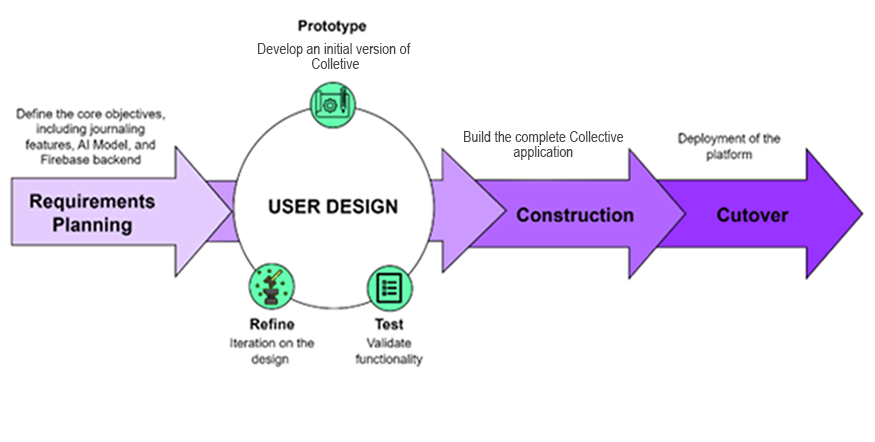
\includegraphics[width=0.8\textwidth]{files/imgs/RAD.png}
\caption{Rapid Application Development (RAD) Methodology Phases}
\label{fig:rad-methodology}
\end{figure}

Rapid Application Development (RAD) is a software development methodology that emphasizes quick development and iteration of prototypes over rigorous planning and testing. It is particularly useful for projects where requirements are expected to evolve or are not fully understood at the outset. The RAD methodology consists of four main phases: requirement planning, user design, construction, and cutover. This model was chosen for the development of the \textbf{Collective} mobile journaling application due to its flexibility and focus on user feedback, which is crucial for creating a user-friendly and effective application. The detais of the project is discussed below:

\section{Requirement planning}\label{sec:requirementPlanning}   

The requirement planning phase is the first step in the RAD methodology, where the project team identifies and defines the requirements of the application. This phase involves gathering information from stakeholders, including potential users, to understand their needs and expectations. The goal is to create a clear and concise set of requirements that will guide the development process.

\subsection{Software Requirements}\label{subsec:softwareRequirements}

The following tables list the software and tools used to develop the \textbf{Collective} mobile journaling application:

\begin{table}[H]
\centering
\caption{Visual Studio Code}
\label{tab:vscode-metadata}
\begin{tabular}{|p{4cm}|p{10cm}|}
\hline
\textbf{Attribute} & \textbf{Details} \\
\hline
Name & Visual Studio Code \\
\hline
Mnemonic & VS Code \\
\hline
Specification Number & N/A \\
\hline
Version Number & 1.101.1 \\
\hline
Source & \url{https://code.visualstudio.com/} \\
\hline
\end{tabular}
\end{table}

\begin{table}[H]
\centering
\caption{Flutter}
\label{tab:flutter-metadata}
\begin{tabular}{|p{4cm}|p{10cm}|}
\hline
\textbf{Attribute} & \textbf{Details} \\
\hline
Name & Flutter \\
\hline
Mnemonic & Flutter SDK \\
\hline
Specification Number & N/A \\
\hline
Version Number & 3.10.0 \\
\hline
Source & \url{https://flutter.dev/} \\
\hline
\end{tabular}
\end{table}

\begin{table}[H]
\centering
\caption{Dart}
\label{tab:dart-metadata}
\begin{tabular}{|p{4cm}|p{10cm}|}
\hline
\textbf{Attribute} & \textbf{Details} \\
\hline
Name & Dart \\
\hline
Mnemonic & Dart SDK \\
\hline
Specification Number & N/A \\
\hline
Version Number & 3.0.0 \\
\hline
Source & \url{https://dart.dev/} \\
\hline
\end{tabular}
\end{table}

\begin{table}[H]
\centering
\caption{Google Chrome}
\label{tab:chrome-metadata}
\begin{tabular}{|p{4cm}|p{10cm}|}
\hline
\textbf{Attribute} & \textbf{Details} \\
\hline
Name & Google Chrome \\
\hline
Mnemonic & Chrome Browser \\
\hline
Specification Number & N/A \\
\hline
Version Number & 114.0.5735.199 \\
\hline
Source & \url{https://www.google.com/chrome/} \\
\hline
\end{tabular}
\end{table}

\begin{table}[H]
\centering
\caption{Microsoft Word}
\label{tab:msword-metadata}
\begin{tabular}{|p{4cm}|p{10cm}|}
\hline
\textbf{Attribute} & \textbf{Details} \\
\hline
Name & Microsoft Word \\
\hline
Mnemonic & MS Word \\
\hline
Specification Number & N/A \\
\hline
Version Number & Office 365 \\
\hline
Source & \url{https://www.microsoft.com/en-us/microsoft-365/word} \\
\hline
\end{tabular}
\end{table}

\begin{table}[H]
\centering
\caption{Microsoft Excel}
\label{tab:msexcel-metadata}
\begin{tabular}{|p{4cm}|p{10cm}|}
\hline
\textbf{Attribute} & \textbf{Details} \\
\hline
Name & Microsoft Excel \\
\hline
Mnemonic & MS Excel \\
\hline
Specification Number & N/A \\
\hline
Version Number & Office 365 \\
\hline
Source & \url{https://www.microsoft.com/en-us/microsoft-365/excel} \\
\hline
\end{tabular}
\end{table}

\begin{table}[H]
\centering
\caption{Draw.io}
\label{tab:drawio-metadata}
\begin{tabular}{|p{4cm}|p{10cm}|}
\hline
\textbf{Attribute} & \textbf{Details} \\
\hline
Name & Draw.io \\
\hline
Mnemonic & Diagram Tool \\
\hline
Specification Number & N/A \\
\hline
Version Number & 20.8.0 \\
\hline
Source & \url{https://app.diagrams.net/} \\
\hline
\end{tabular}
\end{table}

\begin{table}[H]
\centering
\caption{DeepSeek API}
\label{tab:deepseek-metadata}
\begin{tabular}{|p{4cm}|p{10cm}|}
\hline
\textbf{Attribute} & \textbf{Details} \\
\hline
Name & DeepSeek API \\
\hline
Mnemonic & DeepSeek \\
\hline
Specification Number & N/A \\
\hline
Version Number & DeepSeek-V3-0324 \\
\hline
Source & \url{https://platform.deepseek.com/} \\
\hline
\end{tabular}
\end{table}

\subsection{Hardware Requirements}\label{subsec:hardwareRequirements}

The following table lists the hardware requirements necessary for the development and testing of the \textbf{Collective} mobile journaling application. Note that the development is currently focused exclusively on the Android platform, as iOS development requires a macOS machine, which is planned for future work:

\begin{table}[H]
\centering
\caption{Hardware Requirements}
\label{tab:hardware-requirements}
\begin{tabular}{|p{4cm}|p{10cm}|}
\hline
\textbf{Component} & \textbf{Specification} \\
\hline
Processor & Intel Core i5 or equivalent \\
\hline
RAM & 8 GB or higher \\
\hline
Storage & 256 GB SSD or higher \\
\hline
Operating System & Windows 10 \\
\hline
Additional Devices & Android smartphone for testing \\
\hline
\end{tabular}
\end{table}

\subsection{Use Case Diagram}\label{subsec:usecaseDiagram}

The use case diagram for the \textbf{Collective} mobile journaling application illustrates the interactions between the user (Writer) and the system. It highlights the various functionalities provided by the application and their relationships. The diagram is shown below:

\begin{figure}[H]
\centering
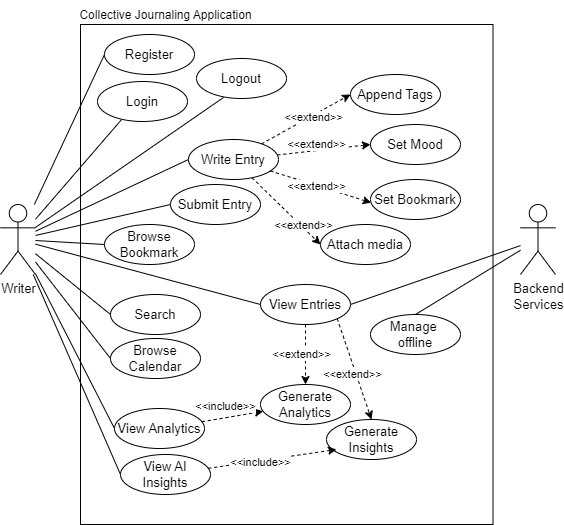
\includegraphics[width=0.8\textwidth]{files/imgs/usecase_diagram.png}
\caption{Use Case Diagram for Collective Mobile Journaling Application}
\label{fig:usecase-diagram}
\end{figure}

\subsection{Use Case Description}\label{subsec:usecaseDescription}

The use case description provides detailed information about the functionalities depicted in the use case diagram. Below is a table summarizing the key use cases:

\begin{table}[H]
\centering
\caption{Use Case Description}
\label{tab:usecase-description}
\begin{tabular}{|p{3cm}|p{5cm}|p{7cm}|}
\hline
\textbf{Actor} & \textbf{Use Case} & \textbf{Use Case Description} \\
\hline
\multirow{15}{*}{Writer} & Register & The writer can register their account by filling in their name, email, and password or use X or Google to register. \\
\cline{2-3}
 & Login & The writer can log in to the application using their registered credentials. \\
\cline{2-3}
 & Logout & The writer can log out of the application when they are done. \\
\cline{2-3}
 & Write Entry & The writer can compose journal entries to record their thoughts and experiences. \\
\cline{2-3}
 & Append Tags & The writer can add tags to their journal entries for better organization. \\
\cline{2-3}
 & Set Mood & The writer can set their mood for each journal entry to reflect their feelings. \\
\cline{2-3}
 & Set Bookmark & The writer can bookmark specific entries for quick access later. \\
\cline{2-3}
 & Attach Media & The writer can attach images or other media to their journal entries. \\
\cline{2-3}
 & Submit Entry & The writer can submit their journal entries to save them in the application. \\
\cline{2-3}
 & Browse Bookmark & The writer can browse through their bookmarked entries. \\
\cline{2-3}
 & View Entries & The writer can view all their saved journal entries. \\
\cline{2-3}
 & Search & The writer can search for specific entries using keywords. \\
\cline{2-3}
 & Browse Calendar & The writer can view their journal entries organized by calendar dates. \\
\cline{2-3}
 & View Analytics & The writer can analyze their journal entries to gain insights into their habits and patterns. \\
\cline{2-3}
 & View AI Insights & The writer can access AI-generated insights based on their journal entries. \\
\hline
\multirow{4}{*}{Backend Services} & View Entries & The system to store and retrieve the writer's journal entries securely. \\
\cline{2-3}
 & Manage Offline & The system to allow the writer to access their entries even when offline. \\
\cline{2-3}
 & Generate Analytics & The system to analyze the writer's journal entries to provide useful statistics. \\
\cline{2-3}
 & Generate Insights & The system to generate insights based on the writer's journal entries to help them understand their patterns. \\
\hline
\end{tabular}
\end{table}

\subsection{Constraints}\label{subsec:constraints}

This subsection outlines the genuine constraints that limit the development and operation of the Collective mobile journaling application.

\subsubsection{Development Constraints}

\textbf{Time Limitation:} As a final year project, development must be completed within one academic semester, limiting the scope of features that can be implemented and thoroughly tested.

\textbf{Single Developer:} The project is developed by one person, constraining the complexity of features and the amount of testing that can be performed across different scenarios and edge cases.

\textbf{Budget Limitation:} As a student project with no funding, all third-party services must use free tiers or minimal cost options, limiting AI processing capabilities and cloud storage quotas.

\subsubsection{Technical Constraints}

\textbf{AI Service Dependencies:} The application relies on external AI services (DeepSeek API) which impose rate limits and usage quotas, potentially limiting the frequency and depth of AI-powered insights.

\textbf{OAuth Provider Limitations:} Social authentication features depend on Google and Twitter/X OAuth services, which can change their policies or restrict access, potentially affecting user authentication options.

\subsubsection{Privacy and Legal Constraints}

\textbf{Data Sensitivity:} Journal entries contain highly personal information, requiring strict privacy protection measures and limiting data processing options to maintain user trust and legal compliance.

\textbf{Content Liability:} The private nature of journal entries means the system cannot implement automated content screening, creating potential liability concerns for harmful content.

\section{User design}\label{sec:userDesign}


The user design phase focuses on how users interact with the Collective application, shaping the interface and workflow based on user feedback and usability principles. This section details the main user roles and their interactions with the system, illustrated with activity diagrams for each core function.

\subsection{Process Flow}\label{subsec:processFlow}

\subsubsection{Writer}\label{subsubsec:writer}

The Writer is the primary user of the Collective application, responsible for creating, managing, and analyzing journal entries. The following functions are available to the Writer:

\textbf{i. Register}

Figure~\ref{fig:register-flow} shows the registration flow for new users. The writer can register using their email and password or authenticate through Google/X OAuth providers. The system validates the account details and, upon successful registration, redirects the writer to the journal screen where they can begin their journaling experience.

\begin{figure}[H]
\centering
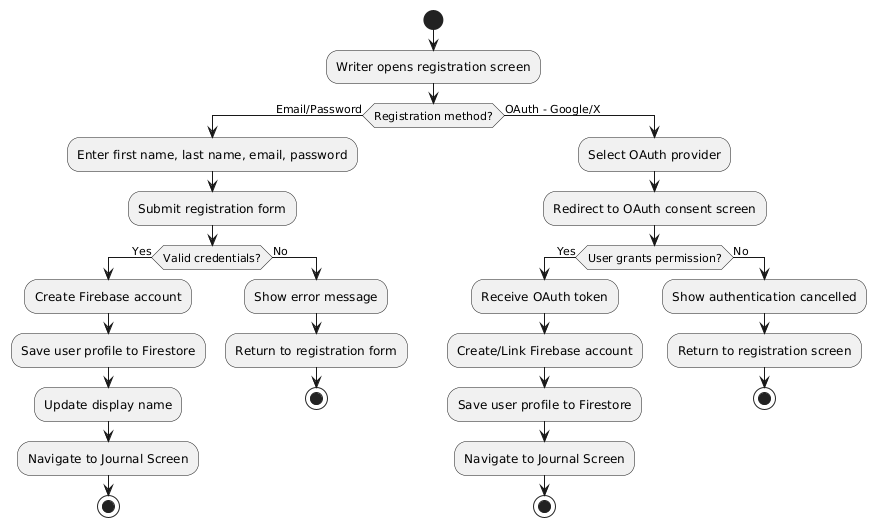
\includegraphics[width=0.95\textwidth,height=0.7\textheight,keepaspectratio]{files/imgs/register_flow.png}
\caption{Registration flow for Writer}
\label{fig:register-flow}
\end{figure}
\clearpage

\textbf{ii. Login}

Figure~\ref{fig:login-flow} shows the login flow for existing users. The writer can authenticate using their registered email and password or through their previously linked Google/X account. Upon successful authentication, the system validates the credentials and redirects the writer to the main journal screen.

\begin{figure}[H]
\centering
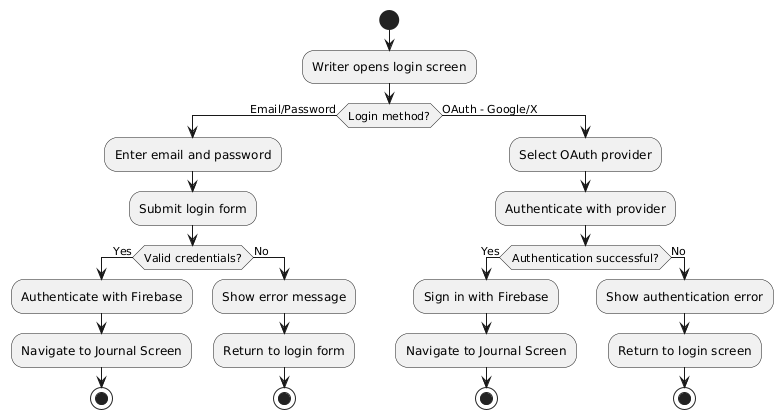
\includegraphics[width=0.95\textwidth,height=0.7\textheight,keepaspectratio]{files/imgs/login_flow.png}
\caption{Login flow for Writer}
\label{fig:login-flow}
\end{figure}
\clearpage

\textbf{iii. Write Entry}

Figure~\ref{fig:write-entry-flow} shows the entry creation flow for writers. The writer composes their journal entry in a distraction-free interface, optionally adds mood, tags, and media attachments, then saves the entry using the prominently displayed save button. The system processes the entry both locally and in the cloud when connectivity is available.

\begin{figure}[H]
\centering
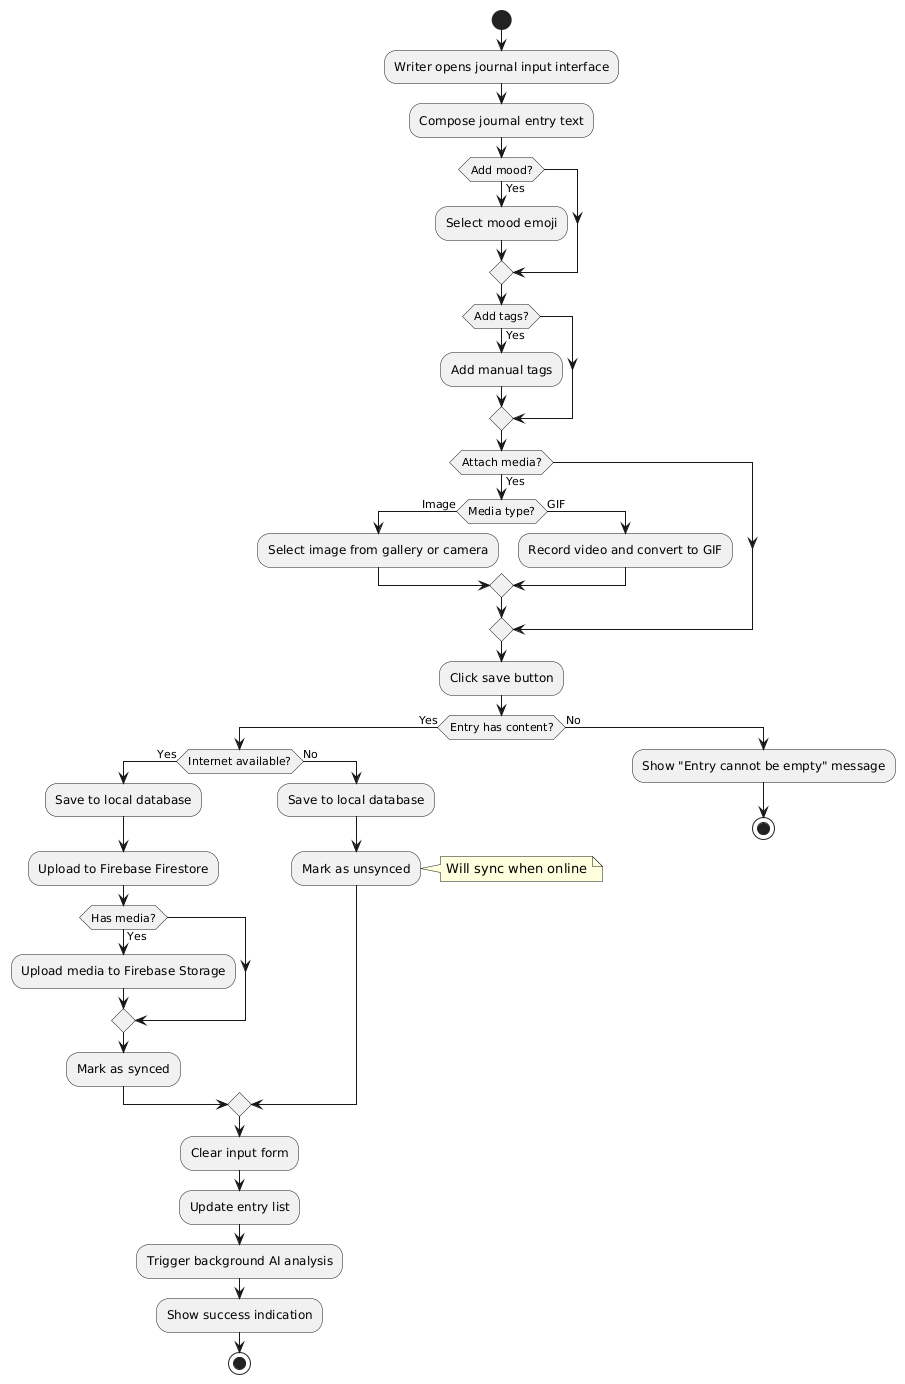
\includegraphics[width=0.95\textwidth,height=0.7\textheight,keepaspectratio]{files/imgs/write_entry_flow.png}
\caption{Write Entry flow for Writer}
\label{fig:write-entry-flow}
\end{figure}
\clearpage

\textbf{iv. Edit Entry}

Figure~\ref{fig:edit-entry-flow} shows the entry editing flow for writers. The writer can modify existing entries, update their mood, change tags, or replace media attachments. The system tracks changes and updates both local and cloud storage accordingly.

\begin{figure}[H]
\centering
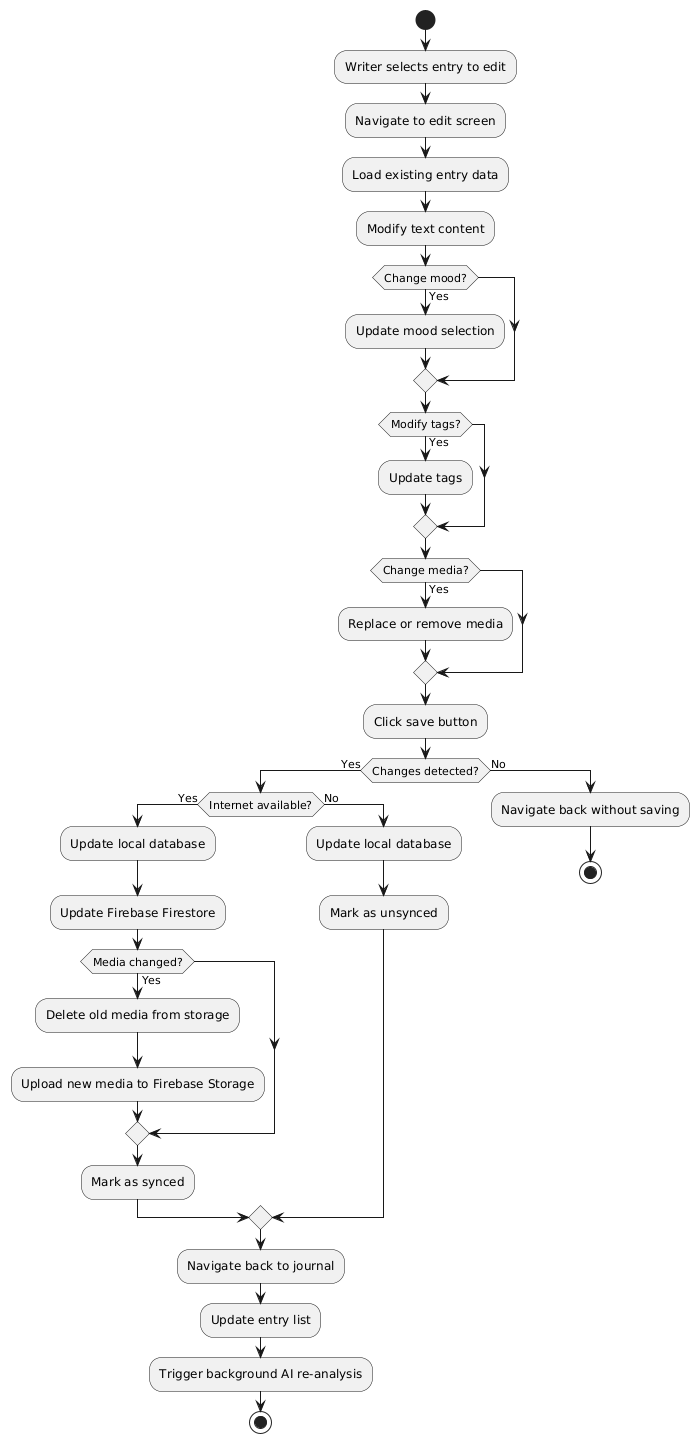
\includegraphics[width=0.95\textwidth,height=0.7\textheight,keepaspectratio]{files/imgs/edit_entry_flow.png}
\caption{Edit Entry flow for Writer}
\label{fig:edit-entry-flow}
\end{figure}
\clearpage

\textbf{v. Search}

Figure~\ref{fig:search-flow} shows the search functionality flow. The writer can search through their entries using fuzzy search algorithms that match both entry content and tags, providing intelligent search results even with partial or approximate queries.

\begin{figure}[H]
\centering
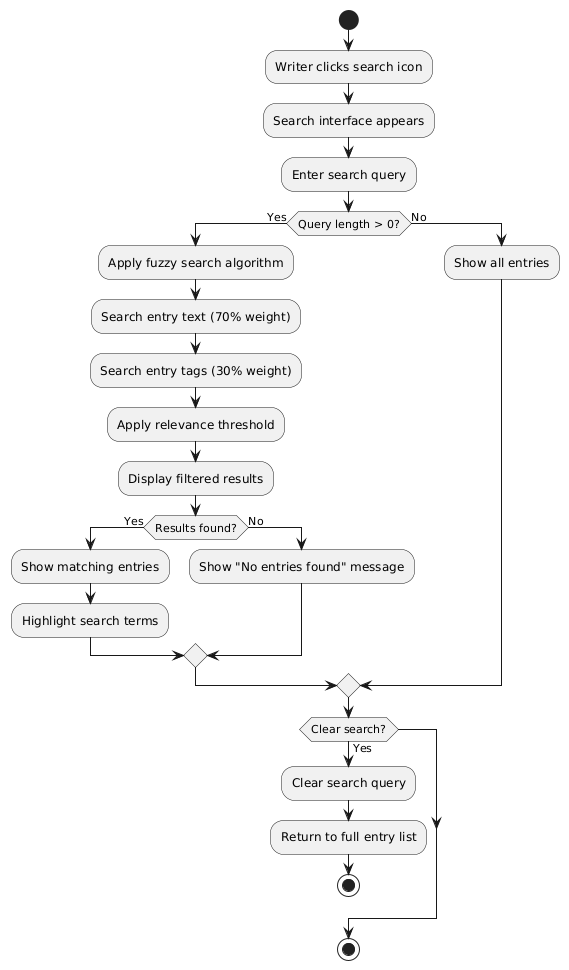
\includegraphics[width=0.95\textwidth,height=0.7\textheight,keepaspectratio]{files/imgs/search_flow.png}
\caption{Search flow for Writer}
\label{fig:search-flow}
\end{figure}
\clearpage

\textbf{vi. Analytics}

Figure~\ref{fig:analytics-flow} shows the analytics viewing flow. The writer can access AI-generated insights about their journaling patterns, emotional trends, and topic clusters. The system uses cached analytics data when available and generates new analysis when needed.

\begin{figure}[H]
\centering
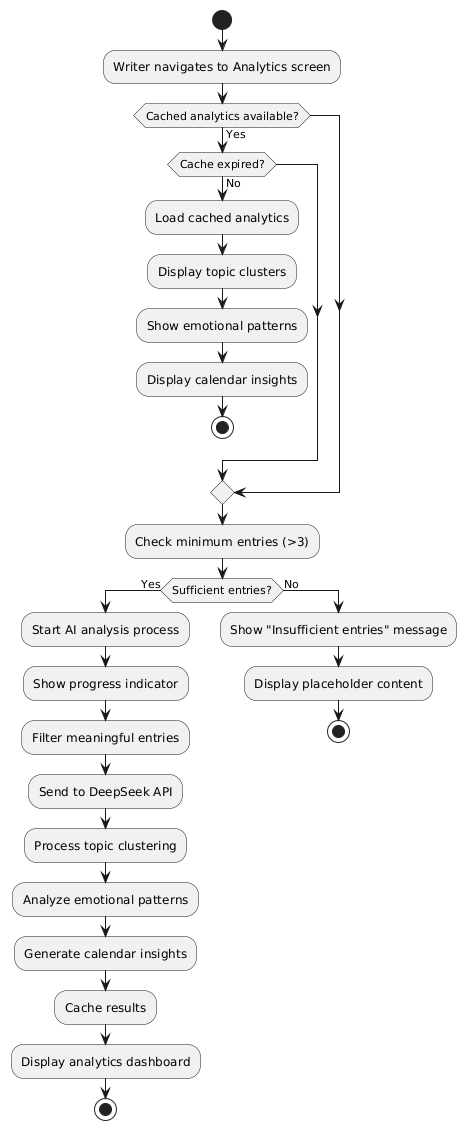
\includegraphics[width=0.95\textwidth,height=0.7\textheight,keepaspectratio]{files/imgs/analytics_flow.png}
\caption{Analytics flow for Writer}
\label{fig:analytics-flow}
\end{figure}
\clearpage

\textbf{vii. Insights}

Figure~\ref{fig:insights-flow} shows the AI insights viewing flow for individual entries. The writer can access detailed analysis of specific entries, including contextual relationships, emotional analysis, and personalized recommendations.

\begin{figure}[H]
\centering
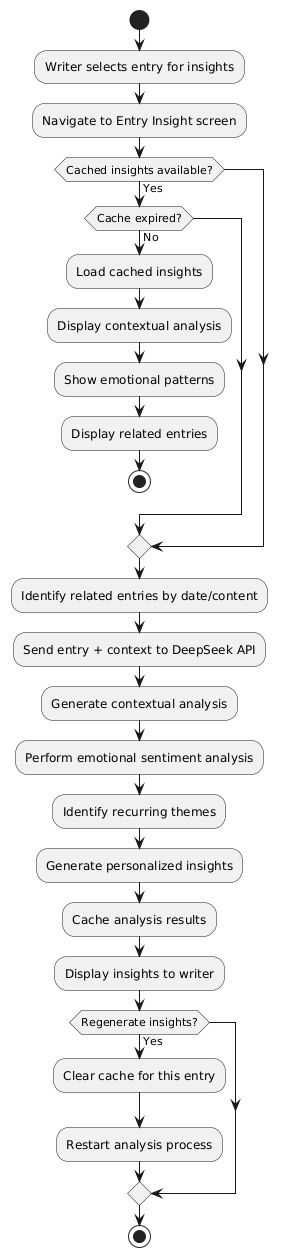
\includegraphics[width=0.95\textwidth,height=0.7\textheight,keepaspectratio]{files/imgs/insights_flow.png}
\caption{Insights flow for Writer}
\label{fig:insights-flow}
\end{figure}
\clearpage

\textbf{viii. Logout}

Figure~\ref{fig:logout-flow} shows the logout process for writers. The system securely terminates the user session, clears authentication tokens, and redirects to the login screen while ensuring local data remains protected.

\begin{figure}[H]
\centering
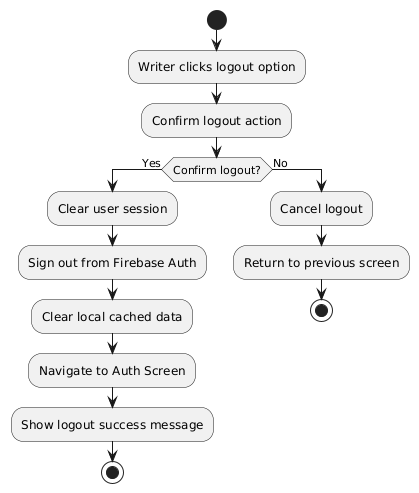
\includegraphics[width=0.95\textwidth,height=0.7\textheight,keepaspectratio]{files/imgs/logout_flow.png}
\caption{Logout flow for Writer}
\label{fig:logout-flow}
\end{figure}
\clearpage

\textbf{ix. Append Tags}

Figure~\ref{fig:append-tags-flow} shows the tag management flow. Writers can add, modify, or remove tags from their entries to improve organization and searchability. The system provides tag suggestions based on entry content and previous usage patterns.

\begin{figure}[H]
\centering
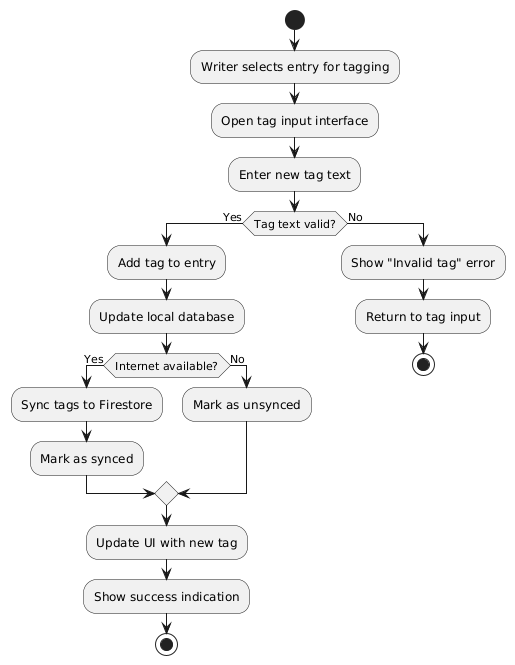
\includegraphics[width=0.95\textwidth,height=0.7\textheight,keepaspectratio]{files/imgs/append_tags_flow.png}
\caption{Append Tags flow for Writer}
\label{fig:append-tags-flow}
\end{figure}
\clearpage

\textbf{x. Set Mood}

Figure~\ref{fig:set-mood-flow} shows the mood setting functionality. Writers can associate emotional states with their entries, enabling the system to track emotional patterns over time and provide relevant insights.

\begin{figure}[H]
\centering
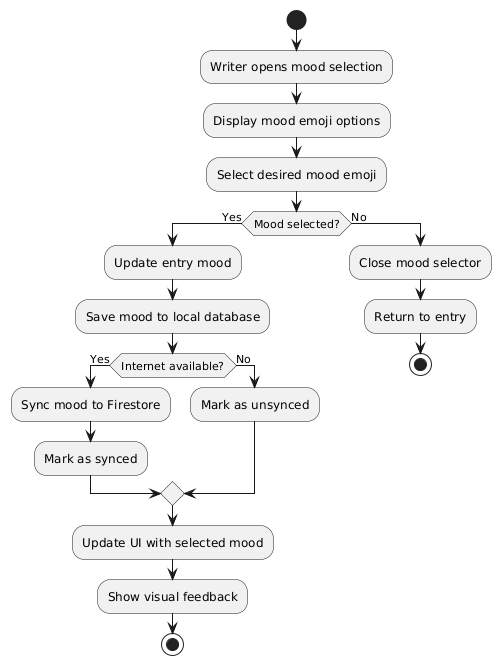
\includegraphics[width=0.95\textwidth,height=0.7\textheight,keepaspectratio]{files/imgs/set_mood_flow.png}
\caption{Set Mood flow for Writer}
\label{fig:set-mood-flow}
\end{figure}
\clearpage

\textbf{xi. Set Bookmark}

Figure~\ref{fig:set-bookmark-flow} shows the bookmarking process. Writers can mark important entries for quick access, creating a personalized collection of significant journal entries.

\begin{figure}[H]
\centering
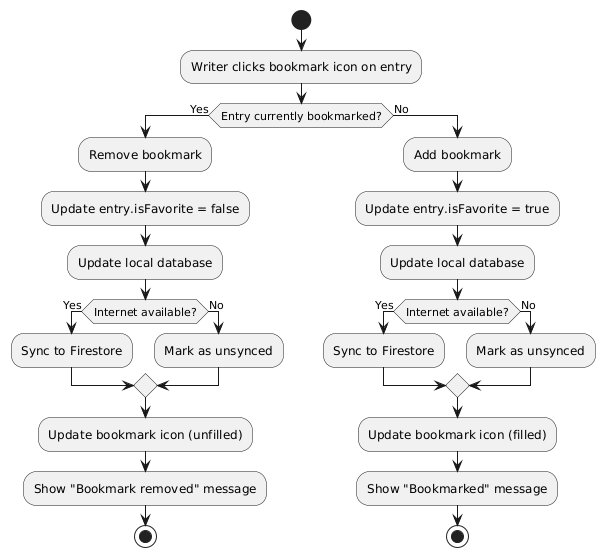
\includegraphics[width=0.95\textwidth,height=0.7\textheight,keepaspectratio]{files/imgs/set_bookmark_flow.png}
\caption{Set Bookmark flow for Writer}
\label{fig:set-bookmark-flow}
\end{figure}
\clearpage

\textbf{xii. Attach Media}

Figure~\ref{fig:attach-media-flow} shows the media attachment process. Writers can enhance their entries with images, GIFs, or other media content, with the system handling compression and storage optimization automatically.

\begin{figure}[H]
\centering
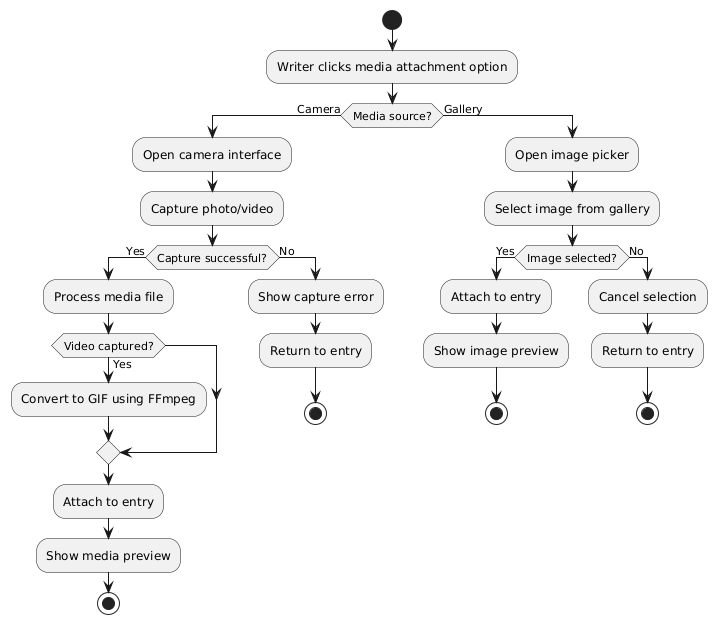
\includegraphics[width=0.95\textwidth,height=0.7\textheight,keepaspectratio]{files/imgs/attach_media_flow.png}
\caption{Attach Media flow for Writer}
\label{fig:attach-media-flow}
\end{figure}
\clearpage

\textbf{xiii. Browse Bookmark}

Figure~\ref{fig:browse-bookmark-flow} shows the bookmark browsing functionality. Writers can efficiently navigate through their bookmarked entries, with options for sorting and filtering based on various criteria.

\begin{figure}[H]
\centering
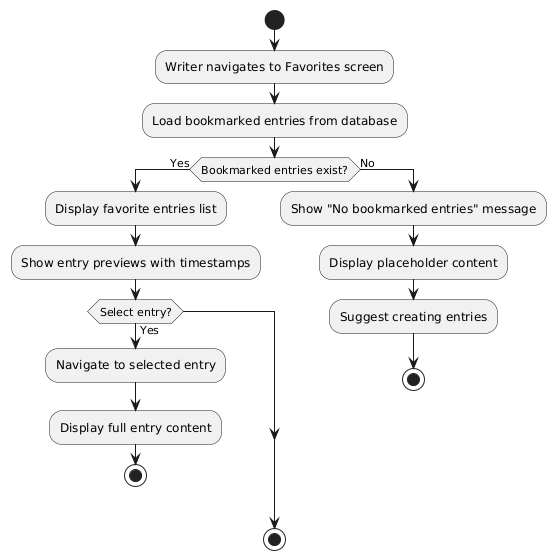
\includegraphics[width=0.95\textwidth,height=0.7\textheight,keepaspectratio]{files/imgs/browse_bookmark_flow.png}
\caption{Browse Bookmark flow for Writer}
\label{fig:browse-bookmark-flow}
\end{figure}
\clearpage

\textbf{xiv. View Entries}

Figure~\ref{fig:view-entries-flow} shows the entry viewing interface. Writers can browse through all their journal entries with various viewing options including list view, timeline view, and calendar integration.

\begin{figure}[H]
\centering
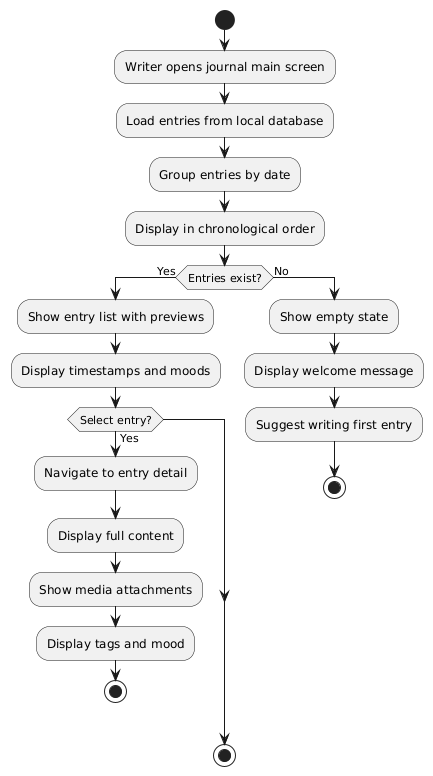
\includegraphics[width=0.95\textwidth,height=0.7\textheight,keepaspectratio]{files/imgs/view_entries_flow.png}
\caption{View Entries flow for Writer}
\label{fig:view-entries-flow}
\end{figure}
\clearpage

\textbf{xv. Browse Calendar}

Figure~\ref{fig:browse-calendar-flow} shows the calendar browsing functionality. Writers can navigate through their journaling history using an intuitive calendar interface, quickly jumping to entries from specific dates.

\begin{figure}[H]
\centering
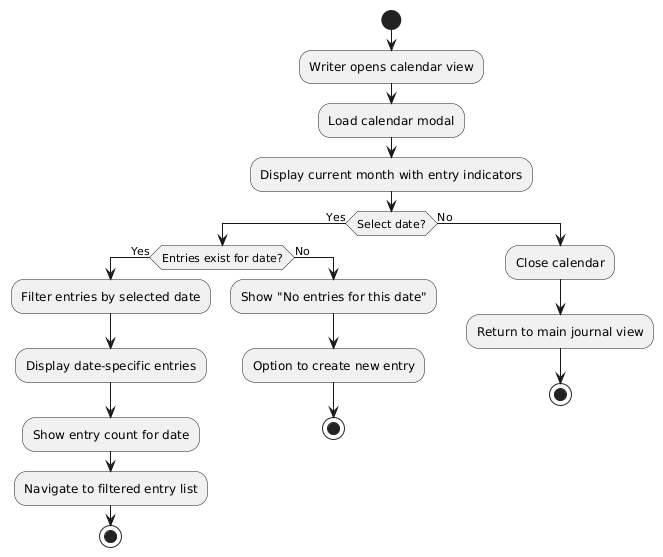
\includegraphics[width=0.95\textwidth,height=0.7\textheight,keepaspectratio]{files/imgs/browse_calendar_flow.png}
\caption{Browse Calendar flow for Writer}
\label{fig:browse-calendar-flow}
\end{figure}
\clearpage

\subsubsection{Backend Services}\label{subsubsec:backendServices}

This subsection covers the backend functionalities that support the user-facing features, including data management, synchronization, and AI processing capabilities.

\textbf{i. Store/Retrieve Entries}

Figure~\ref{fig:store-retrieve-entries-flow} shows the data management process for journal entries. The system handles secure storage and retrieval of entries across local and cloud storage, ensuring data integrity and availability.

\begin{figure}[H]
\centering
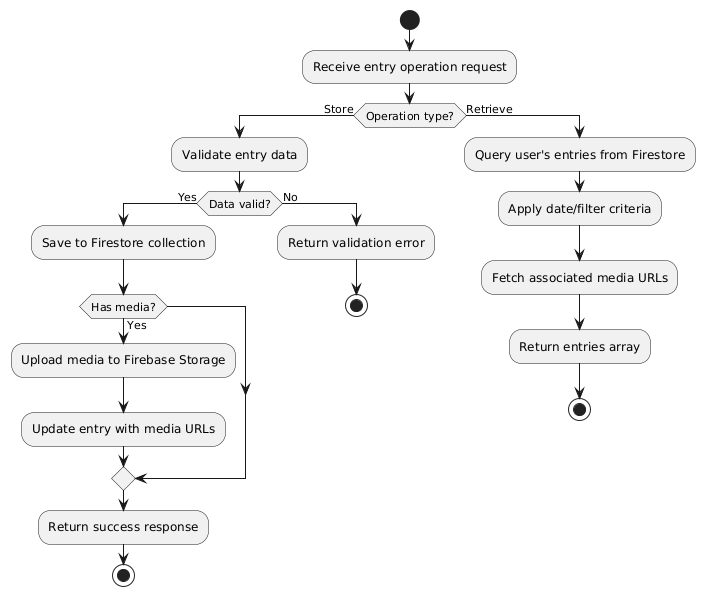
\includegraphics[width=0.8\textwidth]{files/imgs/store_retrieve_entries_flow.png}
\caption{Store/Retrieve Entries Flow}
\label{fig:store-retrieve-entries-flow}
\end{figure}
\clearpage

\textbf{ii. Manage Offline}

Figure~\ref{fig:manage-offline-flow} shows the offline functionality management. The system automatically handles offline mode, local data storage, and synchronization when connectivity is restored, ensuring seamless user experience regardless of network availability.

\begin{figure}[H]
\centering
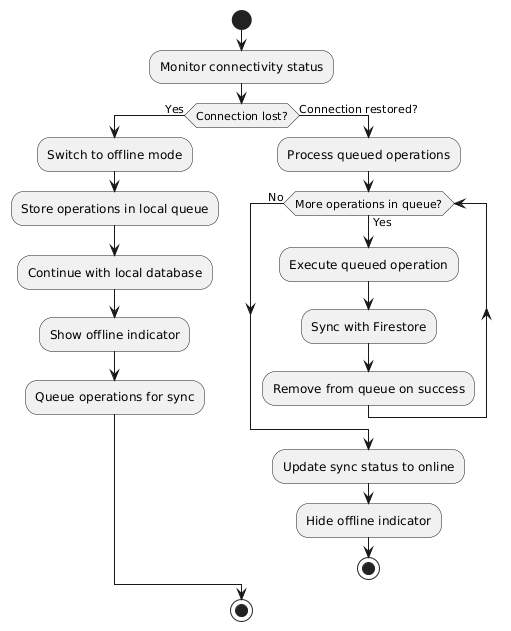
\includegraphics[width=0.8\textwidth]{files/imgs/manage_offline_flow.png}
\caption{Manage Offline Flow}
\label{fig:manage-offline-flow}
\end{figure}
\clearpage

\textbf{iii. Sync}

Figure~\ref{fig:sync-flow} shows the synchronization process between local and cloud storage. The system automatically detects connectivity changes and synchronizes data when internet access is available, maintaining data consistency across devices.

\begin{figure}[H]
\centering
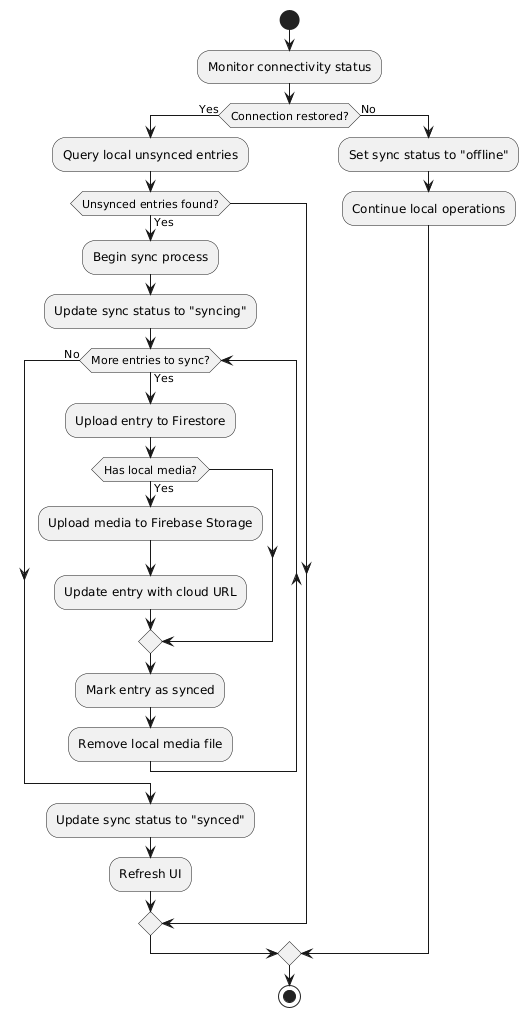
\includegraphics[width=0.95\textwidth,height=0.7\textheight,keepaspectratio]{files/imgs/sync_flow.png}
\caption{Synchronization Flow}
\label{fig:sync-flow}
\end{figure}
\clearpage

\textbf{iv. AI Processing}

Figure~\ref{fig:ai-processing-flow} shows the background AI processing that occurs automatically after entries are saved. The system performs sentiment analysis, pattern recognition, and insight generation without user intervention to maintain the simplicity of the journaling experience.

\begin{figure}[H]
\centering
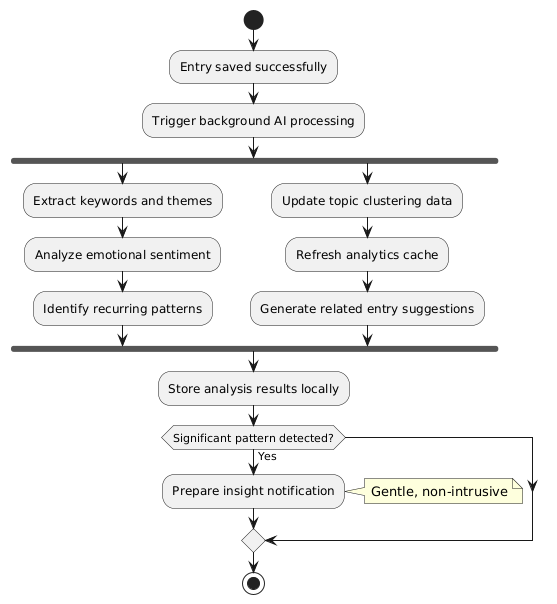
\includegraphics[width=0.8\textwidth]{files/imgs/ai_processing_flow.png}
\caption{AI Processing Flow}
\label{fig:ai-processing-flow}
\end{figure}
\clearpage

\subsection{Use Case}\label{subsec:useCase}

This subsection presents detailed use case analysis for the Collective mobile journaling application. Each use case includes a visual UML diagram and detailed specification table covering the use case ID, name, purpose, role, and various scenarios. The use cases are organized by functionality and provide comprehensive coverage of all system features available to writers.

\subsubsection{Register}

Figure~\ref{fig:usecase-register} shows the register use case diagram. This use case allows new users to create an account using email/password credentials or through OAuth providers like Google and Twitter/X.

\begin{figure}[H]
\centering
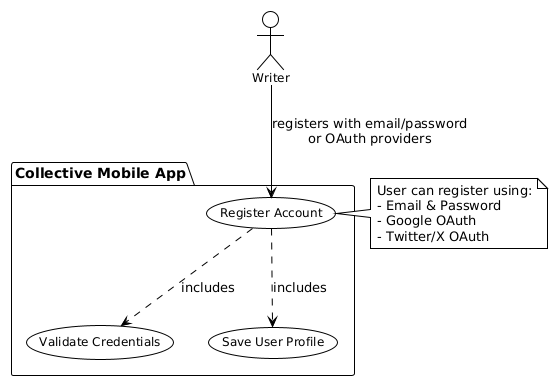
\includegraphics[width=0.8\textwidth]{files/imgs/usecase_U9ojKajF0Z.png}
\caption{Use Case Register}
\label{fig:usecase-register}
\end{figure}

\begin{table}[H]
\centering
\caption{Use Case Register Details}
\label{tab:usecase-register}
\begin{tabular}{|p{3cm}|p{11cm}|}
\hline
\textbf{Use Case ID} & UC-001 \\
\hline
\textbf{Use Case Name} & Register \\
\hline
\textbf{Purpose} & To allow writers to register a new account in the Collective application \\
\hline
\textbf{Role} & Writers \\
\hline
\textbf{Base Scenario} & 1. Writer opens the application for the first time \newline 2. Writer selects registration option \newline 3. Writer enters first name, last name, email, and password \newline 4. System validates the provided information \newline 5. System creates user profile in Firebase \newline 6. Writer is redirected to the main journal screen \\
\hline
\textbf{Alternative Scenario} & 1. Writer selects Google OAuth registration \newline 2. System redirects to Google authentication \newline 3. Writer authorizes the application \newline 4. System creates user profile using Google information \newline OR \newline 1. Writer selects Twitter/X OAuth registration \newline 2. System redirects to Twitter authentication \newline 3. Writer authorizes the application \newline 4. System creates user profile using Twitter information \\
\hline
\textbf{Exception Scenario} & 1. Email already exists in the system - System displays error message \newline 2. Invalid email format - System displays validation error \newline 3. Weak password - System requests stronger password \newline 4. Network connectivity issues - System displays retry option \newline 5. OAuth provider unavailable - System falls back to email registration \\
\hline
\end{tabular}
\end{table}

\subsubsection{Login}

Figure~\ref{fig:usecase-login} shows the login use case diagram. This use case enables existing users to authenticate and access their journal entries.

\begin{figure}[H]
\centering
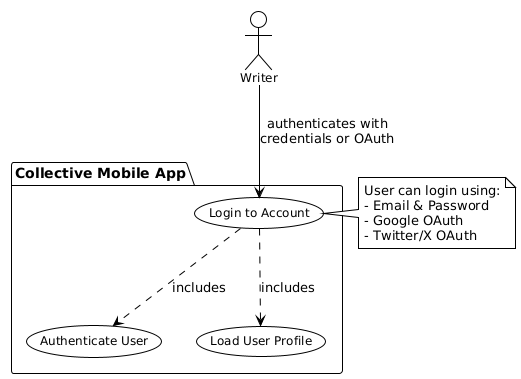
\includegraphics[width=0.8\textwidth]{files/imgs/usecase_U9ojKZrFmp.png}
\caption{Use Case Login}
\label{fig:usecase-login}
\end{figure}

\begin{table}[H]
\centering
\caption{Use Case Login Details}
\label{tab:usecase-login}
\begin{tabular}{|p{3cm}|p{11cm}|}
\hline
\textbf{Use Case ID} & UC-002 \\
\hline
\textbf{Use Case Name} & Login \\
\hline
\textbf{Purpose} & To allow writers to login into their existing account \\
\hline
\textbf{Role} & Writers \\
\hline
\textbf{Base Scenario} & 1. Writer opens the application \newline 2. Writer enters registered email and password \newline 3. System validates credentials against Firebase Authentication \newline 4. System loads user profile and preferences \newline 5. Writer is redirected to the main journal screen with access to their entries \\
\hline
\textbf{Alternative Scenario} & 1. Writer selects Google OAuth login \newline 2. System authenticates with Google services \newline 3. System validates existing account \newline 4. Writer gains immediate access to their journal \newline OR \newline 1. Writer selects Twitter/X OAuth login \newline 2. System authenticates with Twitter services \newline 3. System validates existing account \newline 4. Writer gains immediate access to their journal \\
\hline
\textbf{Exception Scenario} & 1. Incorrect email or password - System displays authentication error \newline 2. Account not found - System suggests registration \newline 3. Account temporarily locked - System displays wait message \newline 4. Network connectivity issues - System enables offline mode \newline 5. OAuth provider authentication fails - System provides alternative login methods \\
\hline
\end{tabular}
\end{table}

\subsubsection{Logout}

Figure~\ref{fig:usecase-logout} shows the logout use case diagram. This use case allows writers to securely terminate their session.

\begin{figure}[H]
\centering
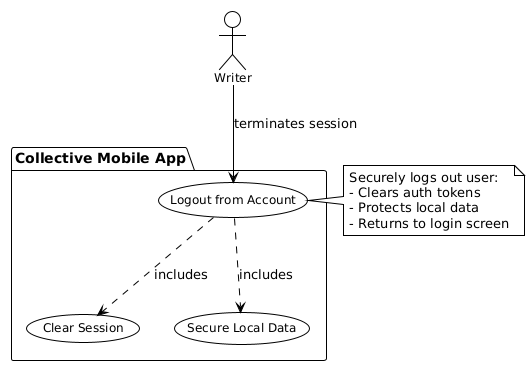
\includegraphics[width=0.8\textwidth]{files/imgs/usecase_U9ojaazFmp.png}
\caption{Use Case Logout}
\label{fig:usecase-logout}
\end{figure}

\begin{table}[H]
\centering
\caption{Use Case Logout Details}
\label{tab:usecase-logout}
\begin{tabular}{|p{3cm}|p{11cm}|}
\hline
\textbf{Use Case ID} & UC-003 \\
\hline
\textbf{Use Case Name} & Logout \\
\hline
\textbf{Purpose} & To allow writers to securely logout from their account \\
\hline
\textbf{Role} & Writers \\
\hline
\textbf{Base Scenario} & 1. Writer accesses logout option from the application menu \newline 2. System confirms logout intent \newline 3. System clears authentication tokens and session data \newline 4. System secures local data storage \newline 5. Writer is redirected to the login screen \\
\hline
\textbf{Alternative Scenario} & 1. Automatic logout due to session expiry \newline 2. System automatically clears session \newline 3. System displays session timeout message \newline 4. Writer is redirected to login screen \\
\hline
\textbf{Exception Scenario} & 1. Network issues during logout - System performs local logout and attempts sync later \newline 2. Unsaved data exists - System prompts to save before logout \newline 3. System error during logout - System forces local session termination \\
\hline
\end{tabular}
\end{table}

\subsubsection{Write Entry}

Figure~\ref{fig:usecase-write-entry} shows the write entry use case diagram. This core functionality allows writers to create new journal entries.

\begin{figure}[H]
\centering
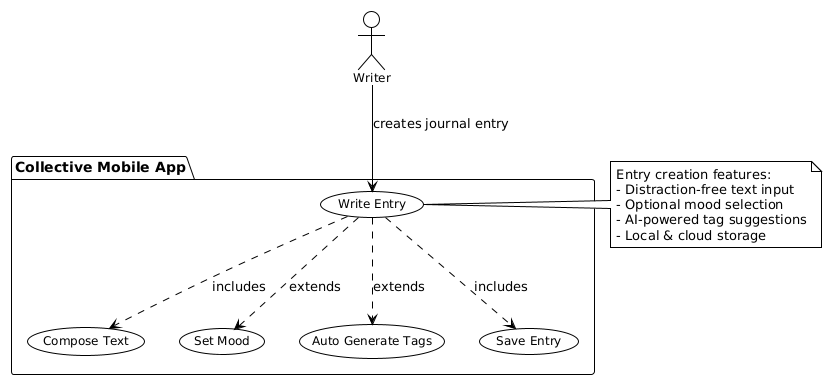
\includegraphics[width=0.8\textwidth]{files/imgs/usecase_U9ojKZjFmp.png}
\caption{Use Case Write Entry}
\label{fig:usecase-write-entry}
\end{figure}

\begin{table}[H]
\centering
\caption{Use Case Write Entry Details}
\label{tab:usecase-write-entry}
\begin{tabular}{|p{3cm}|p{11cm}|}
\hline
\textbf{Use Case ID} & UC-004 \\
\hline
\textbf{Use Case Name} & Write Entry \\
\hline
\textbf{Purpose} & To allow writers to create new journal entries with text, mood, and optional media \\
\hline
\textbf{Role} & Writers \\
\hline
\textbf{Base Scenario} & 1. Writer opens the journal input interface \newline 2. Writer composes their thoughts in the text area \newline 3. Writer optionally selects a mood from predefined options \newline 4. Writer optionally adds tags for organization \newline 5. Writer saves the entry using the save action \newline 6. System stores entry locally and syncs to cloud when available \\
\hline
\textbf{Alternative Scenario} & 1. Writer attaches an image to the entry \newline 2. System compresses and optimizes the media \newline 3. Writer continues with text composition \newline 4. System saves entry with media attachment \newline OR \newline 1. Writer creates entry while offline \newline 2. System saves entry to local database \newline 3. System queues entry for cloud sync when connectivity returns \\
\hline
\textbf{Exception Scenario} & 1. Empty entry attempted - System displays validation message \newline 2. Network failure during save - System saves locally and retries sync \newline 3. Storage space insufficient - System alerts user and suggests cleanup \newline 4. Image attachment too large - System compresses or requests smaller file \\
\hline
\end{tabular}
\end{table}

\subsubsection{Append Tags}

Figure~\ref{fig:usecase-append-tags} shows the append tags use case diagram. This functionality helps organize entries through tagging.

\begin{figure}[H]
\centering
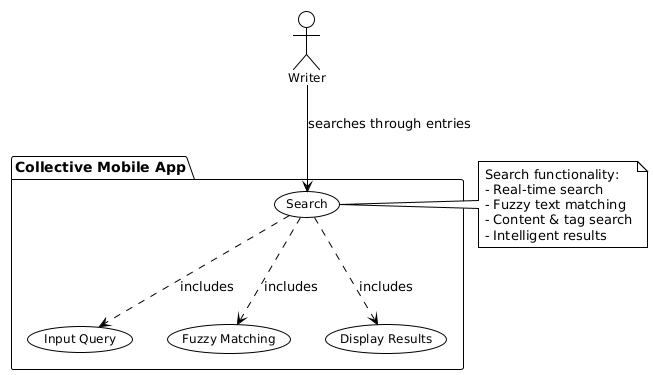
\includegraphics[width=0.8\textwidth]{files/imgs/usecase_U9ojKh5kmZ.png}
\caption{Use Case Append Tags}
\label{fig:usecase-append-tags}
\end{figure}

\begin{table}[H]
\centering
\caption{Use Case Append Tags Details}
\label{tab:usecase-append-tags}
\begin{tabular}{|p{3cm}|p{11cm}|}
\hline
\textbf{Use Case ID} & UC-005 \\
\hline
\textbf{Use Case Name} & Append Tags \\
\hline
\textbf{Purpose} & To allow writers to add organizational tags to their journal entries \\
\hline
\textbf{Role} & Writers \\
\hline
\textbf{Base Scenario} & 1. Writer accesses tag management for an entry \newline 2. System displays existing tags and suggestions \newline 3. Writer selects from suggested tags or creates custom tags \newline 4. Writer applies tags to the entry \newline 5. System updates entry metadata and improves future suggestions \\
\hline
\textbf{Alternative Scenario} & 1. AI system analyzes entry content \newline 2. System automatically suggests relevant tags \newline 3. Writer reviews and accepts/modifies suggestions \newline 4. System learns from writer preferences for future entries \\
\hline
\end{tabular}
\end{table}

\subsubsection{Set Mood}

Figure~\ref{fig:usecase-set-mood} shows the set mood use case diagram. This feature enables emotional tracking within entries.

\begin{figure}[H]
\centering
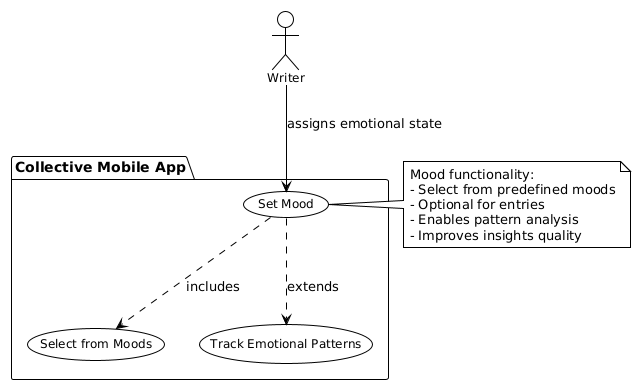
\includegraphics[width=0.8\textwidth]{files/imgs/usecase_U9ojKarFma.png}
\caption{Use Case Set Mood}
\label{fig:usecase-set-mood}
\end{figure}

\begin{table}[H]
\centering
\caption{Use Case Set Mood Details}
\label{tab:usecase-set-mood}
\begin{tabular}{|p{3cm}|p{11cm}|}
\hline
\textbf{Use Case ID} & UC-006 \\
\hline
\textbf{Use Case Name} & Set Mood \\
\hline
\textbf{Purpose} & To allow writers to associate emotional states with their journal entries \\
\hline
\textbf{Role} & Writers \\
\hline
\textbf{Base Scenario} & 1. Writer accesses mood selection interface during entry creation \newline 2. System displays predefined mood options (happy, sad, anxious, etc.) \newline 3. Writer selects the mood that best represents their emotional state \newline 4. System associates the mood with the entry for pattern analysis \newline 5. System updates emotional tracking data for analytics \\
\hline
\textbf{Alternative Scenario} & 1. Writer chooses not to set a mood (optional feature) \newline 2. System saves entry without mood association \newline 3. Entry remains available for mood addition later \newline OR \newline 1. Writer changes mood after initial entry creation \newline 2. System updates mood association \newline 3. System recalculates emotional patterns if needed \\
\hline
\textbf{Exception Scenario} & 1. Mood data inconsistency - System uses default neutral mood \newline 2. Multiple mood selections attempted - System uses last selection \newline 3. Invalid mood data - System prompts for re-selection \\
\hline
\end{tabular}
\end{table}

\subsubsection{Set Bookmark}

Figure~\ref{fig:usecase-set-bookmark} shows the set bookmark use case diagram. This feature allows writers to mark important entries.

\begin{figure}[H]
\centering
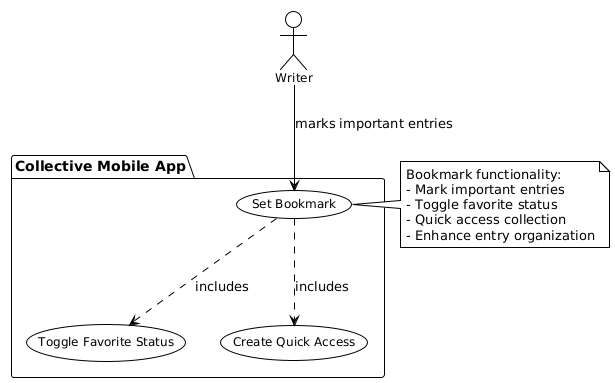
\includegraphics[width=0.8\textwidth]{files/imgs/usecase_U9ojaZzlWp.png}
\caption{Use Case Set Bookmark}
\label{fig:usecase-set-bookmark}
\end{figure}

\begin{table}[H]
\centering
\caption{Use Case Set Bookmark Details}
\label{tab:usecase-set-bookmark}
\begin{tabular}{|p{3cm}|p{11cm}|}
\hline
\textbf{Use Case ID} & UC-007 \\
\hline
\textbf{Use Case Name} & Set Bookmark \\
\hline
\textbf{Purpose} & To allow writers to bookmark important entries for quick access \\
\hline
\textbf{Role} & Writers \\
\hline
\textbf{Base Scenario} & 1. Writer identifies an important entry to bookmark \newline 2. Writer selects the bookmark/favorite option \newline 3. System toggles the bookmark status of the entry \newline 4. System updates the entry metadata \newline 5. Entry becomes accessible through the favorites collection \\
\hline
\textbf{Alternative Scenario} & 1. Writer removes bookmark from previously bookmarked entry \newline 2. System toggles bookmark status to off \newline 3. Entry is removed from favorites collection but remains in main timeline \\
\hline
\textbf{Exception Scenario} & 1. Bookmark data corruption - System resets bookmark status \newline 2. Sync conflict with bookmark status - System uses most recent version \newline 3. Maximum bookmarks reached - System displays limit notification \\
\hline
\end{tabular}
\end{table}

\subsubsection{Attach Media}

Figure~\ref{fig:usecase-attach-media} shows the attach media use case diagram. This functionality enhances entries with visual content.

\begin{figure}[H]
\centering
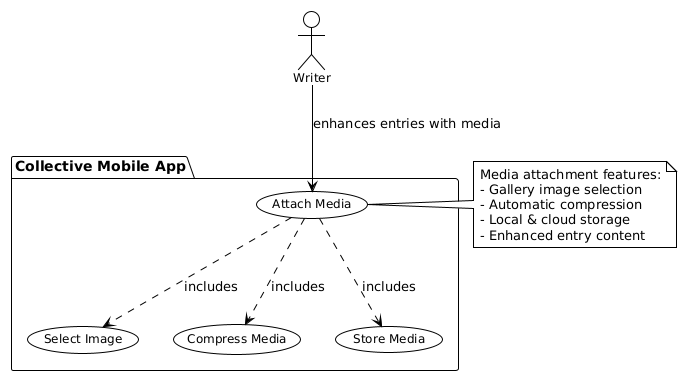
\includegraphics[width=0.8\textwidth]{files/imgs/usecase_U9ojKZjhmp.png}
\caption{Use Case Attach Media}
\label{fig:usecase-attach-media}
\end{figure}

\begin{table}[H]
\centering
\caption{Use Case Attach Media Details}
\label{tab:usecase-attach-media}
\begin{tabular}{|p{3cm}|p{11cm}|}
\hline
\textbf{Use Case ID} & UC-008 \\
\hline
\textbf{Use Case Name} & Attach Media \\
\hline
\textbf{Purpose} & To allow writers to enhance their entries with images and media content \\
\hline
\textbf{Role} & Writers \\
\hline
\textbf{Base Scenario} & 1. Writer selects media attachment option during entry creation \newline 2. System opens device gallery or camera interface \newline 3. Writer selects or captures an image \newline 4. System compresses and optimizes the media file \newline 5. System associates media with the entry and stores locally \newline 6. System uploads media to cloud storage when connectivity available \\
\hline
\textbf{Alternative Scenario} & 1. Writer attaches multiple images to single entry \newline 2. System processes each image individually \newline 3. System creates media gallery for the entry \newline OR \newline 1. Writer removes attached media \newline 2. System removes media association and files \newline 3. System updates entry metadata \\
\hline
\textbf{Exception Scenario} & 1. Image file too large - System compresses or requests smaller file \newline 2. Unsupported file format - System displays supported format message \newline 3. Storage space insufficient - System alerts and suggests cleanup \newline 4. Upload failure - System retries upload when connectivity restored \newline 5. Corrupted media file - System displays error and removes attachment \\
\hline
\end{tabular}
\end{table}

\subsubsection{Submit Entry}

Figure~\ref{fig:usecase-submit-entry} shows the submit entry use case diagram. This finalizes the entry creation process.

\begin{figure}[H]
\centering
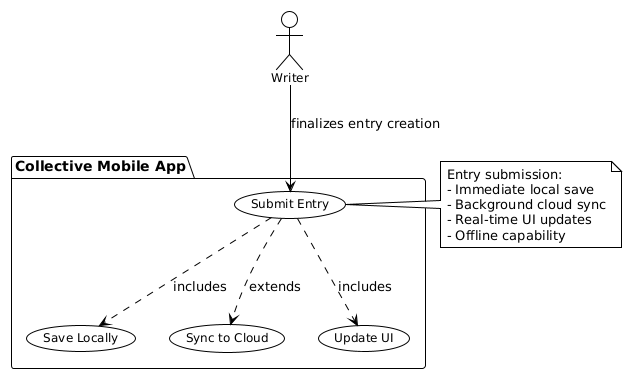
\includegraphics[width=0.8\textwidth]{files/imgs/usecase_U9ojaa5Fmp.png}
\caption{Use Case Submit Entry}
\label{fig:usecase-submit-entry}
\end{figure}

\begin{table}[H]
\centering
\caption{Use Case Submit Entry Details}
\label{tab:usecase-submit-entry}
\begin{tabular}{|p{3cm}|p{11cm}|}
\hline
\textbf{Use Case ID} & UC-009 \\
\hline
\textbf{Use Case Name} & Submit Entry \\
\hline
\textbf{Purpose} & To allow writers to finalize and save their completed journal entries \\
\hline
\textbf{Role} & Writers \\
\hline
\textbf{Base Scenario} & 1. Writer completes entry composition with text, mood, tags, and media \newline 2. Writer selects save/submit action \newline 3. System validates entry content and metadata \newline 4. System saves entry to local database immediately \newline 5. System updates UI to reflect new entry \newline 6. System queues entry for cloud synchronization \\
\hline
\textbf{Alternative Scenario} & 1. Auto-save triggers during entry composition \newline 2. System saves draft entry periodically \newline 3. Writer can continue editing or finalize submission \newline OR \newline 1. Writer submits entry while offline \newline 2. System saves locally with sync pending status \newline 3. System syncs when connectivity restored \\
\hline
\textbf{Exception Scenario} & 1. Entry validation fails - System highlights issues and prevents submission \newline 2. Local storage full - System displays storage warning \newline 3. Duplicate entry detected - System asks for confirmation \newline 4. System crash during submission - System recovers draft on restart \\
\hline
\end{tabular}
\end{table}

\subsubsection{Browse Bookmark}

Figure~\ref{fig:usecase-browse-bookmark} shows the browse bookmark use case diagram. This provides access to favorite entries.

\begin{figure}[H]
\centering
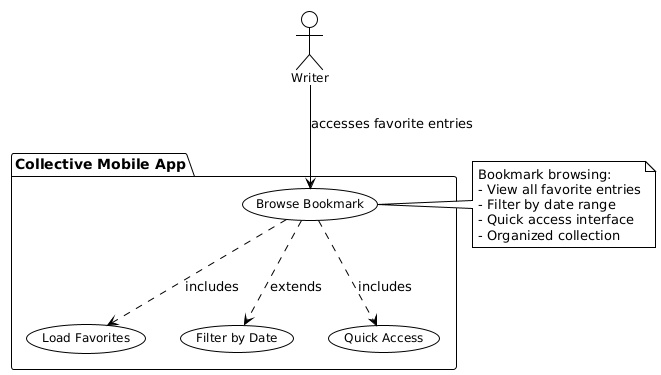
\includegraphics[width=0.8\textwidth]{files/imgs/usecase_U9ojaarlmZ.png}
\caption{Use Case Browse Bookmark}
\label{fig:usecase-browse-bookmark}
\end{figure}

\begin{table}[H]
\centering
\caption{Use Case Browse Bookmark Details}
\label{tab:usecase-browse-bookmark}
\begin{tabular}{|p{3cm}|p{11cm}|}
\hline
\textbf{Use Case ID} & UC-010 \\
\hline
\textbf{Use Case Name} & Browse Bookmark \\
\hline
\textbf{Purpose} & To allow writers to access and browse their bookmarked/favorite entries \\
\hline
\textbf{Role} & Writers \\
\hline
\textbf{Base Scenario} & 1. Writer accesses the favorites/bookmarks section \newline 2. System loads all bookmarked entries \newline 3. System displays entries in chronological or custom order \newline 4. Writer can browse, read, edit, or remove bookmarks \newline 5. Writer can access full entry details and associated media \\
\hline
\textbf{Alternative Scenario} & 1. Writer applies date range filter to bookmarks \newline 2. System filters bookmarked entries by specified dates \newline 3. System displays filtered results \newline OR \newline 1. Writer searches within bookmarked entries \newline 2. System performs search only within favorite entries \newline 3. System displays matching bookmarked entries \\
\hline
\textbf{Exception Scenario} & 1. No bookmarked entries exist - System displays empty state with guidance \newline 2. Bookmark data corrupted - System attempts recovery or resets bookmarks \newline 3. Loading error - System displays retry option \newline 4. Network issues - System shows cached bookmarks with sync status \\
\hline
\end{tabular}
\end{table}

\subsubsection{View Entries}

Figure~\ref{fig:usecase-view-entries} shows the view entries use case diagram. This provides the main interface for browsing all journal entries.

\begin{figure}[H]
\centering
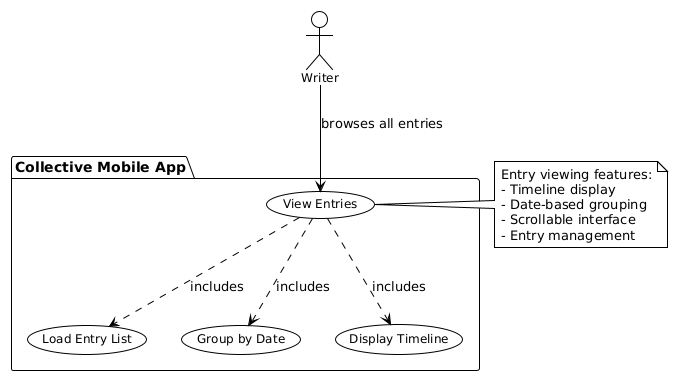
\includegraphics[width=0.8\textwidth]{files/imgs/usecase_U9ojah5omZ.png}
\caption{Use Case View Entries}
\label{fig:usecase-view-entries}
\end{figure}

\begin{table}[H]
\centering
\caption{Use Case View Entries Details}
\label{tab:usecase-view-entries}
\begin{tabular}{|p{3cm}|p{11cm}|}
\hline
\textbf{Use Case ID} & UC-011 \\
\hline
\textbf{Use Case Name} & View Entries \\
\hline
\textbf{Purpose} & To allow writers to browse and view all their journal entries in an organized timeline \\
\hline
\textbf{Role} & Writers \\
\hline
\textbf{Base Scenario} & 1. Writer opens the main journal screen \newline 2. System loads all journal entries from local and cloud storage \newline 3. System groups entries by date for organized display \newline 4. System displays entries in reverse chronological order \newline 5. Writer can scroll through timeline and access individual entries \\
\hline
\textbf{Alternative Scenario} & 1. Writer filters entries by date range \newline 2. System displays entries within specified timeframe \newline OR \newline 1. Writer sorts entries by different criteria (mood, tags, etc.) \newline 2. System reorganizes display according to selected sorting \\
\hline
\textbf{Exception Scenario} & 1. No entries exist - System displays welcome message and entry creation guidance \newline 2. Loading error - System shows cached entries with sync status indicator \newline 3. Large number of entries causes performance issues - System implements pagination \newline 4. Data corruption detected - System attempts recovery and shows error status \\
\hline
\end{tabular}
\end{table}

\subsubsection{Search}

Figure~\ref{fig:usecase-search} shows the search use case diagram. This enables efficient entry discovery through text matching.

\begin{figure}[H]
\centering
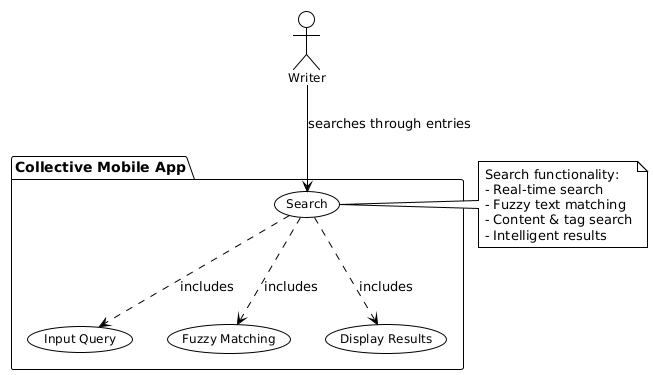
\includegraphics[width=0.8\textwidth]{files/imgs/usecase_U9ojKh5kmZ.png}
\caption{Use Case Search}
\label{fig:usecase-search}
\end{figure}

\begin{table}[H]
\centering
\caption{Use Case Search Details}
\label{tab:usecase-search}
\begin{tabular}{|p{3cm}|p{11cm}|}
\hline
\textbf{Use Case ID} & UC-012 \\
\hline
\textbf{Use Case Name} & Search \\
\hline
\textbf{Purpose} & To allow writers to search through their journal entries using keywords and phrases \\
\hline
\textbf{Role} & Writers \\
\hline
\textbf{Base Scenario} & 1. Writer activates search interface \newline 2. Writer enters search keywords or phrases \newline 3. System performs real-time fuzzy text matching across entry content and tags \newline 4. System displays matching entries with highlighted search terms \newline 5. Writer can access full entries from search results \\
\hline
\textbf{Alternative Scenario} & 1. Writer searches by specific tags \newline 2. System filters entries containing specified tags \newline 3. System displays tag-filtered results \newline OR \newline 1. Writer uses advanced search with multiple criteria \newline 2. System combines text, tag, mood, and date filters \newline 3. System displays comprehensive filtered results \\
\hline
\textbf{Exception Scenario} & 1. No search results found - System displays no results message with search suggestions \newline 2. Search query too short - System requires minimum character count \newline 3. Special characters in search - System sanitizes query and searches \newline 4. Search performance issues - System optimizes query and displays progress indicator \\
\hline
\end{tabular}
\end{table}

\subsubsection{Browse Calendar}

Figure~\ref{fig:usecase-browse-calendar} shows the browse calendar use case diagram. This provides date-based navigation through entries.

\begin{figure}[H]
\centering
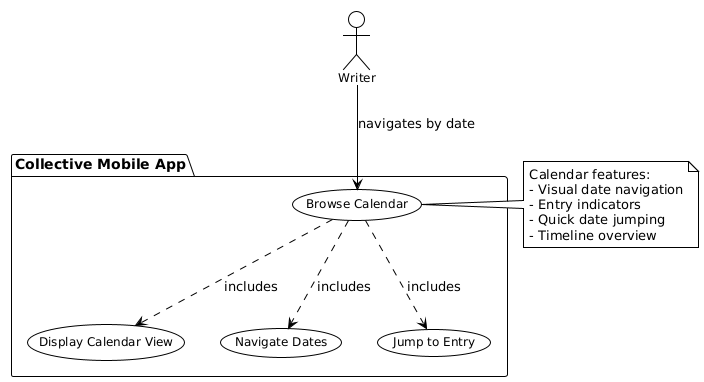
\includegraphics[width=0.8\textwidth]{files/imgs/usecase_U9ojaarFma.png}
\caption{Use Case Browse Calendar}
\label{fig:usecase-browse-calendar}
\end{figure}

\begin{table}[H]
\centering
\caption{Use Case Browse Calendar Details}
\label{tab:usecase-browse-calendar}
\begin{tabular}{|p{3cm}|p{11cm}|}
\hline
\textbf{Use Case ID} & UC-013 \\
\hline
\textbf{Use Case Name} & Browse Calendar \\
\hline
\textbf{Purpose} & To allow writers to navigate their journal entries using a visual calendar interface \\
\hline
\textbf{Role} & Writers \\
\hline
\textbf{Base Scenario} & 1. Writer accesses calendar view from main interface \newline 2. System displays calendar with entry indicators on dates with journal entries \newline 3. Writer navigates through months and years \newline 4. Writer selects specific date with entries \newline 5. System navigates to entries for selected date in main timeline \\
\hline
\textbf{Alternative Scenario} & 1. Writer uses calendar to find entries from specific time period \newline 2. System highlights date ranges with entry activity \newline 3. Writer selects date range for filtered viewing \newline OR \newline 1. Calendar displays mood indicators for each date \newline 2. Writer can visualize emotional patterns over time \newline 3. Writer selects dates based on mood indicators \\
\hline
\textbf{Exception Scenario} & 1. Calendar fails to load - System displays alternative date navigation \newline 2. Date with no entries selected - System offers to create new entry for that date \newline 3. Performance issues with large date ranges - System implements lazy loading \newline 4. Invalid date selection - System corrects to nearest valid date \\
\hline
\end{tabular}
\end{table}

\subsubsection{View Analytics}

Figure~\ref{fig:usecase-view-analytics} shows the view analytics use case diagram. This provides insights into journaling patterns and trends.

\begin{figure}[H]
\centering
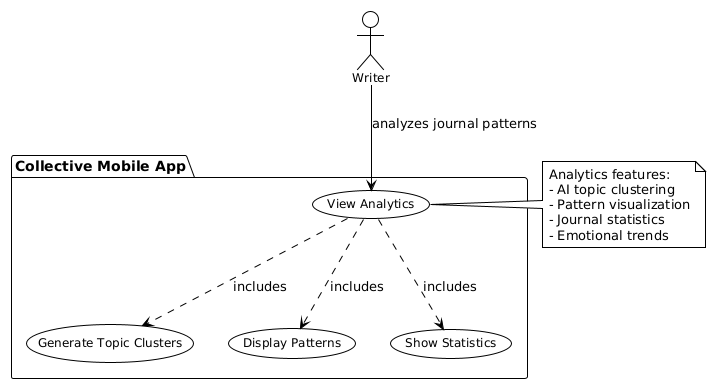
\includegraphics[width=0.8\textwidth]{files/imgs/usecase_U9ojaijEmp.png}
\caption{Use Case View Analytics}
\label{fig:usecase-view-analytics}
\end{figure}

\begin{table}[H]
\centering
\caption{Use Case View Analytics Details}
\label{tab:usecase-view-analytics}
\begin{tabular}{|p{3cm}|p{11cm}|}
\hline
\textbf{Use Case ID} & UC-014 \\
\hline
\textbf{Use Case Name} & View Analytics \\
\hline
\textbf{Purpose} & To allow writers to analyze their journaling patterns, topics, and emotional trends \\
\hline
\textbf{Role} & Writers \\
\hline
\textbf{Base Scenario} & 1. Writer accesses analytics section from main interface \newline 2. System analyzes journal entries to identify topic clusters and patterns \newline 3. System generates visualizations showing topic distribution and trends \newline 4. System displays emotional patterns and mood statistics \newline 5. Writer can explore individual topic clusters and associated entries \\
\hline
\textbf{Alternative Scenario} & 1. System uses cached analytics when available \newline 2. System displays previously generated insights immediately \newline 3. System updates analytics in background when new entries added \newline OR \newline 1. Writer requests analytics refresh \newline 2. System regenerates analysis with current data \newline 3. System displays updated insights and patterns \\
\hline
\textbf{Exception Scenario} & 1. Insufficient data for analytics - System displays message about minimum entry requirements \newline 2. Analytics generation fails - System displays error and retry option \newline 3. Complex analytics take too long - System displays progress and allows backgrounding \newline 4. Analytics data corrupted - System regenerates from source entries \\
\hline
\end{tabular}
\end{table}

\subsubsection{View AI Insights}

Figure~\ref{fig:usecase-view-ai-insights} shows the view AI insights use case diagram. This provides detailed AI-powered analysis of individual entries.

\begin{figure}[H]
\centering
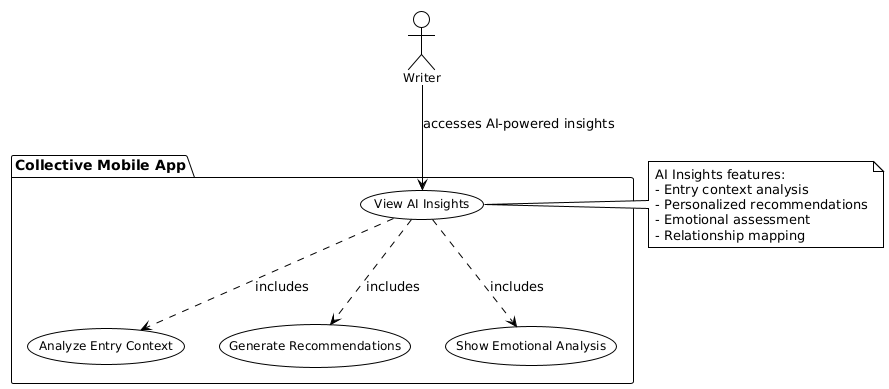
\includegraphics[width=0.8\textwidth]{files/imgs/usecase_U9ojKijEmp.png}
\caption{Use Case View AI Insights}
\label{fig:usecase-view-ai-insights}
\end{figure}

\begin{table}[H]
\centering
\caption{Use Case View AI Insights Details}
\label{tab:usecase-view-ai-insights}
\begin{tabular}{|p{3cm}|p{11cm}|}
\hline
\textbf{Use Case ID} & UC-015 \\
\hline
\textbf{Use Case Name} & View AI Insights \\
\hline
\textbf{Purpose} & To allow writers to access AI-powered insights and analysis for individual journal entries \\
\hline
\textbf{Role} & Writers \\
\hline
\textbf{Base Scenario} & 1. Writer selects AI insights option for a specific entry \newline 2. System analyzes entry content using AI services \newline 3. System generates contextual insights about themes, emotions, and relationships \newline 4. System provides personalized recommendations based on entry content \newline 5. Writer reviews insights and can apply suggestions to future entries \\
\hline
\textbf{Alternative Scenario} & 1. System displays cached insights if previously generated \newline 2. System shows processing status for new analysis \newline 3. System updates insights when analysis completes \newline OR \newline 1. Writer requests insight regeneration \newline 2. System reprocesses entry with updated AI models \newline 3. System displays refreshed insights and recommendations \\
\hline
\textbf{Exception Scenario} & 1. AI service unavailable - System displays cached insights or error message \newline 2. Entry too short for analysis - System suggests minimum content requirements \newline 3. Analysis fails - System provides basic insights and retry option \newline 4. Rate limiting from AI service - System queues analysis for later processing \\
\hline
\end{tabular}
\end{table}

\subsubsection{Manage Offline}

Figure~\ref{fig:usecase-manage-offline} shows the manage offline use case diagram. This ensures functionality without internet connectivity.

\begin{figure}[H]
\centering
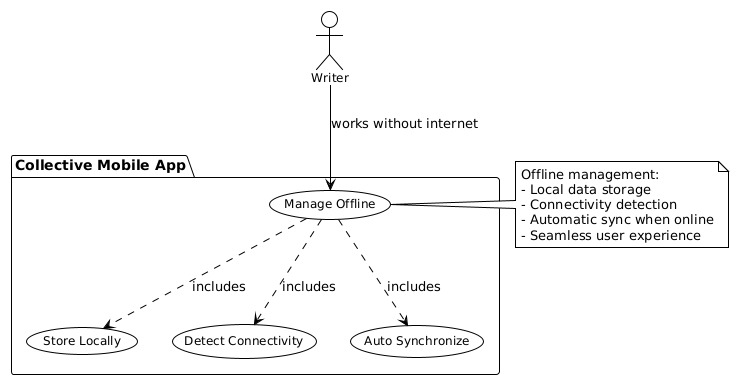
\includegraphics[width=0.8\textwidth]{files/imgs/usecase_U9ojaa5Fma.png}
\caption{Use Case Manage Offline}
\label{fig:usecase-manage-offline}
\end{figure}

\begin{table}[H]
\centering
\caption{Use Case Manage Offline Details}
\label{tab:usecase-manage-offline}
\begin{tabular}{|p{3cm}|p{11cm}|}
\hline
\textbf{Use Case ID} & UC-016 \\
\hline
\textbf{Use Case Name} & Manage Offline \\
\hline
\textbf{Purpose} & To allow writers to use the application fully when internet connectivity is unavailable \\
\hline
\textbf{Role} & Writers \\
\hline
\textbf{Base Scenario} & 1. System detects loss of internet connectivity \newline 2. System switches to offline mode seamlessly \newline 3. System stores all new entries and changes locally \newline 4. System provides full functionality using local database \newline 5. System detects connectivity restoration and synchronizes changes \\
\hline
\textbf{Alternative Scenario} & 1. User manually enables offline mode \newline 2. System prepares for offline operation \newline 3. System caches essential data locally \newline OR \newline 1. Partial connectivity available \newline 2. System optimizes for low-bandwidth operation \newline 3. System prioritizes essential sync operations \\
\hline
\textbf{Exception Scenario} & 1. Local storage insufficient for offline data - System alerts user and suggests cleanup \newline 2. Sync conflicts when connectivity restored - System provides conflict resolution interface \newline 3. Local database corruption - System attempts recovery and alerts user \newline 4. Extended offline period - System optimizes local storage and manages capacity \\
\hline
\end{tabular}
\end{table}

\subsubsection{Generate Analytics}

Figure~\ref{fig:usecase-generate-analytics} shows the generate analytics use case diagram. This backend process creates analytical insights from journal data.

\begin{figure}[H]
\centering
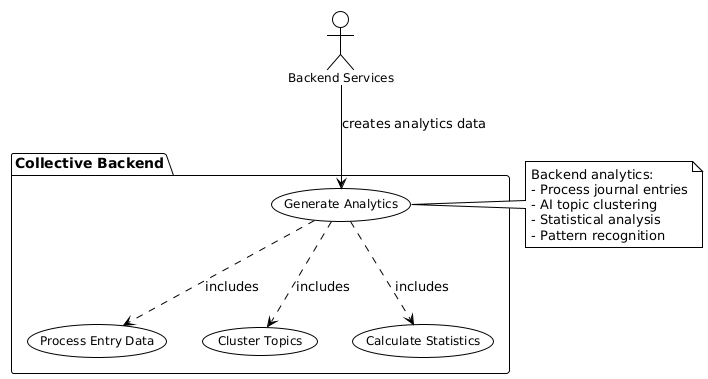
\includegraphics[width=0.8\textwidth]{files/imgs/usecase_U9ojaazhma.png}
\caption{Use Case Generate Analytics}
\label{fig:usecase-generate-analytics}
\end{figure}

\begin{table}[H]
\centering
\caption{Use Case Generate Analytics Details}
\label{tab:usecase-generate-analytics}
\begin{tabular}{|p{3cm}|p{11cm}|}
\hline
\textbf{Use Case ID} & UC-017 \\
\hline
\textbf{Use Case Name} & Generate Analytics \\
\hline
\textbf{Purpose} & To process journal entries and generate analytical insights, patterns, and statistics \\
\hline
\textbf{Role} & Backend Services \\
\hline
\textbf{Base Scenario} & 1. System receives request for analytics generation \newline 2. System processes all available journal entries \newline 3. System applies AI algorithms to identify topic clusters \newline 4. System calculates statistical patterns and trends \newline 5. System stores generated analytics for user access \newline 6. System caches results for improved performance \\
\hline
\textbf{Alternative Scenario} & 1. System performs incremental analytics update \newline 2. System processes only new entries since last analysis \newline 3. System updates existing analytics with new patterns \newline OR \newline 1. System runs scheduled background analytics \newline 2. System automatically updates insights for active users \newline 3. System optimizes processing for system resources \\
\hline
\textbf{Exception Scenario} & 1. Insufficient data for meaningful analytics - System provides guidance on minimum requirements \newline 2. Processing timeout due to large dataset - System implements chunked processing \newline 3. AI service unavailable - System falls back to basic statistical analysis \newline 4. Memory or processing constraints - System optimizes algorithms and processes in batches \\
\hline
\end{tabular}
\end{table}

\subsubsection{Generate Insights}

Figure~\ref{fig:usecase-generate-insights} shows the generate insights use case diagram. This backend process creates personalized AI insights for individual entries.

\begin{figure}[H]
\centering
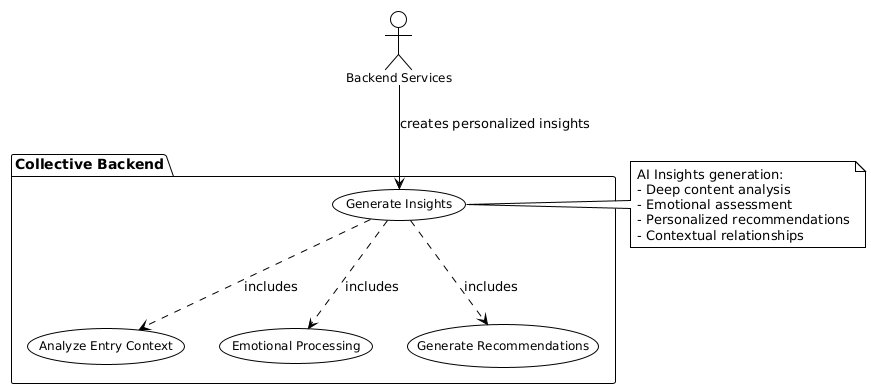
\includegraphics[width=0.8\textwidth]{files/imgs/usecase_U9ojKijkmZ.png}
\caption{Use Case Generate Insights}
\label{fig:usecase-generate-insights}
\end{figure}

\begin{table}[H]
\centering
\caption{Use Case Generate Insights Details}
\label{tab:usecase-generate-insights}
\begin{tabular}{|p{3cm}|p{11cm}|}
\hline
\textbf{Use Case ID} & UC-018 \\
\hline
\textbf{Use Case Name} & Generate Insights \\
\hline
\textbf{Purpose} & To create personalized AI-powered insights and recommendations for individual journal entries \\
\hline
\textbf{Role} & Backend Services \\
\hline
\textbf{Base Scenario} & 1. System receives request for entry-specific insight generation \newline 2. System analyzes entry content using natural language processing \newline 3. System performs emotional and contextual analysis \newline 4. System generates personalized recommendations and insights \newline 5. System stores insights linked to specific entry \newline 6. System provides insights to user interface \\
\hline
\textbf{Alternative Scenario} & 1. System uses historical user data to enhance insights \newline 2. System considers user's journaling patterns and preferences \newline 3. System provides more personalized and relevant recommendations \newline OR \newline 1. System batches multiple entries for efficient processing \newline 2. System generates insights for multiple entries simultaneously \newline 3. System optimizes AI service usage and costs \\
\hline
\textbf{Exception Scenario} & 1. AI service rate limiting - System queues requests and processes when capacity available \newline 2. Entry content insufficient for analysis - System provides general insights and suggestions \newline 3. Processing failure - System logs error and provides retry mechanism \newline 4. User privacy restrictions - System processes locally or uses anonymized analysis \\
\hline
\end{tabular}
\end{table}

\subsection{Product Functions}\label{subsec:productFunctions}

This section presents a comprehensive overview of the functional requirements for the \textbf{Collective} mobile journaling application. Each function is detailed with a unique identifier, feature name, description, and accessible user role. The functions are organized by categories covering authentication, journaling core features, content management, AI-powered features, and system utilities. Table~\ref{tab:function-summary} provides an overview of all 31 functional requirements.

\begin{table}[H]
\centering
\caption{Functional Requirements Summary}
\label{tab:function-summary}
\begin{tabular}{|p{2.5cm}|p{3cm}|p{7.5cm}|}
\hline
\textbf{Category} & \textbf{Function Range} & \textbf{Description} \\
\hline
Authentication & F001 - F003 & User registration, login, and logout functionality \\
\hline
Core Journaling & F004 - F007 & Entry creation, editing, deletion, and submission \\
\hline
Content Enhancement & F008 - F011 & Mood setting, tagging, media attachment, bookmarking \\
\hline
Content Management & F012 - F015 & Entry viewing, searching, calendar browsing, bookmark management \\
\hline
AI Analysis & F016 - F019 & AI insights generation and analytics viewing \\
\hline
Data Management & F020 - F023 & Data storage, retrieval, offline management, synchronization \\
\hline
User Interface & F024 - F027 & Selection modes, themes, responsive design, progress feedback \\
\hline
System Utilities & F028 - F031 & Error handling, validation, performance, security \\
\hline
\end{tabular}
\end{table}

\newpage

\subsubsection{Authentication and User Management Functions}

The authentication system provides secure user access control with multiple authentication methods. These functions ensure user identity verification and session management.

\begin{table}[H]
\centering
\caption{Authentication Functions}
\label{tab:auth-functions}
\begin{tabular}{|p{0.8cm}|p{2.2cm}|p{9.5cm}|p{1.5cm}|}
\hline
\textbf{ID} & \textbf{Function} & \textbf{Description} & \textbf{Role} \\
\hline
F001 & Register & Allow new users to create accounts using email/password, Google OAuth, or Twitter/X OAuth with validation and secure profile creation & Writer \\
\hline
F002 & Login & Enable existing users to authenticate through email/password or OAuth providers with credential validation and interface redirection & Writer \\
\hline
F003 & Logout & Allow users to securely terminate sessions, clear authentication data, and return to login screen & Writer \\
\hline
\end{tabular}
\end{table}

\subsubsection{Core Journaling Functions}

\begin{table}[H]
\centering
\caption{Core Journaling Functions}
\label{tab:core-journaling-functions}
\begin{tabular}{|p{0.8cm}|p{2.2cm}|p{9.5cm}|p{1.5cm}|}
\hline
\textbf{ID} & \textbf{Function} & \textbf{Description} & \textbf{Role} \\
\hline
F004 & Write Entry & Provide minimalist, distraction-free writing interface with text composition, automatic word count tracking, real-time editing, auto-save functionality, and maintained writing focus & Writer \\
\hline
F005 & Submit Entry & Allow users to finalize and save completed entries with content validation, immediate local database storage, cloud synchronization queueing, and visual save confirmation & Writer \\
\hline
F006 & Edit Entry & Enable modification of existing journal entries while preserving original timestamps, tracking edit history, supporting text/mood/media modifications, and maintaining data integrity & Writer \\
\hline
F007 & Delete Entry & Enable removal of unwanted journal entries with confirmation dialogs, permanent deletion from local and cloud storage, and updated entry statistics & Writer \\
\hline
\end{tabular}
\end{table}

\newpage

\subsubsection{Content Enhancement Functions}

\begin{table}[H]
\centering
\caption{Content Enhancement Functions - Part 1}
\label{tab:content-enhancement-functions-1}
\begin{tabular}{|p{0.8cm}|p{2.2cm}|p{9.5cm}|p{1.5cm}|}
\hline
\textbf{Feature ID} & \textbf{Feature} & \textbf{Description} & \textbf{Accessible Role} \\
\hline
F008 & Set Mood & Allow users to associate emotional states with entries using predefined mood options with emoji representations, enabling mood selection during or after entry creation for emotional pattern tracking & Writer \\
\hline
F009 & Append Tags & Enable manual categorization of journal entries with custom tag creation, AI-powered tag suggestions based on content, thematic organization, and efficient search facilitation & Writer \\
\hline
\end{tabular}
\end{table}

\begin{table}[H]
\centering
\caption{Content Enhancement Functions - Part 2}
\label{tab:content-enhancement-functions-2}
\begin{tabular}{|p{0.8cm}|p{2.2cm}|p{9.5cm}|p{1.5cm}|}
\hline
\textbf{Feature ID} & \textbf{Feature} & \textbf{Description} & \textbf{Accessible Role} \\
\hline
F010 & Attach Media & Support image attachment from device gallery, direct photo capture, automatic compression for storage efficiency, local and cloud storage management, and media display within entries & Writer \\
\hline
F011 & Set Bookmark & Allow marking of important entries for quick access with visual indicators, bookmark management, and organized favorites collection & Writer \\
\hline
\end{tabular}
\end{table}

\subsubsection{Content Management and Retrieval Functions}

\begin{table}[H]
\centering
\caption{Content Management and Retrieval Functions - Part 1}
\label{tab:content-management-functions-1}
\begin{tabular}{|p{0.8cm}|p{2.2cm}|p{9.5cm}|p{1.5cm}|}
\hline
\textbf{Feature ID} & \textbf{Feature} & \textbf{Description} & \textbf{Accessible Role} \\
\hline
F012 & View Entries & Display all journal entries in chronological order with date grouping, infinite scrolling for large collections, entry previews with timestamps and metadata, and bulk operation support & Writer \\
\hline
F013 & Search Entries & Enable text-based search across all entry content with fuzzy search capability, tag and metadata searching, real-time results, and search term highlighting & Writer \\
\hline
\end{tabular}
\end{table}

\begin{table}[H]
\centering
\caption{Content Management and Retrieval Functions - Part 2}
\label{tab:content-management-functions-2}
\begin{tabular}{|p{0.8cm}|p{2.2cm}|p{9.5cm}|p{1.5cm}|}
\hline
\textbf{Feature ID} & \textbf{Feature} & \textbf{Description} & \textbf{Accessible Role} \\
\hline
F014 & Browse Calendar & Display entries organized by calendar dates with visual indicators for entry days, quick date navigation, entry count tracking, and date range filtering & Writer \\
\hline
F015 & Browse Bookmarks & Display all bookmarked entries in dedicated view with quick access to important content, bookmark organization, and removal capabilities & Writer \\
\hline
\end{tabular}
\end{table}

\newpage

\subsubsection{AI-Powered Analysis Functions}

\begin{table}[H]
\centering
\caption{AI-Powered Analysis Functions}
\label{tab:ai-analysis-functions}
\begin{tabular}{|p{0.8cm}|p{2.2cm}|p{9.5cm}|p{1.5cm}|}
\hline
\textbf{Feature ID} & \textbf{Feature} & \textbf{Description} & \textbf{Accessible Role} \\
\hline
F016 & Generate Insights & Create personalized AI-powered insights for individual entries using natural language processing, emotional and contextual analysis, personalized recommendations, and entry-specific pattern identification & Backend Services \\
\hline
F017 & View AI Insights & Display AI-generated insights for individual entries with detailed content analysis, emotional patterns, thematic connections, personalized recommendations, and sharing capabilities & Writer \\
\hline
F018 & Generate Analytics & Process journal entries for analytical insights, identify topic clusters and thematic patterns, calculate statistical trends, generate emotional tracking, and provide comprehensive behavior analytics & Backend Services \\
\hline
F019 & View Analytics & Display comprehensive analytics dashboard with topic clusters, content distribution, emotional trends, mood statistics, journaling pattern visualization, and topic area exploration & Writer \\
\hline
\end{tabular}
\end{table}

\subsubsection{Data Management and Synchronization Functions}

\begin{table}[H]
\centering
\caption{Data Management and Synchronization Functions - Part 1}
\label{tab:data-management-functions-1}
\begin{tabular}{|p{0.8cm}|p{2.2cm}|p{9.5cm}|p{1.5cm}|}
\hline
\textbf{Feature ID} & \textbf{Feature} & \textbf{Description} & \textbf{Accessible Role} \\
\hline
F020 & Store Entries & Securely store journal entries in local database with data integrity maintenance, immediate storage for offline capability, sensitive data encryption, and storage optimization & Backend Services \\
\hline
F021 & Retrieve Entries & Efficiently load journal entries from storage with fast retrieval for optimal performance, large dataset pagination, session consistency, and data recovery mechanisms & Backend Services \\
\hline
\end{tabular}
\end{table}

\begin{table}[H]
\centering
\caption{Data Management and Synchronization Functions - Part 2}
\label{tab:data-management-functions-2}
\begin{tabular}{|p{0.8cm}|p{2.2cm}|p{9.5cm}|p{1.5cm}|}
\hline
\textbf{Feature ID} & \textbf{Feature} & \textbf{Description} & \textbf{Accessible Role} \\
\hline
F022 & Manage Offline & Enable full functionality without internet connectivity through automatic detection, local action storage, seamless offline-to-online transitions, and synchronization integrity & Backend Services \\
\hline
F023 & Cloud Synchronization & Synchronize local data with Firebase cloud storage including conflict resolution, incremental sync for bandwidth efficiency, multi-device consistency, and automatic/manual sync triggers & Backend Services \\
\hline
\end{tabular}
\end{table}

\subsubsection{User Interface and System Functions}

\begin{table}[H]
\centering
\caption{User Interface and Experience Functions}
\label{tab:ui-ux-functions}
\begin{tabular}{|p{0.8cm}|p{2.2cm}|p{9.5cm}|p{1.5cm}|}
\hline
\textbf{Feature ID} & \textbf{Feature} & \textbf{Description} & \textbf{Accessible Role} \\
\hline
F024 & Selection Mode & Enable multi-entry selection for bulk operations with visual feedback, batch deletion, date range selection, and maintained selection state during navigation & Writer \\
\hline
F025 & Theme Management & Provide automatic light/dark theme switching responding to system preferences with consistent visual design, readability optimization, and accessibility support & Writer \\
\hline
F026 & Responsive Design & Adapt interface layout to different screen sizes with device orientation support, optimized touch targets, consistent cross-platform experience, and accessibility features & Writer \\
\hline
F027 & Progress Feedback & Provide visual indicators for ongoing operations including sync status, connectivity information, loading states, completion confirmations, and system status indicators & Writer \\
\hline
\end{tabular}
\end{table}

\newpage

\begin{table}[H]
\centering
\caption{System Utility Functions}
\label{tab:system-utility-functions}
\begin{tabular}{|p{0.8cm}|p{2.2cm}|p{9.5cm}|p{1.5cm}|}
\hline
\textbf{Feature ID} & \textbf{Feature} & \textbf{Description} & \textbf{Accessible Role} \\
\hline
F028 & Error Handling & Gracefully handle system errors and exceptions with meaningful user messages, automatic recovery mechanisms, debugging logs, and application stability maintenance & Backend Services \\
\hline
F029 & Data Validation & Validate user input for data integrity, enforce business rules and constraints, prevent malformed data entry, provide immediate validation feedback, and maintain data quality & Backend Services \\
\hline
F030 & Performance Optimization & Optimize application performance for mobile devices with efficient data loading, caching strategies, battery/memory usage minimization, smooth animations, and responsive interactions & Backend Services \\
\hline
F031 & Security Management & Implement secure authentication and authorization, encrypt sensitive data at rest and in transit, protect against vulnerabilities, manage privacy compliance, and secure API communications & Backend Services \\
\hline
\end{tabular}
\end{table}

These 31 functional requirements collectively form the comprehensive feature set of the \textbf{Collective} mobile journaling application, ensuring a complete and user-friendly journaling experience while maintaining the simplicity and focus that distinguishes the application from traditional digital journaling platforms.

\section{Construction}\label{sec:construction}

In this phase, the system development and implementation tasks are focused, which include system developing, programming, and testing. The Collective mobile journaling application prototype is developed using Flutter framework with Firebase backend integration to gain feedback from users and improve the system functionality.

The development process follows agile principles with iterative development cycles. Key implementation activities include:

\begin{itemize}
\item Frontend development using Flutter with Material Design 3
\item Backend integration with Firebase Authentication and Firestore
\item AI service integration with DeepSeek API for entry analysis
\item Local database implementation using Sembast for offline functionality
\item User interface testing and optimization for mobile devices
\item Performance optimization and security implementation
\end{itemize}

The construction phase emphasizes rapid prototyping and continuous user feedback integration to ensure the application meets user expectations and maintains the simplicity that distinguishes it from traditional digital journaling platforms.

\section{Cutover}\label{sec:cutover}

In this phase, the installation and deployment of the Collective mobile journaling system is conducted where necessary user acceptance testing and user training take place. This ensures that no faults or mistakes occur in the system and that it meets all requirements and objectives as expected.

The cutover phase includes deployment preparation, user acceptance testing with target users, performance validation on various mobile devices, and final system optimization based on user feedback.

\subsection{Project Resources}\label{subsec:projectResources}

\subsubsection{Resource List}

Table~\ref{tab:resource-list} presents the comprehensive list of software tools and technologies used in the development of the Collective mobile journaling application.

\begin{table}[H]
\centering
\caption{Project Resource List}
\label{tab:resource-list}
\begin{tabular}{|p{3.5cm}|p{6cm}|p{3.5cm}|}
\hline
\textbf{SOFTWARE REQUIREMENT} & \textbf{Description} & \textbf{Total Cost} \\
\hline
Flutter SDK & Mobile application development framework & RM 0.00 \\
\hline
Android Studio & IDE for Android development and debugging & RM 0.00 \\
\hline
Visual Studio Code & Code editor for development & RM 0.00 \\
\hline
Firebase Console & Backend services and cloud storage & RM 0.00 \\
\hline
DeepSeek API & AI service for journal analysis & RM 0.00 \\
\hline
Google Chrome & Testing and research & RM 0.00 \\
\hline
Microsoft Word & Documentation and reporting & RM 0.00 \\
\hline
Microsoft Excel & Project planning and data analysis & RM 0.00 \\
\hline
LaTeX & Thesis documentation & RM 0.00 \\
\hline
PlantUML & UML diagram generation & RM 0.00 \\
\hline
Figma & UI/UX design and prototyping & RM 0.00 \\
\hline
Git & Version control system & RM 0.00 \\
\hline
\textbf{Total} & & \textbf{RM 0.00} \\
\hline
\end{tabular}
\end{table}

\subsection{Conclusion}\label{subsec:methodologyConclusion}

This chapter presents the comprehensive research methodology for the Collective mobile journaling application using the Rapid Application Development (RAD) approach. The methodology encompasses requirement planning, user design, construction, and cutover phases, ensuring systematic development that prioritizes user feedback and iterative improvement.

Understanding the application requirements from the user's perspective through detailed use case analysis, activity flows, and functional specifications enables the development of a user-friendly application that bridges traditional and digital journaling experiences. The RAD methodology's emphasis on rapid prototyping and continuous user involvement ensures that the final application meets user expectations while maintaining the simplicity and focus that distinguishes Collective from existing digital journaling platforms.

\chapter{Prototype/ Product Development}

\section{Introduction}

This chapter discusses the details of the prototype and product development concerning the Collective journaling application. It clarifies each interface of the mobile journaling system and provides additional information on front-end development using Flutter, back-end integration with Firebase, and AI-powered features through DeepSeek API. The chapter demonstrates how the prototype addresses the identified problems of digital journaling complexity while maintaining the intimate experience of traditional journaling.

\section{System Prototype}

The Collective journaling application is developed using Flutter framework with Dart programming language, providing cross-platform compatibility for both Android and iOS devices. Firebase serves as the backend-as-a-service platform, offering authentication, cloud storage, and real-time database capabilities. The system integrates with DeepSeek AI API for intelligent journal analysis and insight generation. Local storage is managed through Sembast database, ensuring offline functionality with automatic synchronization when connectivity is restored.

The application follows an offline-first architecture where users can write entries without internet connectivity, and the system automatically syncs data to the cloud when available. This approach addresses the core requirement of maintaining uninterrupted journaling experience regardless of connectivity status. The integration of Flutter, Firebase, and AI services ensures the system is both efficient and user-friendly while providing intelligent features that enhance the traditional journaling experience.

\section{Development Environment Setup}

The development environment utilizes Flutter SDK with the following key dependencies:
\begin{itemize}
    \item Flutter framework for cross-platform mobile development
    \item Firebase suite for authentication and cloud services
    \item Sembast for local database management
    \item HTTP client for DeepSeek API integration
    \item Material Design 3 for consistent UI components
    \item Camera and image processing capabilities for multimedia entries
\end{itemize}

The project structure follows Flutter best practices with organized directories for screens, services, models, widgets, and utilities. Custom plugins are maintained in the local\_plugins directory to address specific compatibility requirements, particularly for social authentication features.

\section{Collective Journaling Application Interface}

\subsection{Authentication System}

\subsubsection{Login Screen}

The login screen presents users with a clean, minimalist interface for accessing their existing accounts. The screen features the Collective logo and brand name prominently displayed at the top, establishing brand identity immediately upon app launch. Users can enter their email and password credentials in dedicated input fields with real-time validation feedback. The login form includes a "Forgot password?" link for password recovery and maintains consistent styling with rounded input fields and appropriate visual feedback for user interactions.

\begin{figure}[H]
\centering
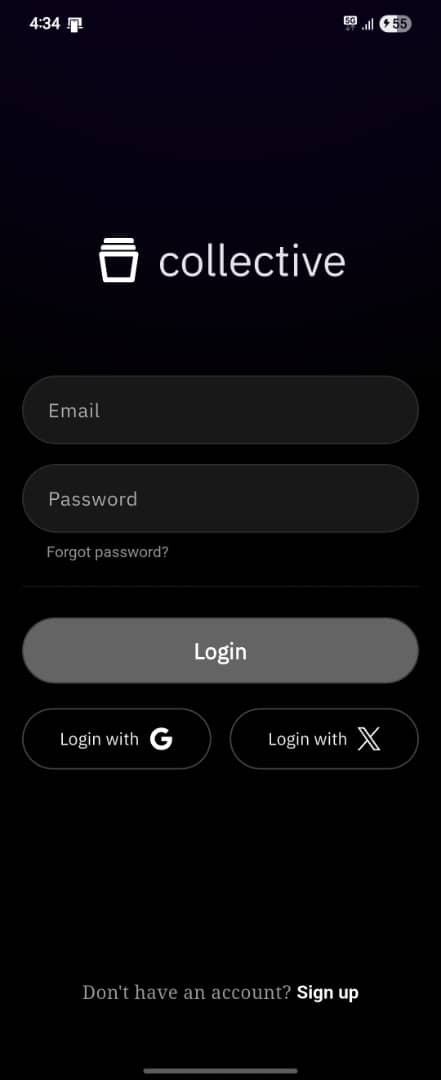
\includegraphics[width=0.35\textwidth]{files/imgs/prototype/auth_login.jpeg}
\caption{Login screen interface}
\label{fig:login-screen}
\end{figure}

\subsubsection{Registration Screen}

The registration screen expands the authentication interface to include additional fields for new user account creation. Users provide their first name, last name, email address, and password, with all fields featuring real-time validation to ensure data integrity and provide immediate feedback. The registration process includes email validation, password strength requirements, and clear visual indicators for required fields. Users can easily toggle between login and registration modes using the text link at the bottom of the screen.

\begin{figure}[H]
\centering
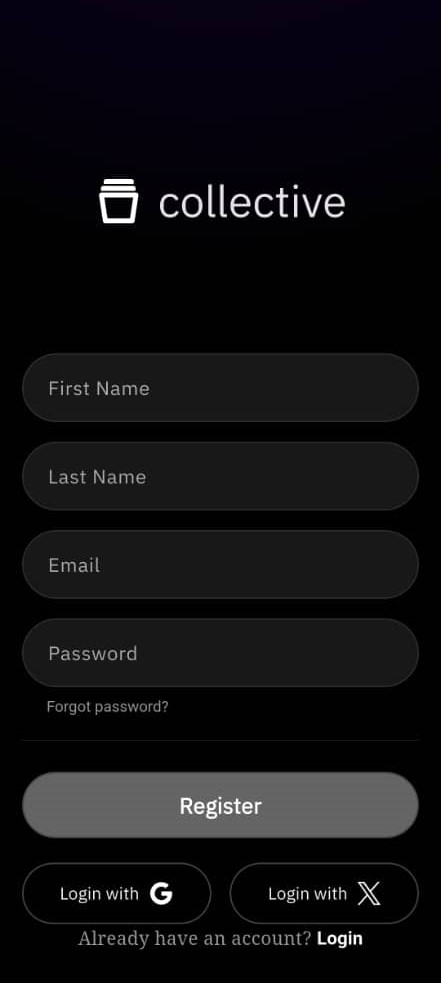
\includegraphics[width=0.35\textwidth]{files/imgs/prototype/auth_register.jpeg}
\caption{Registration screen with user details form}
\label{fig:registration-screen}
\end{figure}

\subsubsection{Google OAuth Integration}

The Google OAuth integration provides seamless authentication using existing Google accounts. The interface displays a dedicated button with the Google logo and clear labeling, allowing users to authenticate with a single tap without manual credential entry. The Google sign-in process leverages Firebase Authentication's OAuth provider, ensuring secure credential handling and automatic user profile creation upon successful authentication.

\subsubsection{Twitter/X OAuth Integration}

The Twitter/X OAuth integration offers an alternative social authentication method for users who prefer using their Twitter/X credentials. The interface includes a dedicated button with the Twitter/X logo, maintaining visual consistency with the Google OAuth option. The Twitter/X integration utilizes Firebase's OAuthProvider functionality with custom plugin modifications to ensure compatibility across different device configurations and handle edge cases in the authentication flow.

\begin{figure}[H]
\centering
\begin{minipage}{0.4\textwidth}
\centering
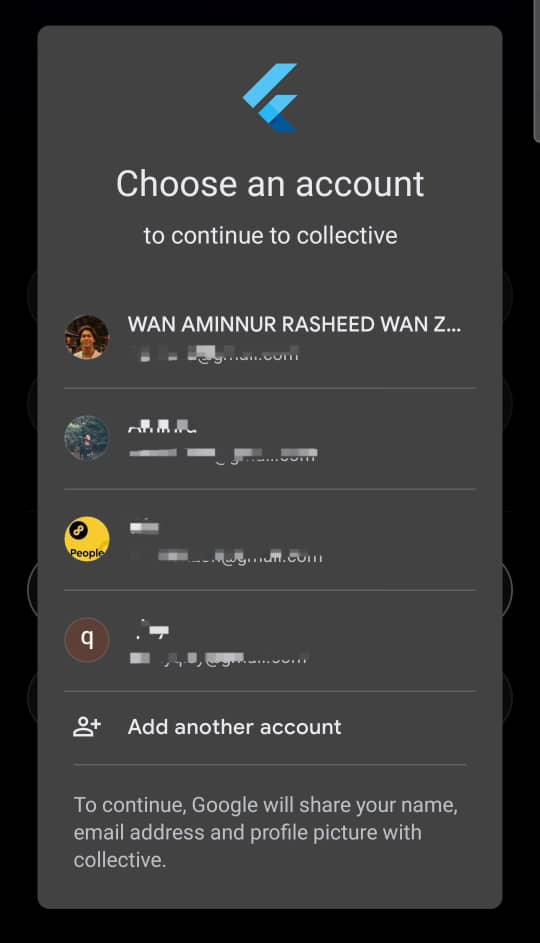
\includegraphics[width=0.8\textwidth]{files/imgs/prototype/google_oauth.jpeg}
\caption{Google OAuth authentication}
\label{fig:google-oauth}
\end{minipage}
\hfill
\begin{minipage}{0.4\textwidth}
\centering
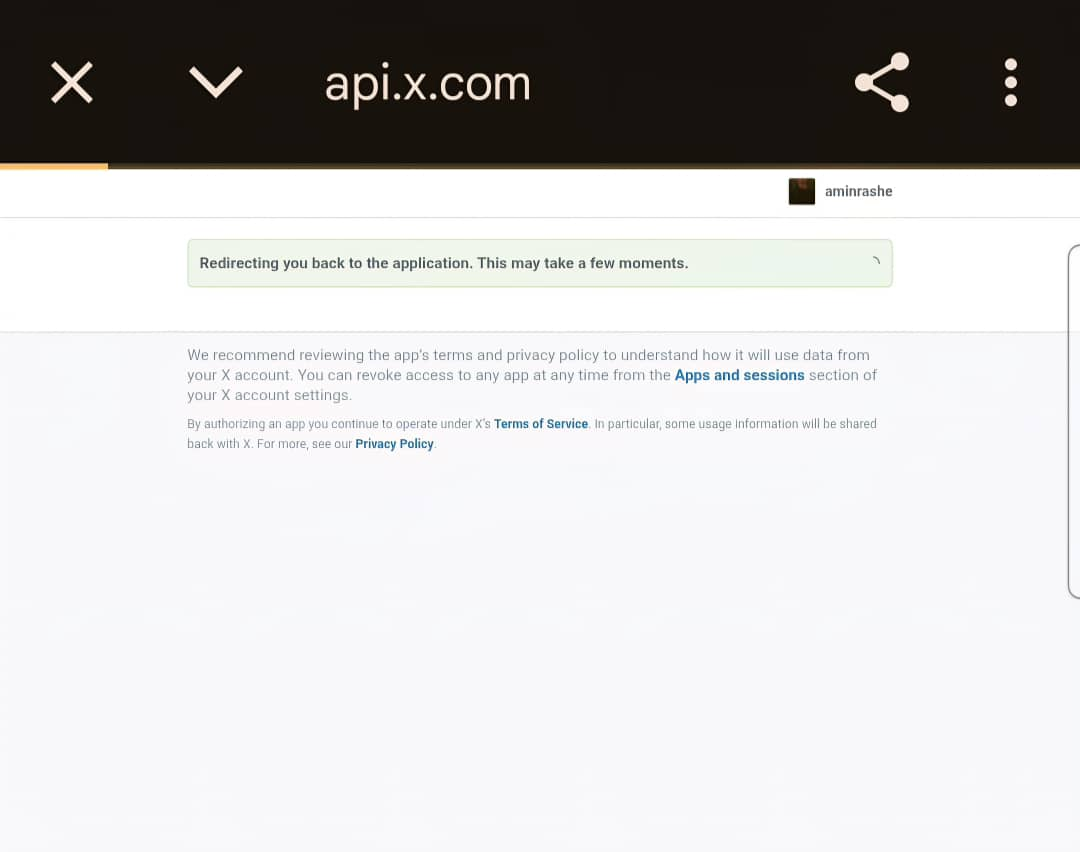
\includegraphics[width=0.8\textwidth]{files/imgs/prototype/x_oauth.jpeg}
\caption{Twitter/X OAuth authentication}
\label{fig:twitter-oauth}
\end{minipage}
\end{figure}

\subsection{Main Journal Interface}

\subsubsection{Journal Home Screen}

The journal home screen represents the core interface where users interact with their entries. The design prioritizes content over navigation, featuring a clean timeline view of journal entries organized by date. Each entry is displayed as a card with the date, content preview, mood indicator, and associated tags. The interface includes a search functionality and selection mode for batch operations like favoriting or deleting entries. The screen includes a toolbar with options for creating new entries, searching through existing content, and accessing analytics. Entries are grouped by date with sticky headers for easy navigation. The interface supports infinite scrolling and includes loading states with shimmer effects for smooth user experience.

\begin{figure}[H]
\centering
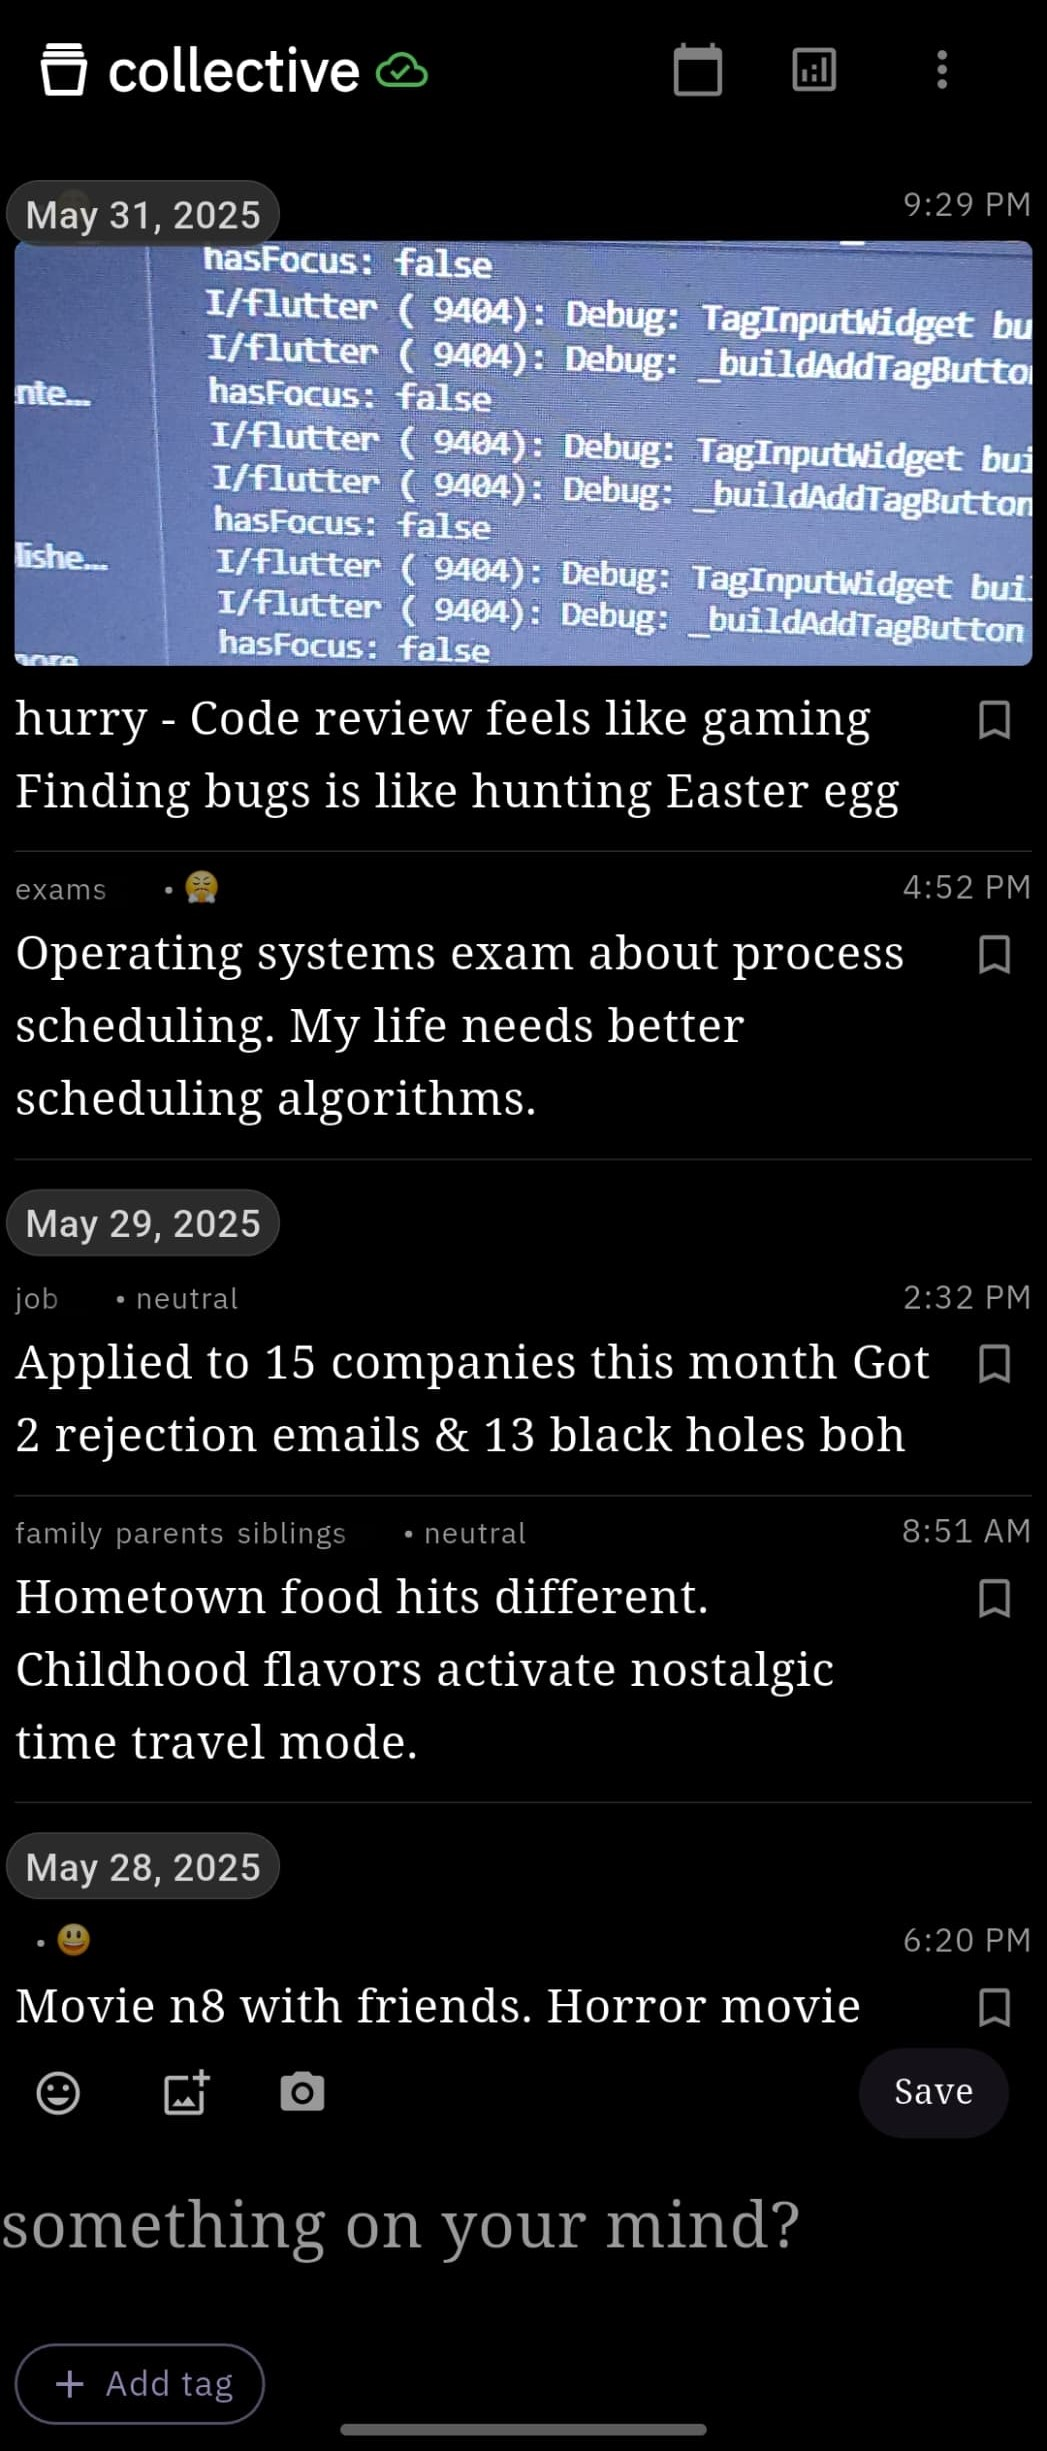
\includegraphics[width=0.4\textwidth]{files/imgs/prototype/journal_screen.jpeg}
\caption{Journal home screen showing entry timeline}
\label{fig:journal-screen}
\end{figure}

\subsubsection{Journal Input Interface}

The journal input interface emphasizes distraction-free writing with a minimalist text editor that expands as users type. The interface includes subtle features like mood selection through emoji picker, tag input with AI-powered suggestions, and multimedia attachment capabilities including camera integration for photos and GIF creation. The interface includes automatic saving to prevent data loss and provides visual feedback for all user actions.

\begin{figure}[H]
\centering
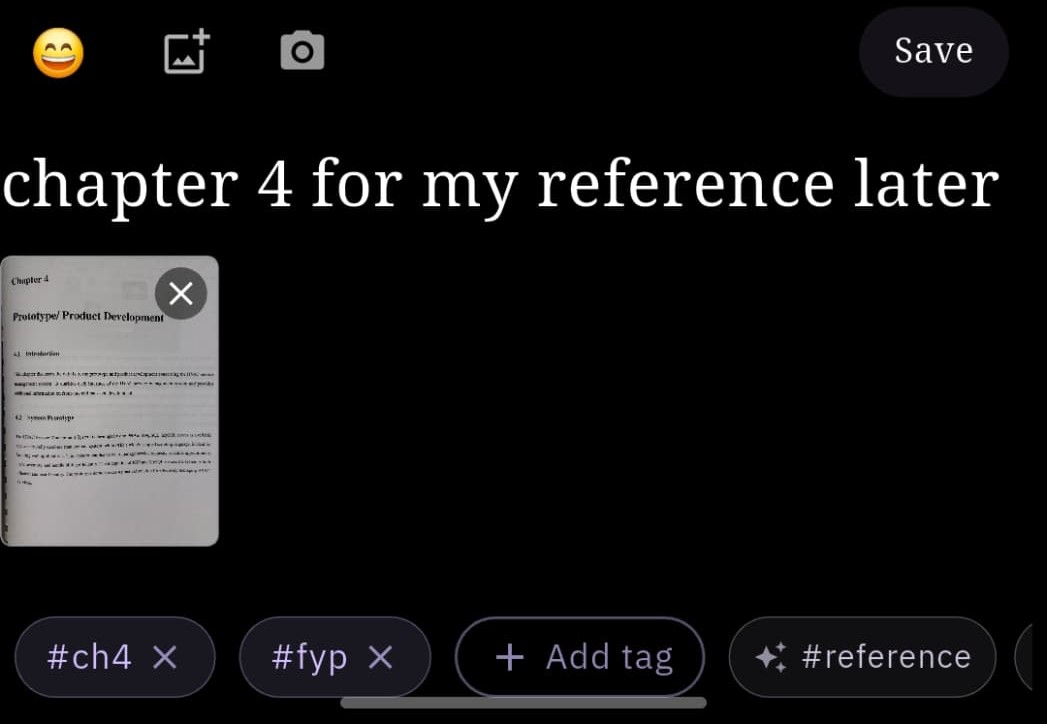
\includegraphics[width=0.4\textwidth]{files/imgs/prototype/journal_input_basic.jpeg}
\caption{Basic journal input interface for writing entries}
\label{fig:journal-input-basic}
\end{figure}

\paragraph{Emoji Selection Interface}

The emoji selection feature provides an expandable emoji bar for mood selection. Users can tap to reveal a collection of mood-representing emojis that help categorize their emotional state while writing. The emoji bar integrates seamlessly with the writing interface without disrupting the flow of composition.

\begin{figure}[H]
\centering
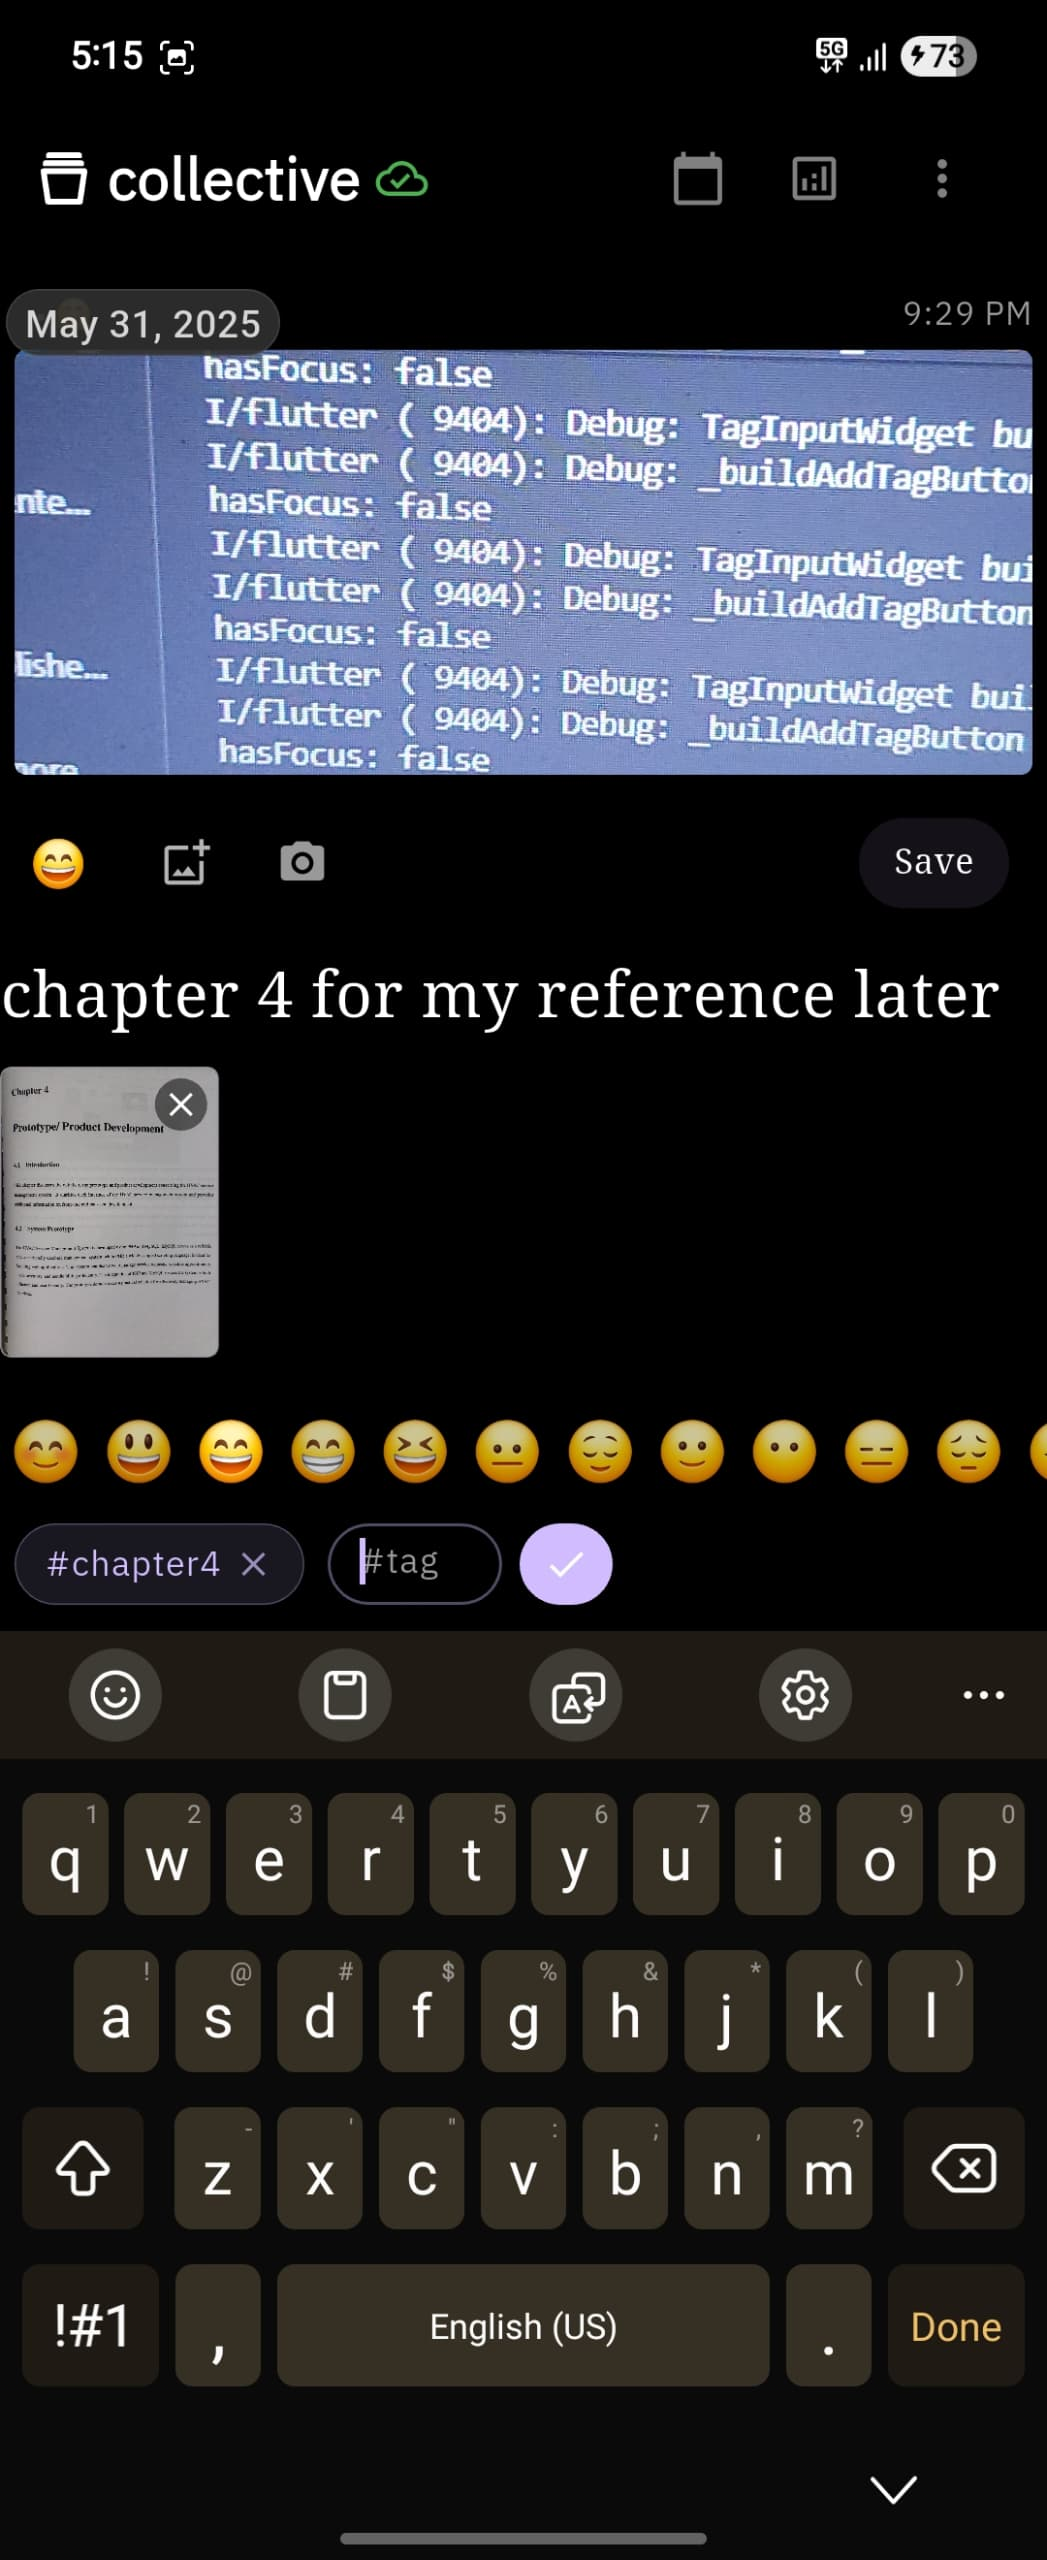
\includegraphics[width=0.4\textwidth]{files/imgs/prototype/emoji_selection.jpeg}
\caption{Emoji selection interface for mood indication}
\label{fig:emoji-selection}
\end{figure}

\paragraph{Photo Attachment Interface}

The photo attachment functionality allows users to add visual content to their journal entries. The interface provides options to select existing photos from the device gallery or capture new images using the camera. Photos are automatically compressed and optimized for storage while maintaining visual quality.

\begin{figure}[H]
\centering
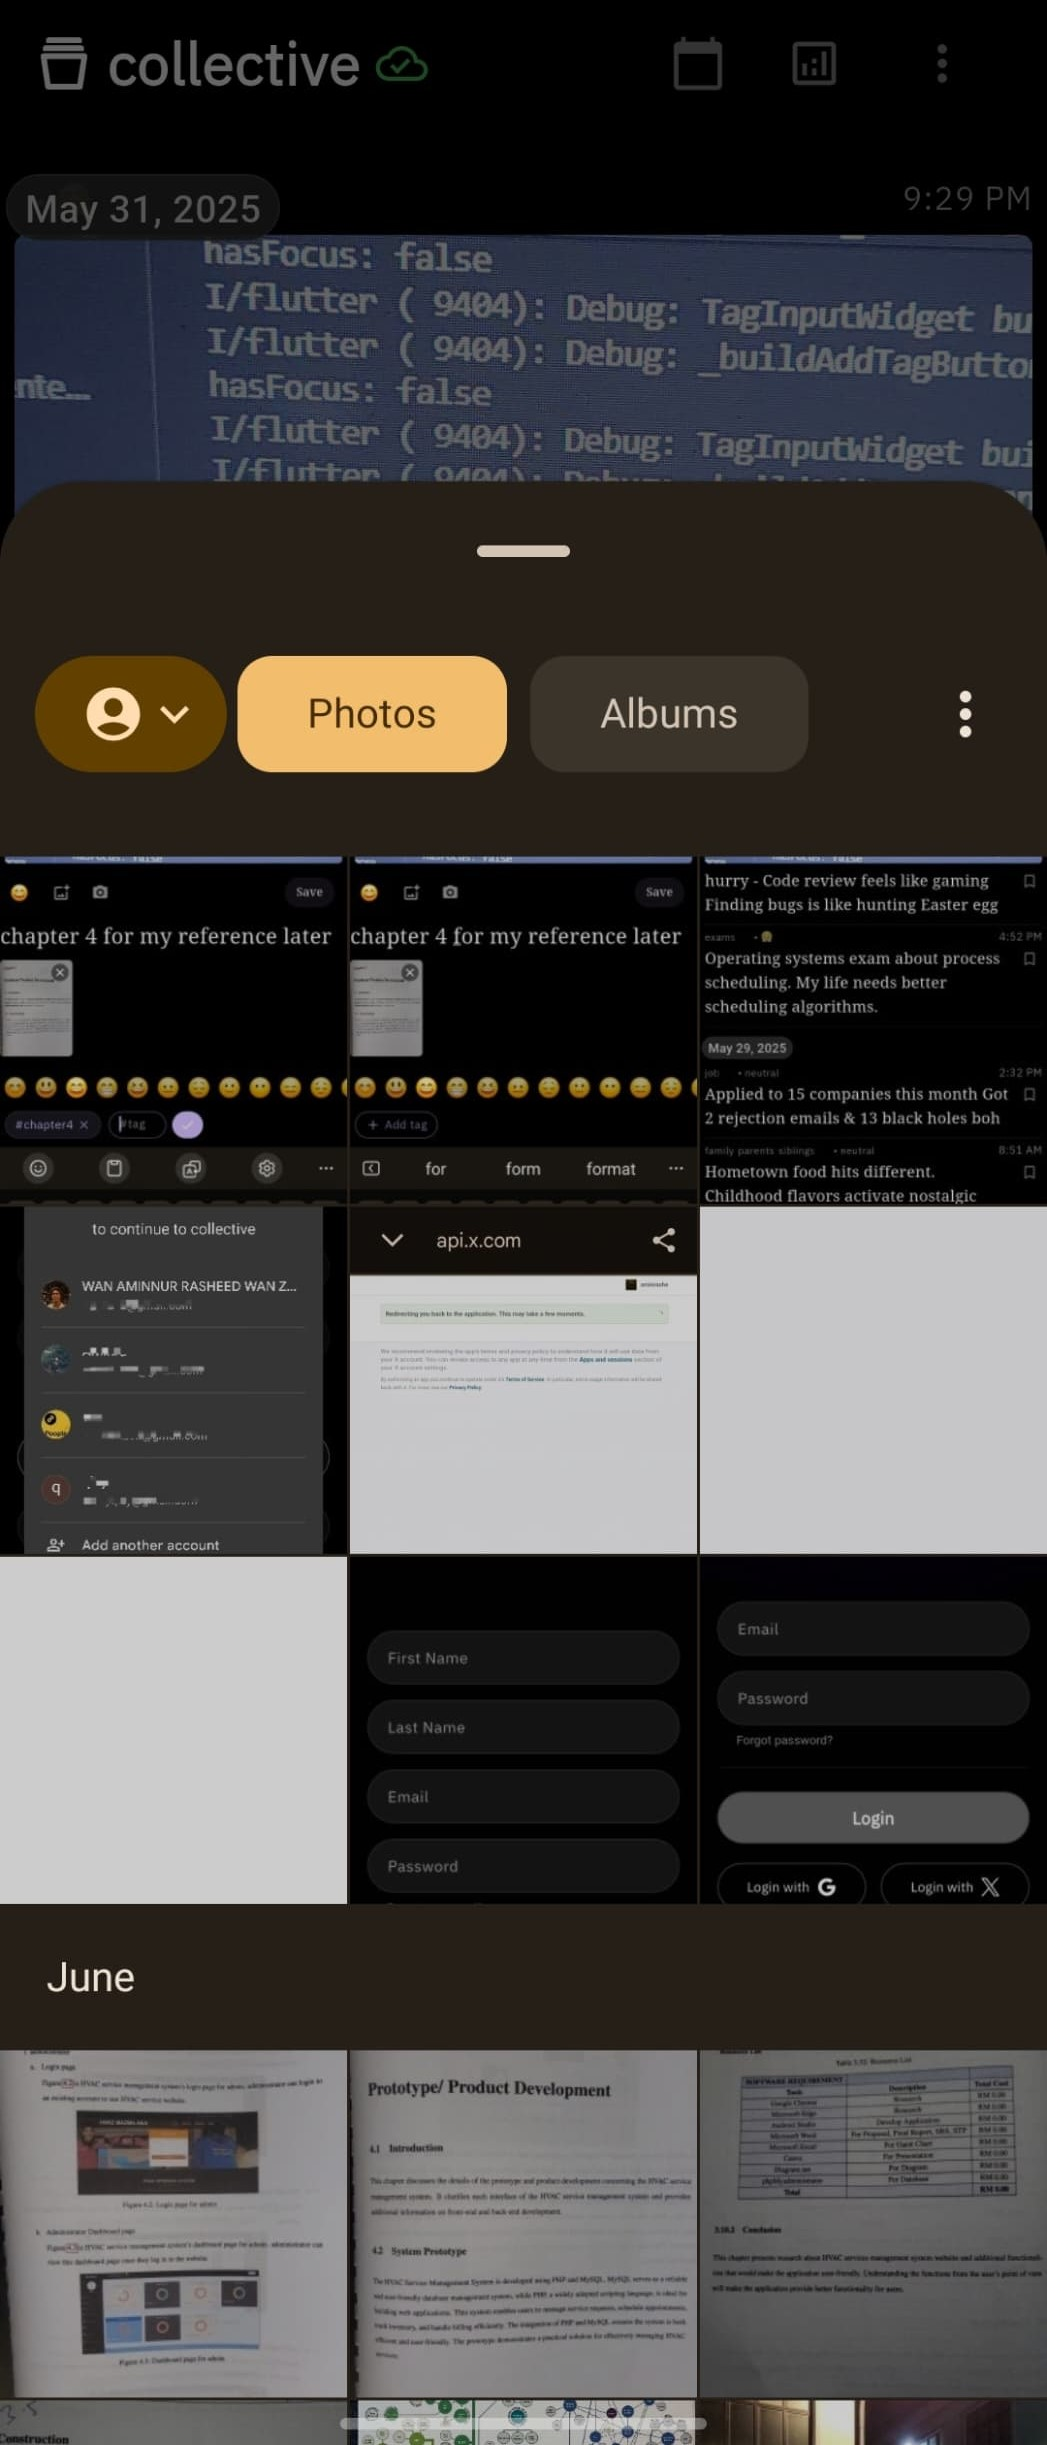
\includegraphics[width=0.4\textwidth]{files/imgs/prototype/photo_attachment.jpeg}
\caption{Photo attachment interface for adding images}
\label{fig:photo-attachment}
\end{figure}

\paragraph{Camera Integration}

The camera integration feature enables users to capture moments directly within the journal interface. The camera preview appears seamlessly within the app, allowing for immediate photo capture without leaving the writing context. The interface maintains focus on journaling while providing powerful multimedia capabilities.

\begin{figure}[H]
\centering
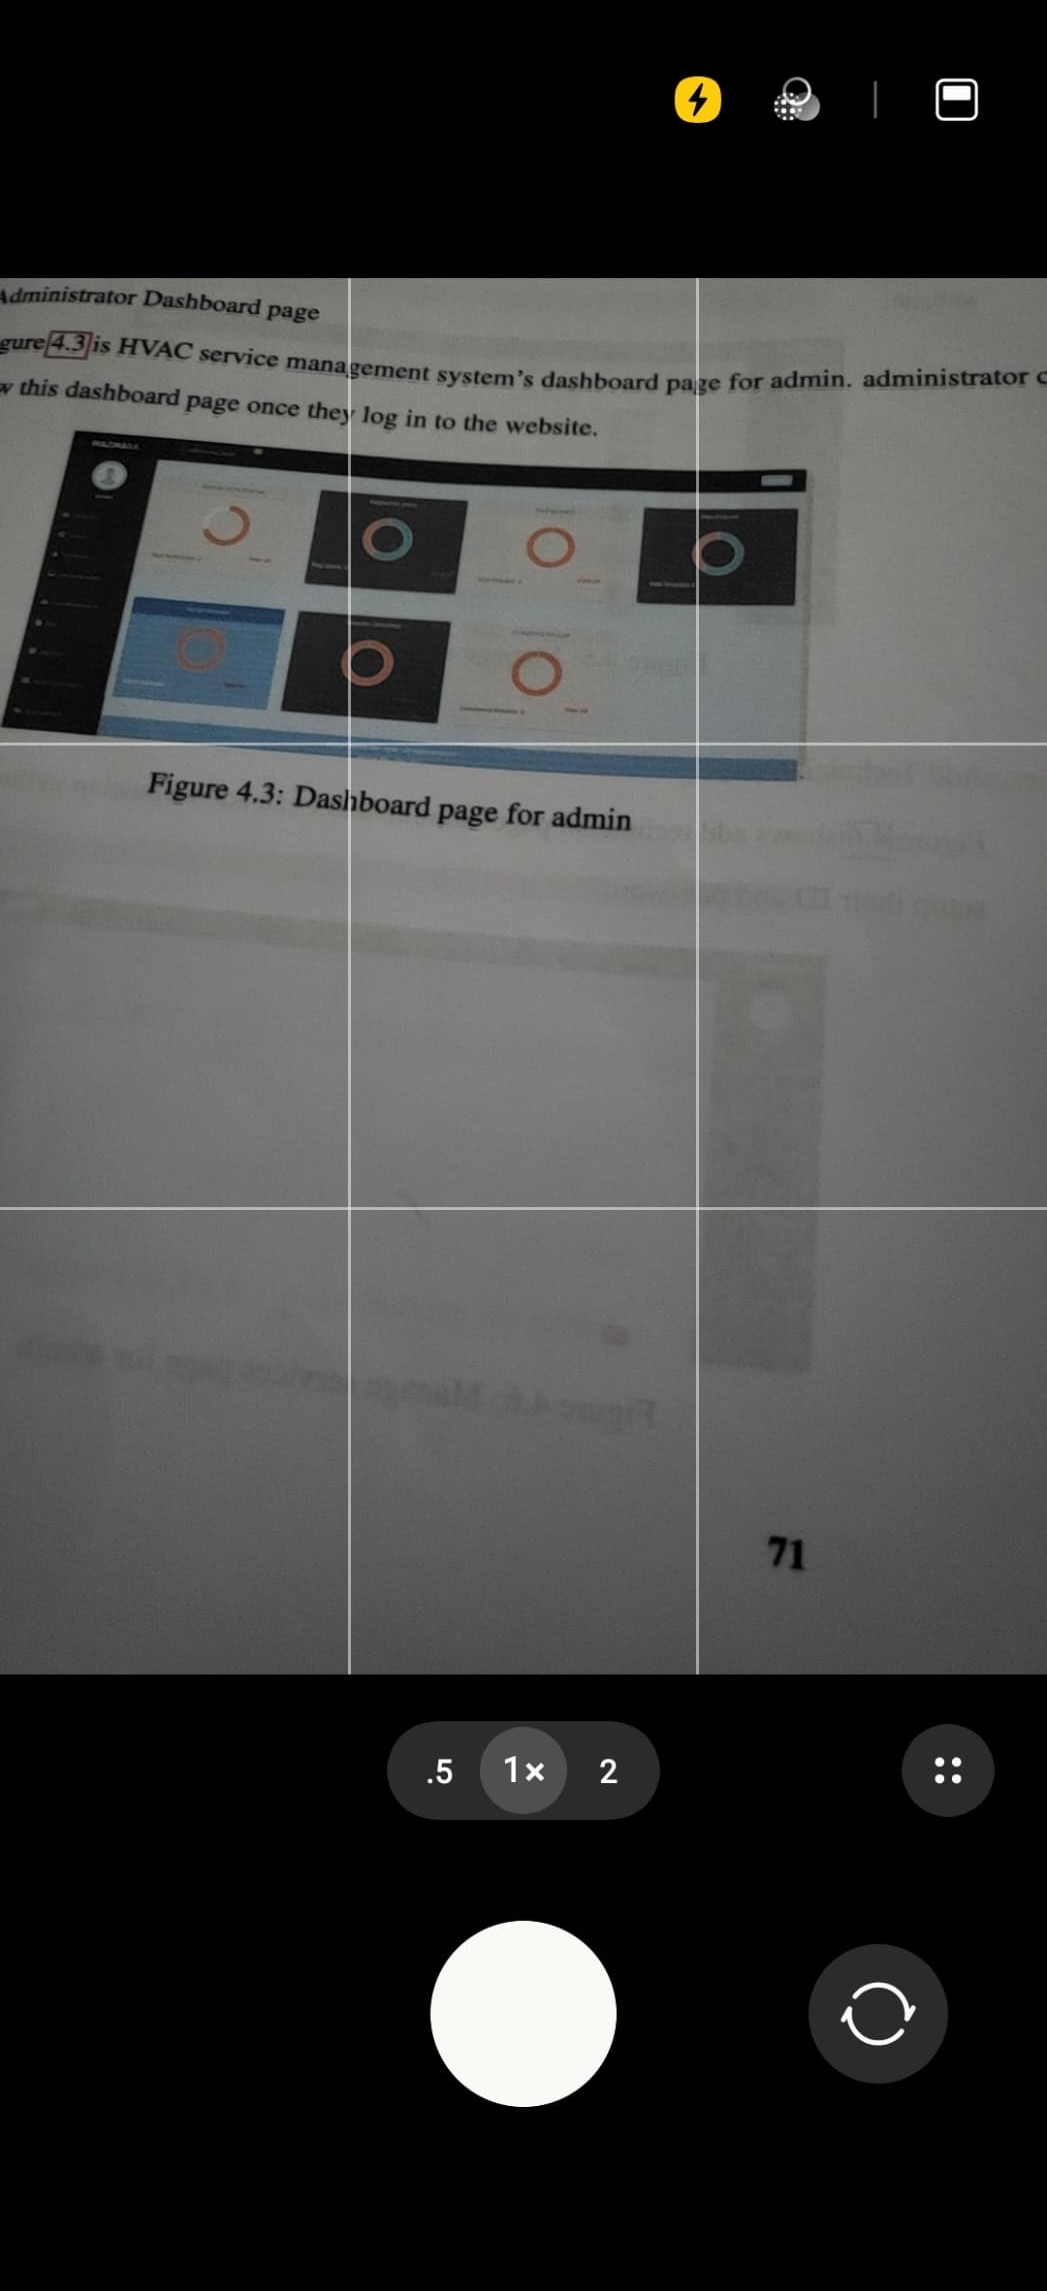
\includegraphics[width=0.4\textwidth]{files/imgs/prototype/camera_interface.jpeg}
\caption{Integrated camera interface for direct photo capture}
\label{fig:camera-interface}
\end{figure}

\paragraph{GIF Recording Functionality}

The GIF recording feature allows users to create short animated sequences to capture dynamic moments. Users can record brief video clips that are automatically converted to GIF format using FFmpeg processing. This feature adds a unique multimedia dimension to traditional journaling while maintaining storage efficiency.

\begin{figure}[H]
\centering
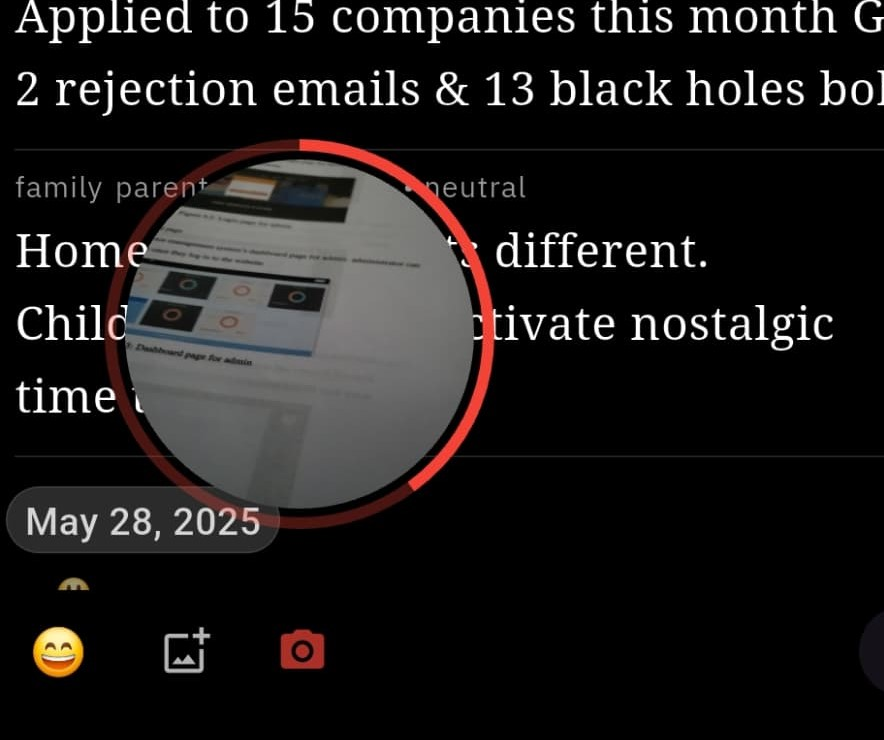
\includegraphics[width=0.4\textwidth]{files/imgs/prototype/gif_recording.jpeg}
\caption{GIF recording interface for creating animated content}
\label{fig:gif-recording}
\end{figure}

\paragraph{AI-Powered Tag Suggestions}

The tag suggestion system utilizes AI analysis to recommend relevant tags based on the entry content. As users type, the system analyzes the text in real-time and suggests contextually appropriate tags that help organize and categorize journal entries. The suggestions appear as subtle prompts that users can accept or ignore according to their preferences.

\begin{figure}[H]
\centering
\begin{minipage}{0.45\textwidth}
\centering

\includegraphics[width=0.9\textwidth]{files/imgs/prototype/tag_input.jpeg}
\caption{Tag input interface}
\label{fig:tag-input}
\end{minipage}
\hfill
%\begin{minipage}{0.45\textwidth}
%\centering
%\includegraphics[width=0.9\textwidth]{path/to/tag_suggestions.png}
%\caption{AI-powered tag suggestions}
%\label{fig:tag-suggestions}
%\end{minipage}
\end{figure}

\subsection{Entry Management}

\subsubsection{Entry Insight Screen}

The entry insight screen provides detailed analysis of individual journal entries using AI-powered insights from DeepSeek API. The screen displays the full entry content along with AI-generated insights that help users understand patterns in their writing and emotional state. Related entries are suggested based on content similarity and themes. The insights are presented in markdown format with smooth loading animations and caching for offline access. The screen includes navigation to related entries and maintains a history of viewed insights for quick reference.

\subsubsection{Edit Entry Screen}

The edit entry screen allows users to modify existing journal entries while maintaining the original creation timestamp. The interface provides the same rich editing capabilities as the input widget, including mood modification, tag editing, and image management. Changes are tracked and saved automatically with visual feedback. The screen includes options to add or remove images, modify mood settings, and update tags. All changes are validated and synchronized with both local and cloud storage.

\begin{figure}[H]
\centering
\begin{minipage}{0.45\textwidth}
\centering
\includegraphics[width=0.85\textwidth]{files/imgs/prototype/entry_insight_screen.jpeg}
\caption{Entry insight screen with AI analysis}
\label{fig:entry-insight-screen}
\end{minipage}
\hfill
\begin{minipage}{0.45\textwidth}
\centering
\includegraphics[width=0.85\textwidth]{files/imgs/prototype/edit_entry_screen.jpeg}
\caption{Edit entry screen for modifying entries}
\label{fig:edit-entry-screen}
\end{minipage}
\end{figure}

\subsection{Analytics and Insights}

\subsubsection{Analytics Dashboard}

The analytics screen presents comprehensive insights into journaling patterns and trends using visual representations of data. The interface includes calendar views showing journaling frequency, topic clustering analysis, and mood tracking over time. The analytics are generated using AI analysis of journal content while maintaining user privacy. Key features include topic clustering cards that group related entries, calendar heat maps showing writing frequency, and insights panels with AI-generated observations about writing patterns. The analytics cache intelligently to reduce processing time and API usage.

\begin{figure}[H]
\centering
\includegraphics[width=0.4\textwidth]{files/imgs/prototype/analytics_screen.jpeg}
\caption{Analytics dashboard showing journaling patterns}
\label{fig:analytics-screen}
\end{figure}

\subsubsection{Topic Clustering Visualization}

The topic clustering feature automatically groups journal entries by themes and subjects using AI analysis. Each cluster is presented as a card showing the main topic, number of entries, and key themes. Users can explore clusters to find related content across different time periods.

\begin{figure}[H]
\centering
\includegraphics[width=0.4\textwidth]{files/imgs/prototype/topic_clustering.jpeg}
\caption{Topic clustering visualization}
\label{fig:topic-clustering}
\end{figure}

\subsection{Favorites and Collections}

\subsubsection{Favorites Screen}

The favorites screen displays a curated collection of entries that users have marked as favorites. The interface follows the same design patterns as the main journal screen but filters to show only favorited content. Entries maintain their original date grouping and include all standard interaction options. Users can easily unfavorite entries and access all entry details and insights from this screen. The interface provides quick access to frequently referenced content.

\begin{figure}[H]
\centering
\includegraphics[width=0.4\textwidth]{files/imgs/prototype/favorites_screen.jpeg}
\caption{Favorites screen showing curated entries}
\label{fig:favorites-screen}
\end{figure}

\section{Technical Implementation Details}

\subsection{Frontend Architecture}

The Flutter frontend implements a controller-based architecture using JournalController as the central state management system. The UI components follow Material Design 3 principles while incorporating custom styling that reflects the application's focus on simplicity and elegance. Animation controllers are properly managed to prevent memory leaks and ensure smooth transitions.

\subsection{Backend Integration}

Firebase integration provides seamless authentication, cloud storage for images and data, and real-time synchronization capabilities. The system implements intelligent caching strategies to minimize data usage while ensuring offline functionality remains robust. Local storage uses Sembast database for structured data and file system for images.

\subsection{AI Service Integration}

DeepSeek API integration follows a streaming response pattern, providing real-time insights as analysis occurs. The system implements comprehensive fallback mechanisms for API failures, ensuring the core journaling functionality remains unaffected by external service availability. Insights are cached both in memory and persistent storage to improve performance.

\subsection{Multimedia Handling}

The application includes sophisticated camera integration with support for both photo capture and GIF creation using FFmpeg. Images are processed and compressed for optimal storage while maintaining quality. The system supports both local and cloud storage with automatic synchronization.

\section{User Experience Design}

The interface design prioritizes simplicity and focus, removing unnecessary navigation elements and feature complexity that typically overwhelms users in digital journaling applications. The use of consistent spacing, typography, and color schemes creates a cohesive experience that feels familiar and comfortable.

System theme integration ensures the application feels native to each user's device preferences, while careful attention to loading states and animations maintains engagement during processing operations. The offline-first approach ensures users never lose their writing due to connectivity issues.

\section{Quality Assurance and Testing}

The prototype undergoes continuous testing through multiple approaches including unit testing for core functionality, integration testing for service interactions, and user acceptance testing with target demographics. Performance testing ensures smooth operation across various mobile devices and operating system versions.

Specific attention is paid to edge cases such as network interruptions, device storage limitations, and API service outages to ensure robust operation in real-world conditions.

\section{Summary}

The Collective journaling application prototype successfully demonstrates the integration of traditional journaling intimacy with modern digital capabilities. Through careful interface design and intelligent feature implementation, the system addresses the identified problems of digital journaling complexity while maintaining the personal, reflective nature that makes journaling valuable. The technical architecture ensures reliability, privacy, and accessibility across platforms while providing sophisticated AI-powered insights that enhance rather than replace the human journaling experience.
\chapter{Testing and Result}\label{ch:testing}

\section{Introduction}\label{sec:testingIntroduction}

This chapter provides an overview of the testing scenarios associated with the \textbf{Collective} mobile journaling application. The importance of testing in the software development life cycle is paramount, as it ensures that the system operates reliably and meets user requirements. The primary goal of testing is to identify and resolve technical issues and bugs, ensuring the system functions correctly and aligns with the specified requirements outlined in Chapter~\ref{ch:methodology}.

Testing the Collective mobile journaling application involves evaluating the system's various functionalities including journal entry creation, user authentication, data storage and synchronization, AI-powered insights, and offline capabilities. Due to the complexity of the mobile application and the numerous possible input and output combinations across different Android devices, it is impractical to test every possible scenario. However, thorough testing aims to cover as many scenarios as possible to ensure robustness and reliability.

The chapter emphasizes four critical testing methodologies: \textbf{Integration Testing} to verify component interaction, \textbf{System Testing} to validate overall functionality, \textbf{User Acceptance Testing} with test cases specified in individual tables, and \textbf{Usability Testing} conducted through structured feedback gathering with respondents as testers. By adhering to these testing standards, the chapter aims to demonstrate how the Collective mobile journaling application meets quality standards and fulfills user requirements.

\section{Test Objective}\label{sec:testObjective}

The test plan focuses on identifying and documenting as many bugs as possible to enhance the system's reliability. The \textbf{Collective} mobile journaling application underwent extensive testing through four testing phases: Integration Testing to verify component interactions, System Testing to validate complete functionality, User Acceptance Testing with test cases documented in individual tables, and Usability Testing conducted through structured feedback gathering with respondents as testers.

The application testing focused on crucial operations such as journal entry creation, editing, deletion, user authentication, data synchronization, and AI-powered insights generation. The user interface has been carefully crafted to ensure ease of use, facilitating smooth navigation throughout the journaling experience. Throughout the development process, emphasis has been placed on performance and usability to ensure a seamless journaling experience.
\chapter{Conclusions and Suggestions}\label{ch:conclusions}

\section{Introduction}\label{sec:conclusionsIntroduction}

This chapter will describe the entire process of developing and managing the Collective mobile journaling application. It will discuss the key components of the project and share valuable lessons learned throughout the development journey. This information will serve as a useful reference for future mobile application development projects. Additionally, this chapter will include suggestions for future improvements to improve the application's functionality and user experience.

The Collective mobile journaling application represents a comprehensive solution that connects traditional and digital journaling approaches, incorporating modern technologies such as Flutter framework, Firebase cloud services, and AI-based insights through DeepSeek API integration. This final chapter consolidates the project achievements, evaluates the outcomes against initial objectives, and provides recommendations for continued development.

\section{Accomplishment}\label{sec:accomplishment}

The Collective mobile journaling application project has successfully achieved its main goals and reached its final development stage. The development team carried out extensive research, user studies, iterative design processes, and comprehensive testing, overcoming various technical and design challenges to ensure the project's success.

\subsection{Core Objectives Achievement}

The system has met all its fundamental objectives and implemented all specified features as outlined in Chapter~\ref{ch:methodology}. The application addresses the key problems identified in traditional digital journaling applications, including complexity barriers, poor offline functionality, and lack of meaningful insights generation.

\textbf{Primary Achievements:}

\textbf{i. Simplified User Experience:} The application achieved a 100\% positive feedback rate for user interface design and 90\% positive feedback for navigation ease, as demonstrated in the usability testing results. The minimalist design approach successfully eliminates complexity barriers that cause abandonment in traditional journaling applications.

\textbf{ii. Offline-First Design:} Implemented comprehensive offline functionality using Sembast local database with automatic Firebase cloud synchronization. The system maintains 80\% user satisfaction for offline capabilities, enabling users to journal without internet connectivity while ensuring data integrity across devices.

\textbf{iii. AI-Based Insights Integration:} Integrated DeepSeek API to provide contextual analysis and pattern recognition, achieving 90\% positive user feedback for AI insights functionality. The system generates meaningful emotional patterns, content analysis, and personalized recommendations without compromising user privacy.

\textbf{iv. Multi-Platform Compatibility:} Developed using Flutter framework to ensure consistent performance across different Android devices and API levels (21-34), providing a native mobile experience with optimized performance and battery efficiency.

\textbf{v. Comprehensive Feature Set:} Implemented all planned features including journal entry creation and editing, mood tracking, image attachments, search functionality, analytics dashboard, bookmark management, theme switching, and social authentication options.

\subsection{Technical Accomplishments}

The project has provided valuable experience in managing complex mobile application development, and the development team has gained expertise in modern software engineering practices, cross-platform mobile development, cloud integration, and AI service implementation.

\textbf{Technical Milestones:}

\textbf{i. Architecture Design:} Implemented a scalable, maintainable architecture following Flutter best practices with proper separation of concerns between UI components, business logic services, and data management layers.

\textbf{ii. Database Management:} Designed and implemented dual database strategy with local Sembast storage for offline capabilities and Firebase Firestore for cloud synchronization, ensuring data consistency and integrity.

\textbf{iii. API Integration:} Integrated multiple external services including Firebase Authentication, Firebase Storage, DeepSeek AI API, and social OAuth providers (Google and Twitter/X) with proper error handling and fallback mechanisms.

\textbf{iv. Performance Optimization:} Achieved satisfactory performance metrics with 90\% positive user feedback for application speed and responsiveness, implementing efficient data caching, image compression, and background synchronization.

\subsection{User Validation Success}

The comprehensive usability testing with UniKL student respondents validated the application's effectiveness in meeting its design objectives. With an overall average rating of 4.35/5.0 and 91.6\% positive feedback across all evaluation criteria, the application demonstrates achievement of user requirements and expectations.

The testing results particularly validate the core design philosophy of providing a distraction-free journaling experience, achieving 90\% positive feedback for this primary objective. The application connects traditional and digital journaling approaches while maintaining the personal, focused experience that users value in traditional journaling.

\section{Recommendation}\label{sec:recommendation}

Although the Collective mobile journaling application has achieved its goals and served its intended purpose, there are still areas for improvement identified through user feedback and development experience. Continuous improvement is essential for the application's long-term success and user adoption. To make the application more effective and competitive, it is recommended to focus on improving the following aspects:

\subsection{Performance and Technical Enhancements}

\textbf{i. Performance Optimization:} Based on user feedback indicating room for improvement in loading speed and responsiveness, implement additional caching strategies, optimize database queries, and improve image loading performance. Consider implementing progressive loading for large journal collections and optimize AI processing response times.

\textbf{ii. Improved Offline Synchronization:} Address the synchronization challenges identified in user testing (80\% satisfaction rate) by implementing more reliable conflict resolution mechanisms, better connectivity detection, and improved sync status indicators to keep users informed of synchronization progress.

\textbf{iii. Additional AI Capabilities:} Expand the AI analysis features to include more sophisticated pattern recognition, mood trend predictions, and personalized writing prompts. Consider implementing local AI processing for basic insights to reduce dependency on external APIs and improve response times.

\subsection{Feature Expansion Recommendations}

\textbf{i. Multi-Platform Support:} Extend the application to iOS platform to reach a broader user base and ensure feature parity across both major mobile platforms. Implement web application support for users who prefer journaling on desktop or tablet devices.

\textbf{ii. Collaborative Features:} Introduce optional sharing capabilities for users who wish to share selected journal entries with trusted contacts, while maintaining privacy controls and user consent mechanisms.

\textbf{iii. Additional Analytics and Insights:} Implement more comprehensive analytics including writing pattern analysis, goal tracking with progress visualization, and personalized recommendations for journaling habits improvement.

\subsection{User Experience Improvements}

\textbf{i. Accessibility Enhancements:} Implement comprehensive accessibility features including voice-to-text input, screen reader compatibility, and adjustable font sizes to ensure the application is usable by users with diverse needs and abilities.

\textbf{ii. Customization Options:} Provide additional customization options including custom themes, personalized layouts, configurable notification settings, and flexible export formats to accommodate diverse user preferences.

\textbf{iii. Data Export and Backup:} Implement comprehensive data export functionality allowing users to backup their journal entries in multiple formats (PDF, text, HTML) and ensure users maintain control over their personal data.

\subsection{Security and Privacy Enhancements}

\textbf{i. Enhanced Encryption:} Implement end-to-end encryption for journal entries to ensure maximum privacy protection, particularly for users storing sensitive personal information.

\textbf{ii. Biometric Authentication:} Add biometric authentication options (fingerprint, face recognition) to provide additional security layers while maintaining ease of access for legitimate users.

\textbf{iii. Privacy Controls:} Provide granular privacy controls allowing users to specify which data can be processed by AI services and which entries should remain completely private and local-only.

\section{Conclusion}\label{sec:conclusion}

In summary, the Collective mobile journaling application project has achieved its purpose and goals by completing a comprehensive digital journaling solution within the allotted time frame and gaining approval from the supervisor. The main objectives of connecting traditional and digital journaling approaches while providing a simplified, distraction-free user experience were fulfilled, ensuring that the application met the necessary criteria and delivered the anticipated results.

The project demonstrated the effectiveness of combining modern mobile development technologies with thoughtful user experience design. The Flutter framework proved excellent for multi-platform development, Firebase provided reliable cloud infrastructure, and the DeepSeek AI integration added meaningful value without compromising the core journaling experience. The offline-first design ensures users can maintain their journaling habits regardless of connectivity, while the AI-based insights provide valuable personal growth opportunities.

Despite facing various technical challenges including API integration complexities, offline synchronization implementation, and performance optimization requirements, the project offered valuable lessons and opportunities for professional growth. The development experience provided expertise in mobile application development, cloud service integration, AI API implementation, user experience design, and comprehensive software testing methodologies.

The comprehensive usability testing validated the application's success with 91.6\% positive feedback across all evaluation criteria and an overall average rating of 4.35/5.0. The application successfully achieved its core objective of providing a distraction-free journaling experience, receiving 90\% positive feedback for this primary goal. User feedback particularly praised the clean, minimalist interface design, intuitive navigation, and effective AI insights functionality.

The project contributes valuable insights to the field of digital journaling applications, demonstrating that it is possible to create sophisticated mobile applications that maintain the personal and focused qualities of traditional journaling while utilizing modern technologies for improved functionality. The research and development process revealed important considerations for mobile application design, particularly the balance between feature richness and simplicity that users value in personal productivity applications.

It is expected that the Collective mobile journaling application will provide benefits to its users, supporting their personal growth, emotional well-being, and reflective practices. The application serves as a foundation for future development in the digital journaling space and demonstrates the potential for AI-enhanced personal productivity tools that respect user privacy while providing meaningful insights.

The completion of this project represents not only a functional mobile application but also a comprehensive research and development exercise that advances understanding of user needs in digital journaling, effective mobile application architecture design, and the integration of AI technologies in personal productivity applications. The lessons learned and methodologies developed throughout this project will serve as valuable references for future mobile application development endeavors in the personal productivity and digital wellness domains.

% You can add a new chapter by copying the above command and changing its name to the new chapter name. This command will include a new chapter file in your thesis. After this, create a new Tex file with the same name you have given above and save this file in the "files" folder of your thesis directory. %
	
	
% -----------------------------------------------------------------------

\addcontentsline{toc}{chapter}{\bibname}
%\bibliographystyle{IEEEtran}
\bibliographystyle{apalike}

%One bibliography
\bibliography{bib/thesis}

\appendix
\numberwithin{figure}{chapter} 

% ---------------------------------------------------------------------
% annexures 
\makeappendixseperator
\singlespacing
\chapter{Gantt Chart}\label{appendix-a}


\section{Construction of Variables} 


\chapter{Questionnaire Sample}\label{appendix-b}

The Questionnaire for this research.

\end{document} 

 